\documentclass[12pt,a4paper]{DOLthesis}  
%\documentclass[12pt,a4paper,twoside]{DOLthesis}  %twoside document
%load any additional packages
\usepackage[british]{babel}
% To ammend errors and warnings
\RequirePackage{etex}
\usepackage{csquotes}
%%
\usepackage{enumitem}
\usepackage{tikz}
\usepackage{lscape}
\usepackage{longtable}
\usepackage{multirow,bigdelim,dcolumn,booktabs}
\usepackage{graphicx}
\usepackage{floatrow}
\usepackage{subfig}
\usepackage{pgfplots}
\pgfplotsset{width=0.8\linewidth,compat=1.9}
\usepackage{chemfig} 			%for chemical structures
\setatomsep{2.5em}                %bond length. 3em is the standard

\usepackage{tkz-fct}
\usetikzlibrary{external}		%to speed up figures
%\tikzexternalize[prefix=tikz/]%,shell escape=-enable-write1 --shell-escape,prefix=tikz/, mode=graphics if exists, export=false, optimize=false
% \tikzset{
% 	png export/.style={
% 		external/system call/.add=
% 		{}
% 		{; convert -density 300 -transparent white "\image.pdf" -quality 100 "\image.png";},
% 		%
% 		/pgf/images/external info,
% 		/pgf/images/include external/.code={%
% 			\includegraphics
% 			[width=\pgfexternalwidth,height=\pgfexternalheight]
% 			{##1.png}%
% 		}
% 	}
% }

\usepackage[style=nature,%chem-acs,%phys,nature
sorting=none,sortcites=true, giveninits=true,hyperref, doi=false,eprint=false,url=false,isbn=false]{biblatex}	
\addbibresource{refs_new.bib}
\addbibresource{mendeley_refs.bib}
\AtEveryBibitem{\clearfield{note}}
\renewbibmacro{in:}{}

\usepackage{booktabs}
\usepackage[symbol]{footmisc}
\renewcommand{\thefootnote}{\fnsymbol{footnote}}
\usepackage[left=2cm,top=3cm,right=2cm,bottom=3cm,bindingoffset=1cm]{geometry}
\usepackage{amssymb}
\usepackage{amsmath}
\usepackage[page,toc,titletoc,title]{appendix}
\usepackage[justification=centering]{caption}
\captionsetup{font={stretch=1.5}}
\usepackage{textcomp}
\usepackage{pdfpages} 
\usepackage{hyperref}
\hypersetup{colorlinks,citecolor=black,filecolor=black,linkcolor=black,urlcolor=black}
\usepackage{datetime}
\newdateformat{monthyeardate}{%
  \monthname[\THEMONTH] \THEYEAR}
  
\usepackage{sectsty}
\chapterfont{\centering}              %this centers the chapters title

\usepackage{blindtext}

%these packages are for captions on top of tables
\usepackage{float}			
\floatstyle{plaintop}
\restylefloat{table}

\usepackage[doublespacing]{setspace}        %double space

\usepackage{longtable}
\usepackage[acronym]{glossaries}
\usepackage{glossary-mcols}
\makenoidxglossaries
\newacronym{}{}{}

% cited
\newacronym{gc}{GC}{Gas Chromatography}
\newacronym{sift}{SIFT-MS}{Selected Ion Flow Tube Mass Spectrometry}
\newacronym{ims}{IMS}{Ion Mobility Spectrometry}
\newacronym{ei}{EI}{Electron Impact}
\newacronym{ptrms}{PTR-MS}{Proton Transfer Reaction Mass Spectrometry}
\newacronym{pa}{PA}{Proton Affinity}
\newacronym{ptr}{PTR}{Proton Transfer Reaction}
\newacronym{rfif}{RFIF}{Radio Frequency Ion Funnel}
\newacronym{gd}{GD}{Glow Discharge}
\newacronym{sd}{SD}{Source Drift region}
\newacronym{dt}{DT}{Drift Tube}
\newacronym{svoc}{SVOC}{Semi-Volatile Organic Compound}
\newacronym{lod}{LoD}{Limit of Detection}
\newacronym{tdu}{TDU}{Thermal Desorption Unit}
\newacronym{sifdtms}{SIFDT-MS}{Selected Ion Flow-Drift Tube Mass Spectrometry}
\newacronym{amu}{amu}{Atomic Mass Unit (= 1.66$\times$10$^{-27}$ kg)}
\newacronym{en}{E\slash N}{Reduced electric field}
\newacronym{e}{E}{Electric field strength}
\newacronym{td}{Td}{Townsend}
\newacronym{vd}{v$_d$}{Drift velocity}
\newacronym{kecm}{KE$_{CM}$}{Kinetic energy in the centre-of-mass frame of reference}
\newacronym{kk}{K}{Ion's mobility}
\newacronym{Vd}{V$_d$}{Drift voltage}
\newacronym{na}{N$_A$}{Avogadro's number (= 6.022$\times$10$^{23}$ mol$^{-1}$)}
\newacronym{ms}{MS}{Mass spectrometer}
\newacronym{tdd}{t$_d$}{Drift time}
\newacronym{n}{N}{Number density}
\newacronym{n0}{N$_0$}{Number density at standard pressure and temperature}
\newacronym{p0}{P$_0$}{Standard pressure (= 1 atm = 1013.25 mbar)}
\newacronym{t0}{T$_0$}{Standard temperature (= 0$^{\circ}$C = 273.15 K)}
\newacronym{kk0}{K$_0$}{Ion's reduced mobility}


% not cited
\newacronym{voc}{VOC}{Volatile Organic Compound}
\newacronym{cps}{cps}{Counts per second}
\newacronym{g}{G}{Gibbs free energy}
\newacronym{h}{H}{Enthalpy}
\newacronym{kb}{k$_B$}{Boltzmann constant (= 1.38$\times$10$^{-23}$ J K$^{-1}$)}
\newacronym{ts}{TS}{Transition state}

% \newacronym{}{}{}












%
\usepackage{fancyhdr}
\renewcommand{\chaptermark}[1]{\markboth{#1}{}}
%\fancyhf{}                                  %cleans the default headings and footers
\fancyhead[L]{\MakeUppercase\chaptername\space\thechapter}
\fancyhead[R]{\leftmark}
\fancyfoot[C]{\thepage}



\setlength{\headheight}{14.50pt}            % ...at least 14.49998pt by the warning

%\title{MANIPULATION OF ION CHEMISTRY PROCESSES FOR IMPROVEMENTS IN SELECTIVITY IN PROTON TRANSFER REACTION MASS SPECTROMETRY} 
\title{[my thesis title goes here]}
\author{David Olivenza-Le\'on}             %your name
\college{School of Physics and Astronomy}  %your college
\degree{Doctor of Philosophy}     %the degree
\degreedate{\monthyeardate\today}         %the degree date
%-------------------------------------------------------------------------------------------------------------------------------------------------------------------------------------------------------------------
%end the preamble and start the document
\begin{document}

% this is for chemfig
\setcrambond{3pt}{}{}		% thickness of bold lines
\setbondoffset{3pt}			% distance bond-letter
\newcommand{\bondwidth}{0.06642 em} % 'Line Width'
\setbondstyle{line width = \bondwidth}
\makeatletter
\def\CF@cycle@inraduiscoeff{0.8}		%radius of aromatic rings (default = 0.75)
\makeatother

%subfigures
\floatsetup[figure]{style=plain,subcapbesideposition=top} 

%this baselineskip gives sufficient line spacing for an examiner to easily
%markup the thesis with comments
%\baselineskip=18pt plus1pt

%set the number of sectioning levels that get number and appear in the contents
\setcounter{secnumdepth}{5}
\setcounter{tocdepth}{5}

\renewcommand*\contentsname{Table of Contents}


\maketitle                          % create a title page from the preamble info
%\includepdf[pages=-]{letter for the repository.pdf}
\doublespacing
\begin{abstract}

%Proton Transfer Reaction Mass Spectrometry (\acrshort{ptrms}) was used for.....

% In this thesis I present the results of... the investigations of....


%%%%%%%%%%%%%%%%%%%%%%%%%%%%%%%%%%%%%%%%%%%%%%%%%%%%%%%%%%
% Copy somthing similar to the conclusions
%%%%%%%%%%%%%%%%%%%%%%%%%%%%%%%%%%%%%%%%%%%%%%%%%%%%%%%%%



% Experimental and theoretical study of cocaine and related compounds as well as other illicit drugs: heroin, morphine, ecstasy, etc.

% Experimental study of the nitroaniline isomers with different reagent ions.

% Experimental study of the reactions of several phthalate esters with H$_3$O$^+$.


% Study of the reactions of several ketones relevant to breath analysis with (H$_2$O)$_n$H$_3$O$^+$ (n = 0, 1) as a function of the reduced electric field.





% Two add-ons were used. A TDU for the less volatile VOCs. A fastGC was used in the study of ketones to assist in the ion identification.


% Studies as a function of the reduced electric field, \textit{E/N}. 









% there is a limit of 200 words



%\textbf{\textit{Keywords}}: Soft Chemical Ionisation-Mass Spectrometry; Proton Transfer Reaction Mass Spectrometry; Nitroanilines; Explosives; Charge transfer. 


%\textbf{\textit{Keywords}}: Ketones; Breath analysis; PTR-MS; Reduced electric field; FastGC.


%\textbf{\textit{Keywords}}: Ion-Funnel; PTR-MS; Explosives; proton transfer reactions; reduced electric field; collisional induced dissociation.



\end{abstract}           % include the abstract
\begin{dedication}
%This thesis is dedicated to my family for their immeasurable support.




\end{dedication}         % include a dedication.tex file
\begin{acknowledgements}
%IMPACT ITN within Marie Sk\l{}odowska-Curie Actions grant agreement number ..... including ESRs, supervisors and kathleen
%Supervisors: Chris, Peter, Fraser
%Labmates: Danny, Ramon, raquel, prema, david howse, john thomson, 

% thank all the ESRs

% KORE Technology, in particular Fraser and Danny, for their support with the instrumental issues

% thank the places, naming ESR and supervisor, where I took secondments: IONICON, KORE (again?), CU bartosz and stefan, J. Heyrovsky Institute of Physical Chemistry, Prague (michal and patrik)




%We thank the Marie Skłodowska-Curie Actions Innovative Training Network: Ion-Molecule Processes for Analytical Chemistry Technologies (IMPACT) (www.impact-h2020itn.com) which has supported this research through the European Commission’s HORIZON 2020 Programme under Grant Agreement Number 674911. The first three authors of this paper, Michaela Malásková, David Olivenza-León and Felix Piel are Early Stage Researchers in this IMPACT network.

%Marie Sk\l{}odowska-Curie Actions Innovative Training Network IMPACT: Ion-Molecule Processes for Analytical Chemistry Technologies (\href{www.impact-h2020itn.com}{www.impact-h2020itn.com}) funded by the European Commission’s HORIZON 2020 Programme under Grant Agreement Number 674911.
%




%We thank the Defence Science and Technology Laboratory for funding RGM. This project was in part supported by the PIMMS and IMPACT ITNs which are in turn supported by the European Commission’s 7th Framework Programme under Grant Agreement Numbers 287382 and 674911, respectively.

\end{acknowledgements}    % include an acknowledgements.tex file


		%\begin{singlespace}
%this is to remove the page number from table of contents
\pagestyle{empty}
{
  \renewcommand{\thispagestyle}[1]{}
  \tableofcontents
}
\clearpage
\pagestyle{plain}
		%\end{singlespace}
\begin{romanpages}                  % start roman page numbering
		%\begin{singlespace}
\listoffigures                      % generate and include a list of figures
\listoftables                       % generate and include a list of tables
\clearpage
		%\end{singlespace}
		%\begin{singlespace}
\setlist[description]{leftmargin=!, labelwidth=6em} % Change for glossaries
\printnoidxglossary[type=\acronymtype,title=List of Abbreviations,nonumberlist,sort=letter] %this creates the list of abreviations, from the acronym list, without numbers (nonumberlist), and alphabetically sorted (sort=letter).

%\printnoidxglossary[type=\acronymtype,title=List of Abbreviations, nonumberlist, sort=letter, style=mcolindex] %this creates the list of abreviations, from the acronym list, without numbers (nonumberlist), in two columns (mcolindex), and alphabetically sorted (sort=letter).
\setlist[description]{style=standard} % reset settings back to default
		%\end{singlespace}
\end{romanpages}                    % end roman page numbering
%now include the files of latex for each of the chapters etc
\pagestyle{fancy}
\chapter{INTRODUCTION}
\markboth{INTRODUCTION}{}
















\section{Thesis outline}
First chapter is the outline of the thesis and the aim

Second chapter....

Third chapter...


\section{Aim of the thesis}



%\texttt{The topic of my thesis is the underpinning of ion-molecule processes and their use as analytical probes in soft chemical ionisation mass spectrometry (SCIMS). This includes studying specific ion-molecule reaction processes and their dependence on temperature, reduced electric field, pressure, etc. This is being done in the field of homeland security, in particular to illicit drugs. I am also interested in studying the implementation of a radio frequency ion funnel in PTR-MS to enhance selectivity and sensitivity, and the use of a thermal desorption unit as method to detect semi volatile organic compounds. Moreover, I want to use computational methods to study the trajectories of ions inside the reactor of a PTR-MS instrument at different experimental conditions to gain knowledge about the transmission of ions to the subsequent stages of a PTR-MS instrument. Furthermore, I am one of the ten early stage researchers (ESRs) of the IMPACT network (see appendix).}











\chapter{PROTON TRANSFER REACTION MASS SPECTROMETRY}
\markboth{PTR-MS}{}

In this chapter, proton transfer reaction mass spectrometry (\acrshort{ptrms}) and its underlying chemistry are described. 



\section{Introduction: Soft Chemical Ionisation Mass Spectrometry}
Soft chemical ionisation mass spectrometry (SCIMS) comprehends a series of analytical techniques which can be used to detect trace gases by means of the soft ionisation of organic analytes, usually by proton transfer. As opposed to other types of ionisation like electron impact (EI) ionisation, where the excessive fragmentation usually produces congested spectra, soft ionisation techniques yield little or no fragmentation, resulting in the readily identification of compounds, which is vital when dealing with complex mixtures like ambient air.
A brief description of the most widely used SCIMS techniques is shown below.

\subsection{Gas Chromatography}
The main piece of equipment in gas chromatography (\acrshort{gc}) is a capillary column through which a mixture of gases flows. GC's principle lies in the different retention times of different compounds as they interact with the capillary column.

The experimental setup is as follows (see figure \ref{fig:gc}): a sample is injected in the capillary column and dragged by the carrier gas. The sample (mobile phase) interacts with the viscous liquid (stationary phase) that coats the inner column wall, causing the sample's constituents to separate. At its end, the column is attached to a detector –  for instance, a flame ionisation detector (FID). Briefly, a FID measures the ions that result of the combustion of organic compounds. The detector yields a plot of signal versus time know as chromatogram that shows peaks at certain retention times that are characteristic of particular compounds6.
The main disadvantage of GC with respect to other SCIMS techniques is that most times the sample needs to be pre-concentrated because of GC's sensitivity. Therefore, it is not possible to use this technique for on-line measurements. Other constraining factors are the length of the column – the longer the more separation can be achieved, but the sensitivity will be smaller – and the choice of stationary phase for the desired application.

\begin{figure}%[h]
\centering
    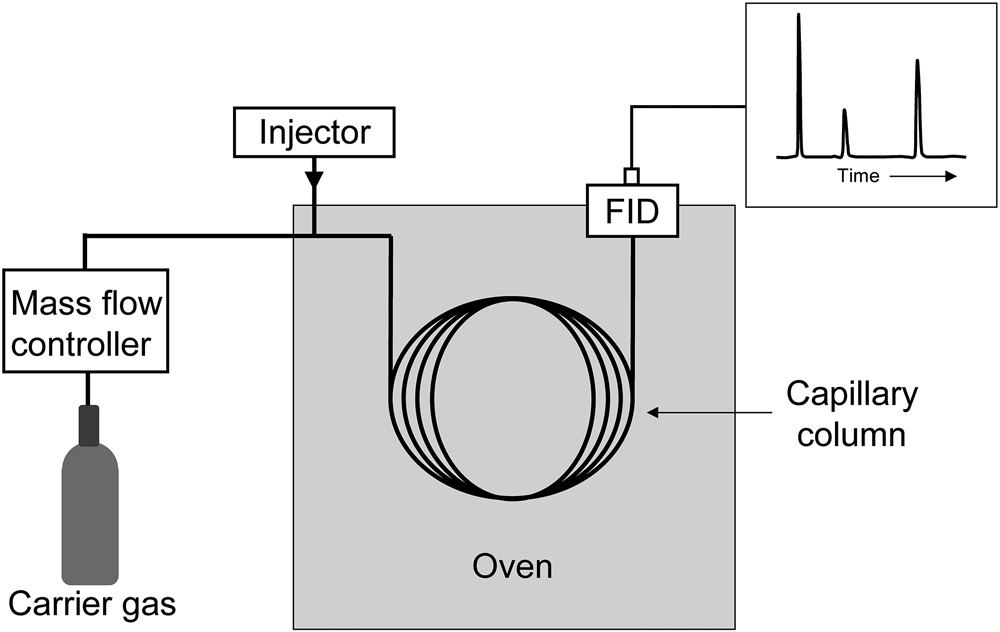
\includegraphics[width=0.6\linewidth]{pics/gc.png}
    \caption{Schematic diagram of a GC instrument. Courtesy of Chris Mayhew \cite{ellis2013proton}.}
    \label{fig:gc}
\end{figure}

\subsection{Ion Mobility Spectrometry}
In ion mobility spectrometry (\acrshort{ims}) ions are separated according to their mobilities through a gas. The typical experimental setup is shown in figure \ref{fig:ims}. An IMS device consists of three main parts: a cathode (radioactive source), where the reagent ions are generated; a drift tube, where an electric field drags the ions downstream; and a Faraday plate that detects the ions. The outcome is a spectrum that shows the signal versus drift time plot. Peaks in the spectrum can be assigned to compounds by knowing their mobilities. As a general rule, the lighter the ion, the higher its mobility, although other characteristics like its structure can affect the mobility as it influences how it interacts with the buffer gas. 

As in PTR-MS, the reagent ion used in IMS is usually hydronium and although radioactive sources are the most common ones, others like corona discharge and photoionisation sources are becoming more popular. The ions enter the drift tube when the gate that separates the ion source and the drift tube allows to do so. Also, the drift tube in IMS is similar to that in PTR-MS, as it will be explained later. Briefly, it consists of a series of stacked metallic rings alternated with insulator rings. Each of the metallic rings has a different electric potential in order to create a uniform electric field along the revolution axis. This dragging electric field together with the collisions with the background gas make the ions reach the so-called drift velocity.

Some of the advantages of IMS are that it is quite cheap, small and does not need big pumps as it works at a pressure similar to the atmospheric one. Due to this this technique is nowadays widely used in security and military applications – it can be often found in the security checks in airports, for instance. Moreover, its sensitivity is better than that of GC and can detect concentrations as low as 1 part per billion by volume (ppbv), allowing this technique to be used for real time measurements without pre-concentration. On the other hand, as GC does, IMS lacks good selectivity, being many compounds difficult to be completely separated and identified.

\begin{figure}%[h]
\centering
    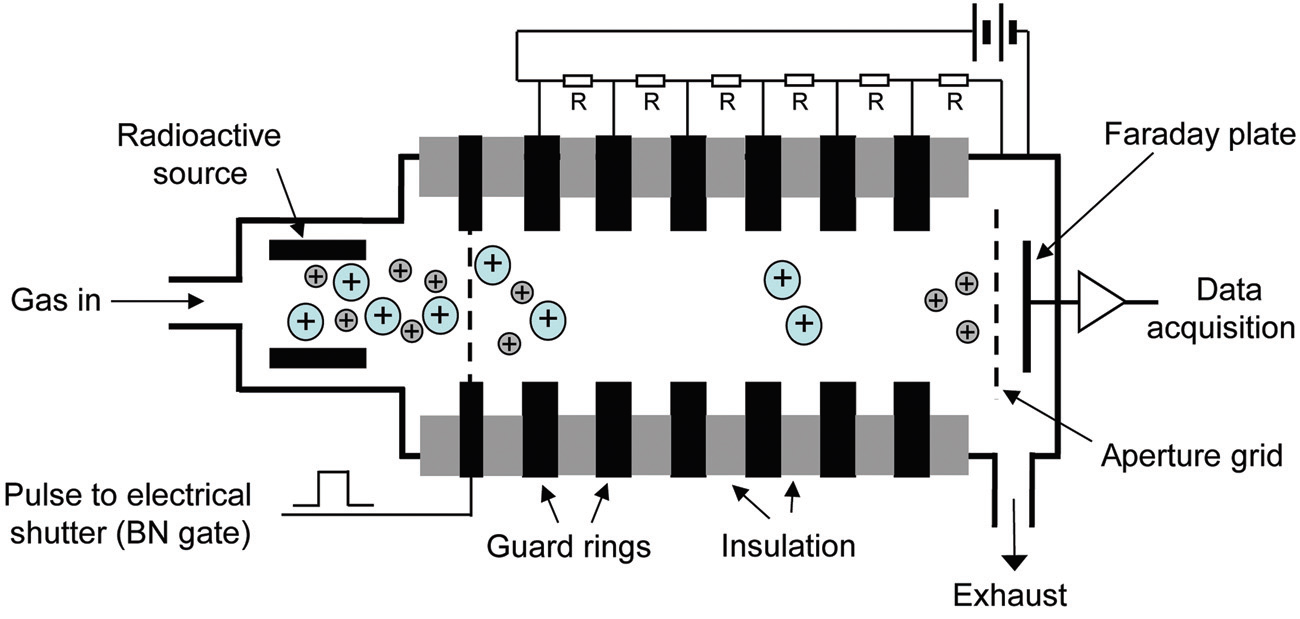
\includegraphics[width=0.7\linewidth]{pics/ims.png}
    \caption{Schematic diagram of an IMS instrument. Courtesy of Chris Mayhew \cite{ellis2013proton}.}
    \label{fig:ims}
\end{figure}

\subsection{Selected Ion Flow Tube}
Unlike IMS, selected ion flow tube mass spectrometry (\acrshort{sift}) does not use a drift tube, but a flow tube, to drag the ions downstream. As shown in figure \ref{fig:sift}, a SIFT-MS instrument consist of an ion source, a quadrupole mass filter, a flow tube and a mass analyser.

The reagent ions are created in the ion source, usually by means of electric discharges or through a heated electron filament source. These reagent ions can be a mixture of species – H$_3$O$^+$, NO$^+$, O$_2^+$, etc.  The quadrupole mass filter then selects the reagent ion by its mass. This piece of equipment also allows fast switching among the reagent ions, which can be used to extract more information of the analyte through the study of its interaction with the different reagent ions. From the mass filter, the ions enter the flow tube. Here He is used as a carrier gas and it is also in the flow tube where the analyte gas is injected. Finally, the ions are detected in a mass analyser, typically a quadrupole mass spectrometer.

The presence of helium in the flow tube makes it possible to explore ion-molecule reactions at thermal energies. One of the main applications of SIFT-MS, as it was of flowing afterglow (the precursor of SIFT-MS and similar to it, but without a mass filter among other things), is the ability to measure reaction coefficients. This has allowed SIFT-MS to become a valuable tool in areas like atmospheric and interstellar chemistry.

\begin{figure}%[h]
\centering
    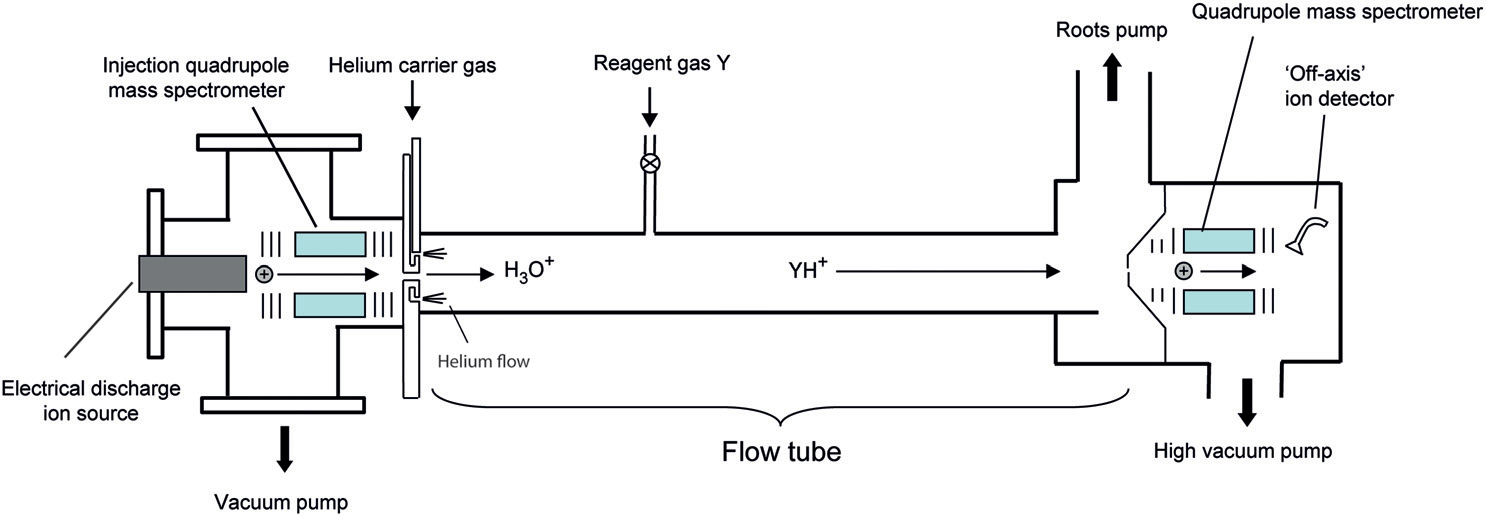
\includegraphics[width=0.8\linewidth]{pics/sift.png}
    \caption{Schematic diagram of a SIFT-MS instrument. Courtesy of Chris Mayhew \cite{ellis2013proton}.}
    \label{fig:sift}
\end{figure}



\section{The PTR-ToF-MS}
As stated in the introduction, PTR-MS is a sensitive technique for real-time monitoring of VOCs in air with a minimal sample preparation. PTR-MS uses hydronium as reagent ion to donate protons to the VOCs present in the analyte gas and detect trace concentrations of targeted compounds. This method was developed by Werner Lindinger at the University of Innsbruck (Austria) in the 1990 \cite{RN601} as the successor of the flowing afterglow  and the selected ion flow drift tube techniques. The newest PTR-MS instrument in our laboratory is shown in figure \ref{fig:littoral}. % and a schematic diagram is shown in figure \ref{fig:littoral_diagram}.
Briefly, the main  parts of a PTR instrument and their functions can be simplified to:
\begin{enumerate}
    \item Ion source: production of reagent ions.
    \item Drift tube:  protonation of the analyte.
    \item Mass spectrometer: detection of product ions.
\end{enumerate}
  These are explained in detail in the following sections.

\begin{figure}%[h]
\centering
\sidesubfloat[]{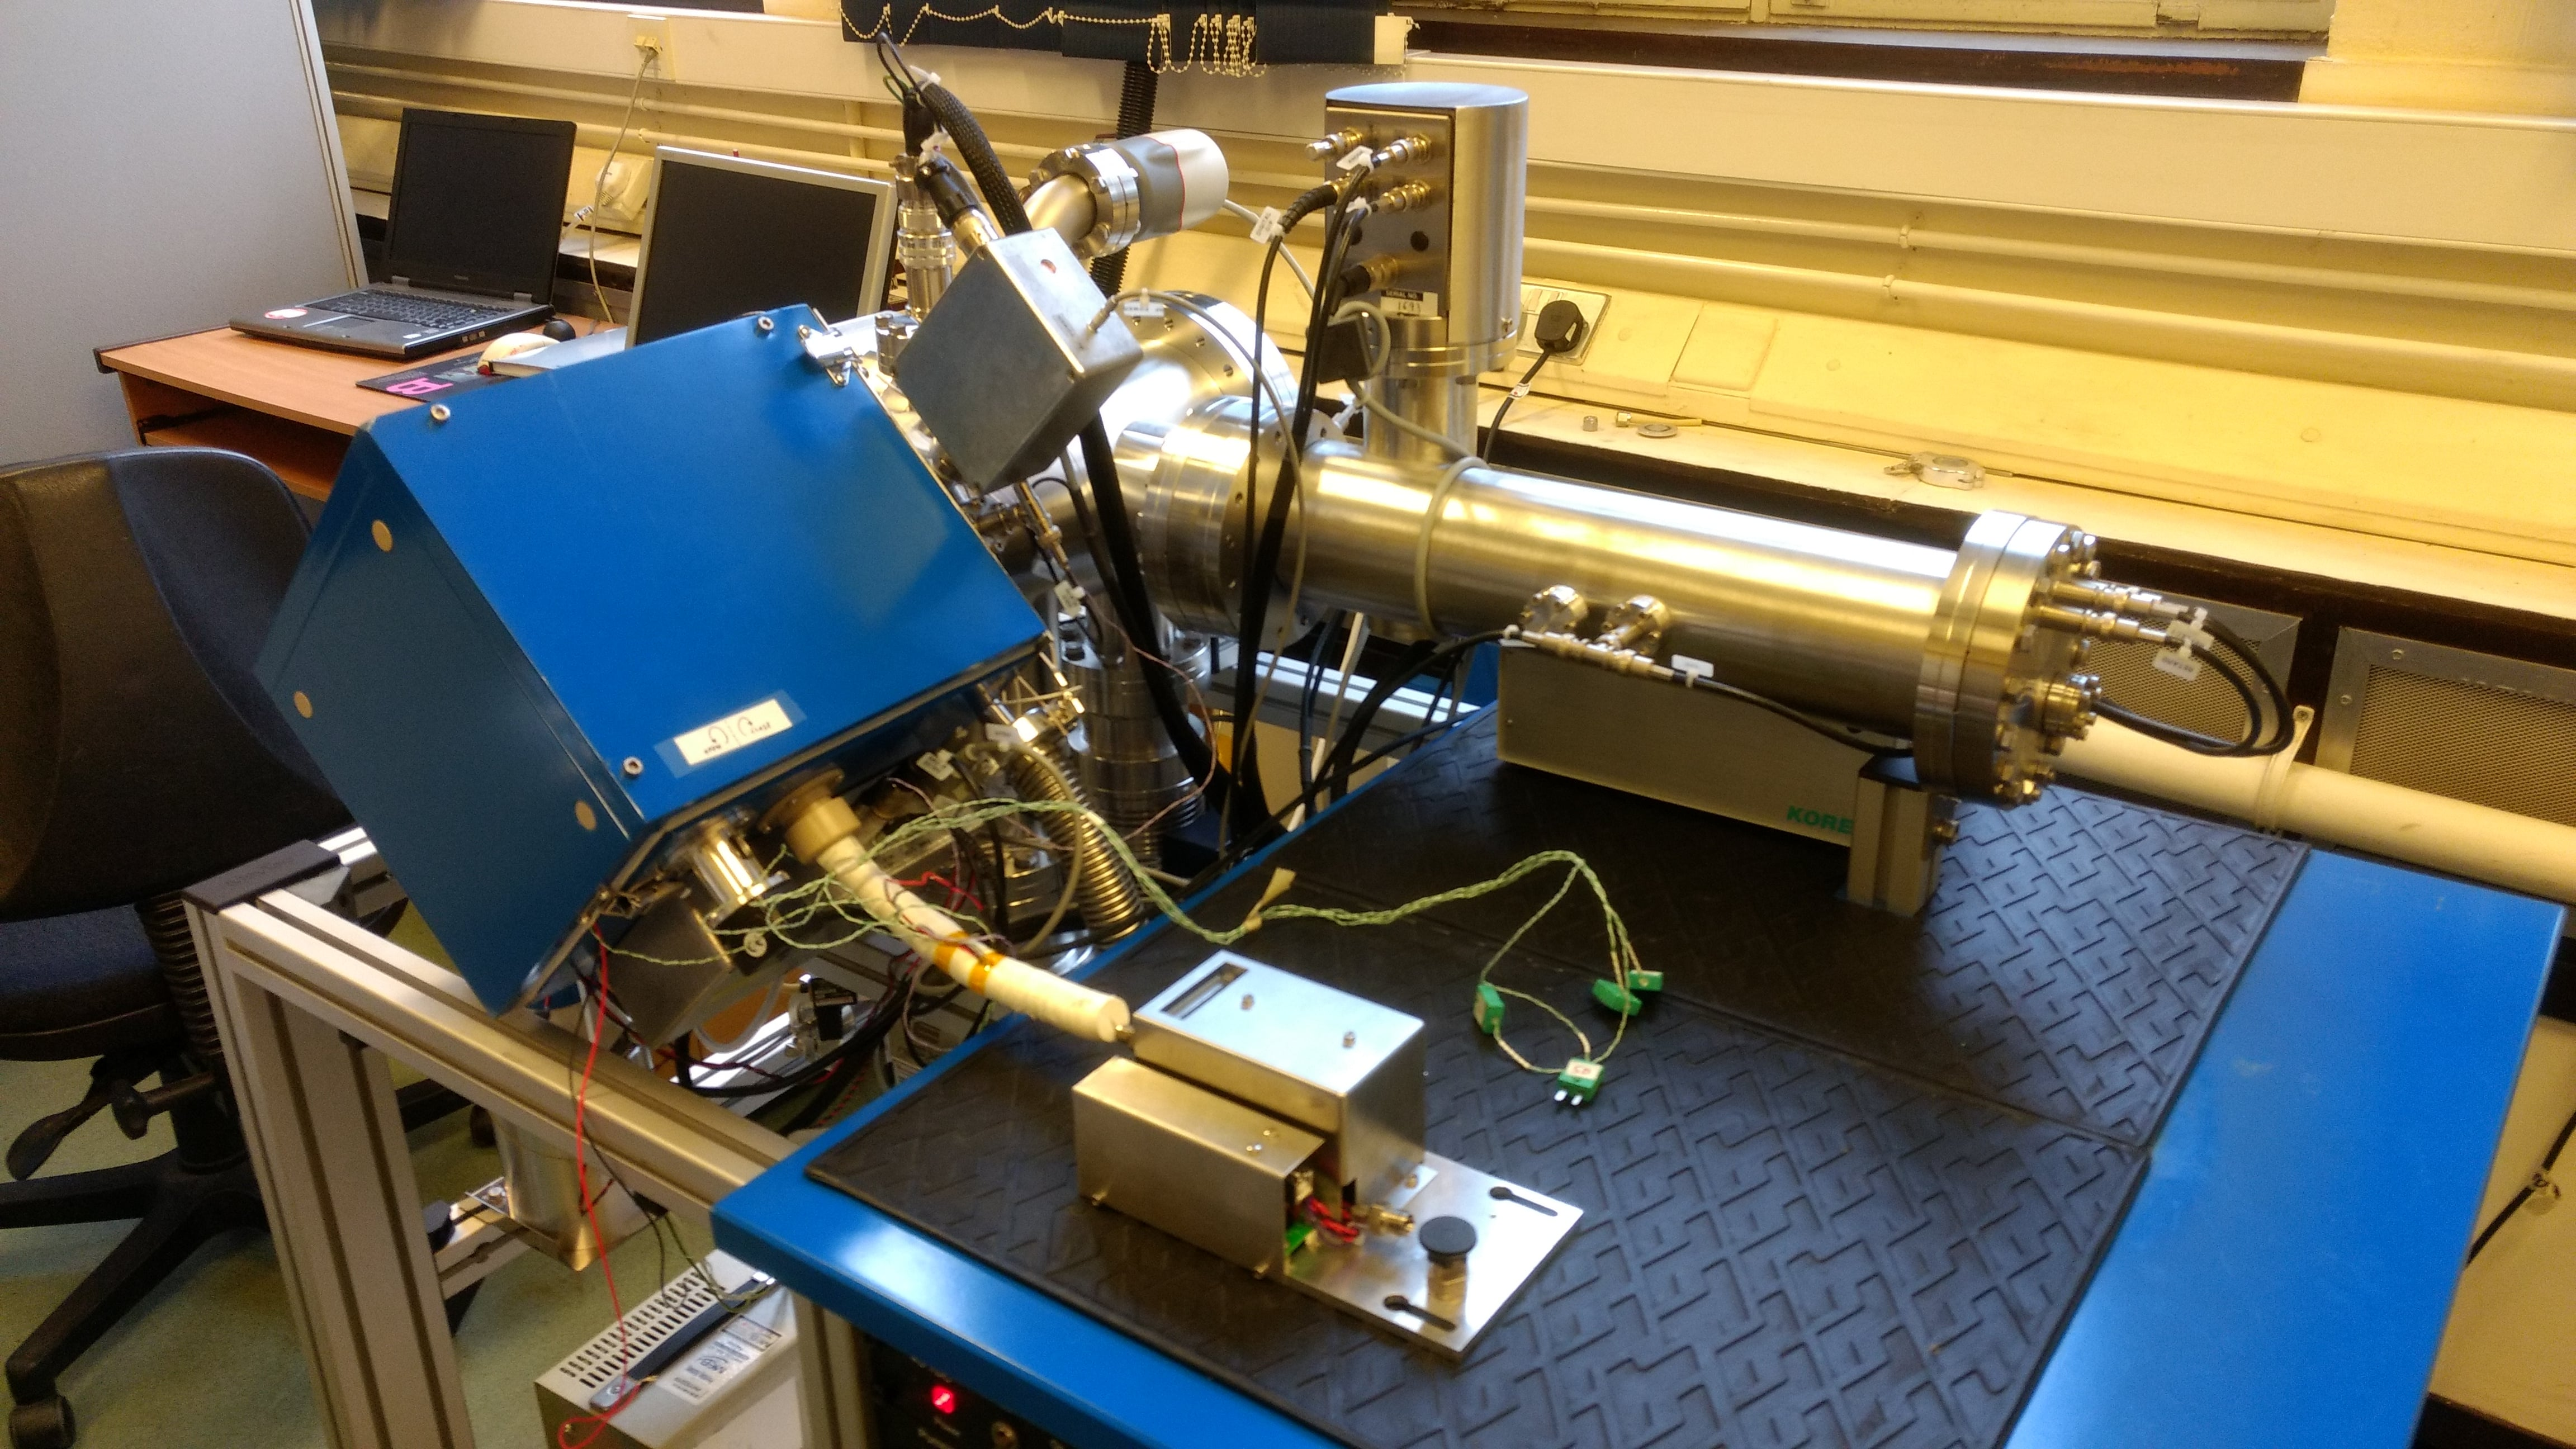
\includegraphics[width=0.9\linewidth]{pics/IMG_20170131_122756718}}

\bigskip
\sidesubfloat[]{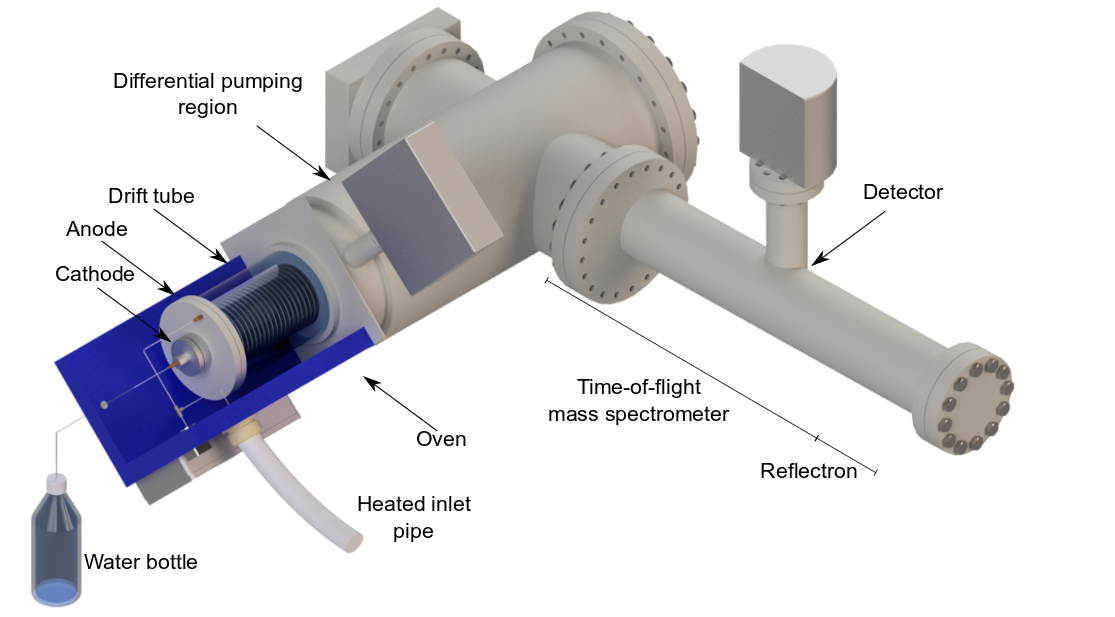
\includegraphics[width=0.95\linewidth]{pics/ptr-ilus.png}}
\caption{(a) Picture of a KORE Technology Ltd. Mk I RFIF-PTR-ToF-MS instrument.  (b) Illustration of the same PTR-ToF-MS instrument (not to scale) including the naming convention.}
\label{fig:littoral}
\end{figure}


% \begin{figure}
% \centering
% 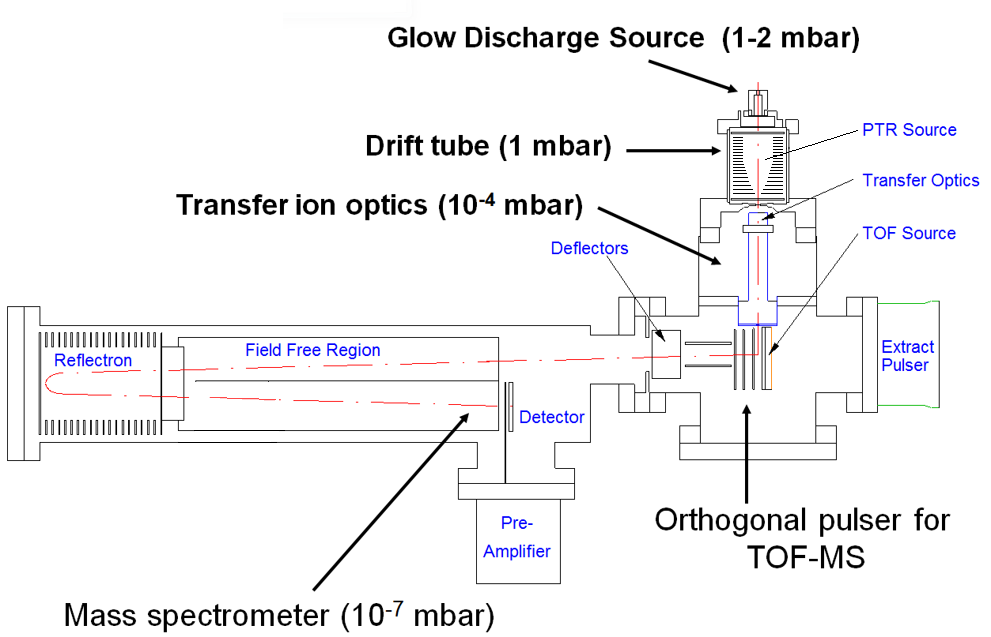
\includegraphics[width=0.8\linewidth]{pics/ptr_diagram.png}
% \caption{Schematic diagram of the main parts of a PTR-ToF-MS instrument. \textbf{ADD KORE LOGO}}
% \label{fig:littoral_diagram}
% \end{figure}

\subsection{Ion source}
The reagent ions that will ionise the sample are generated in the ion source. Most PTR-MS instruments carry a hollow cathode discharge ion source (see figure \ref{fig:cathode}), to which a voltage is supplied to ionise the gas that flows through it and create the plasma in which the reagent ions are being produced. The main advantage of a hollow cathode compared to a planar-electrodes ion source is that in the former higher ion densities can be achieved as the probability that ions hit the ion source's surface generating more ions is higher than in the planar electrode configuration. Note that the plasma in the ion source will be also referred to as the glow and the hollow cathode region as glow discharge (\acrshort{gd}).

\begin{figure}
\centering
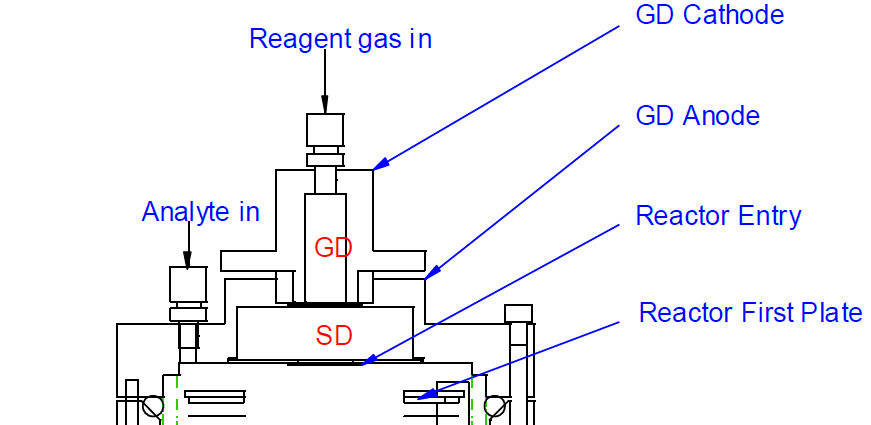
\includegraphics[width=0.8\linewidth]{pics/cathode.PNG}
\centering
\caption{Diagram of the hollow cathode of the PTR-MS apparatus manufactured by KORE Technology Ltd.}
\label{fig:cathode}
\end{figure}

\subsubsection{Experimental aspects}
During the standard use of the instrument, water vapour is supplied from the water reservoir to the cathode to generate hydronium ions. The pressure in the cathode can be adjusted by manipulating the valves that control the gas flow into the cathode and needs to be between 1 and 2 mbar, depending on the gas. Usually it is set between 1.3 and 1.4 mbar. Typically, the potential difference needed between cathode and anode to start the plasma in our instrument is approximately 750 volts. This is referred to as the breakdown voltage. An example of anode and cathode voltages in this configuration would be an anode voltage of 450 volts and a cathode voltage of -300 volts. The anode voltage floats with the voltage of the first plate of the drift tube, which can be adjusted by the user. After the plasma has started, the cathode voltage changes. The difference in voltage between the cathode and the anode is now the potential required to maintain the discharge, which is smaller than the breakdown voltage and it is usually between 350 and 400 volts.

After the glow discharge switch is turned on, it can take the plasma up to a couple of minutes to start. Increasing the pressure in the drift tube can assist to start the plasma, as some of the gas in the drift tube will be back-streamed into the cathode. If even with some back-streaming and setting the cathode at high pressure the plasma won't start, cleaning the ion source must be considered. An aluminium oxide layer forms inside the ion source and needs to be removed after some months of use. Another factor that affects the stability of the glow is the temperature of the oven that contains the ion source and the drift tube. We have experienced that the higher the temperature of the oven is, the higher the cathode pressure must be for the glow to be maintained.

\subsubsection{The glow discharge: production of reagent ions}
Glow discharge is a type of electrical discharge that occur at low pressures (mbar range) and is characterised by a maintained current of 1uA to 1A between the cathode and the anode. It receives this name because the ionised gas produces a shining glow whose characteristics depends on the nature of the gas, its pressure and the voltage applied.

The main reaction occurring in the ion source driving to the production of H$_3$O$^+$ from the electrical discharge of water vapour is the first one shown in table \ref{tb:reactions}. It starts when H$_2$O$^+$ has been produced through the electron impact (\acrshort{ei}) ionisation of water. However, other water fragment ions can also undergo reactions that generate hydronium, following the other reactions shown in table \ref{tb:reactions}. The rate coefficients at which these reactions happen show that they happen at the collision-limiting rate or very close.


\begin{table}[ht]
\centering
\caption{Chemical reactions through which hydronium can be produced starting from products of EI of water vapour and their rate coefficients at 300K \cite{doi:10.1002/rcm.1290030312}.}
\label{tb:reactions}
\begin{tabular}{ l l l }
\multicolumn{3}{l}{
$\begin{aligned}\toprule
\qquad H_2O^+ + H_2O 	&\rightarrow H_3O^+ + OH \qquad \qquad	& k = 1.8\times10^{-9}\, cm^{3}s^{-1} \qquad \\ \midrule 
OH^+ + H_2O  	&\rightarrow H_3O^+ + O  		& k = 1.3\times10^{-9}\,cm^{3}s^{-1} \qquad \\  
				&\rightarrow H_3O^+ + OH		& k = 1.8\times10^{-9}\,cm^{3}s^{-1}	 \qquad \\ \midrule
O^+ + H_2O  	&\rightarrow H_2O^+ + O  		& k = 2.6\times10^{-9}\, cm^{3}s^{-1}  \qquad \\ \midrule
H_2^+ + H_2O  	&\rightarrow H_3O^+ + H  		& k = 3.4\times10^{-9}\, cm^{3}s^{-1}  \qquad \\ 
				&\rightarrow H_2O^+ + H_2 		& k = 3.7\times10^{-9}\, cm^{3}s^{-1}	 \qquad \\ \midrule
H^+ + H_2O  	&\rightarrow H_2O^+ + H  		& k = 8.2\times10^{-9}\, cm^{3}s^{-1}  \qquad \\ \bottomrule
\end{aligned}$
} \\

\end{tabular}
\end{table}


Hydronium ions can cluster to water molecules via hydrogen bonds to form the so-called water clusters, i.e. (H$_2$O)$_n$H$_3$O$^+$ with n = 1, 2, 3 typically. Ideally, we want pure hydronium being injected into the drift tube. Otherwise, if the water cluster ions come into play, the reactions occurring in the drift tube can get too complicated to be properly understood. The instrument accommodates a source drift (\acrshort{sd}) region (see figure \ref{fig:cathode}) whose goal is to break the clusters apart before they enter the drift tube. If said clusters are not broken before entering the drift tube, they can also be split by increasing the collisional energy there.

\subsection{Drift tube}
The drift tube (\acrshort{dt}) is the region of a PTR-MS instrument where the protonation and possible fragmentation of the analyte occurs. Also, the DT is often referred to as the reactor. A picture of the DT is shown in figure \ref{fig:dt}.

\begin{figure}%[h]
\centering
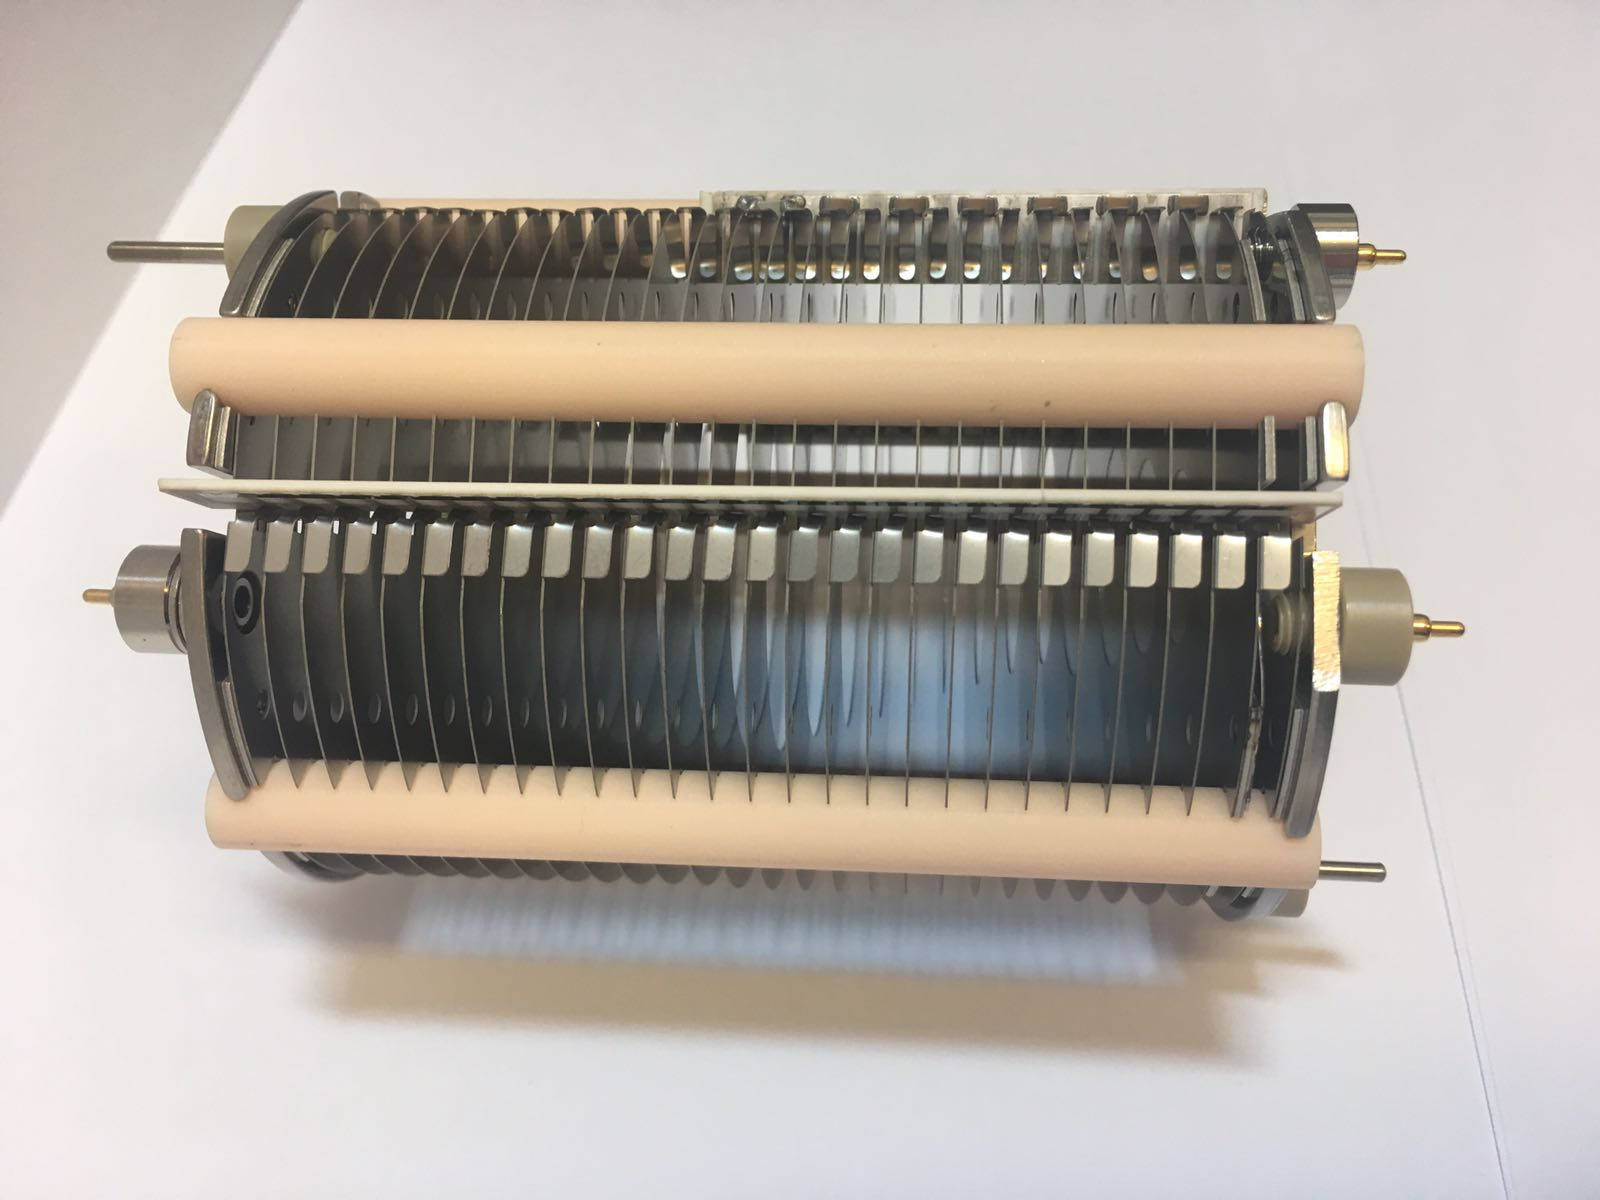
\includegraphics[width=0.8\linewidth]{pics/IMG-20170119-WA0008.jpg}
\centering
\caption[Picture of the drift tube of a PTR-MS instrument.]{Picture of the drift tube of a PTR-MS instrument. Note that in this model the diameter of the electrodes decreases in the second half of the stack.}
\label{fig:dt}
\end{figure}

\subsubsection{Experimental details}
Our main instrument is a KORE Technology Ltd RFIF Series 1 PTR-ToF-MS. Its drift tube, shown in figure \ref{fig:dt_diagram}, consists of 29 stainless-steel ring electrodes of 0.2 mm of thickness with a spacing of 3.2 mm per plate inside a cylinder of resistive glass. The inner diameter of these electrodes is 40 mm in the first half of the stack and it gradually decreases in the second half to 6 mm. A 1 M$\Omega$ resistor chain connected to the electrodes allows to supply a linearly decreasing potential to each of them when a voltage is applied between the first and the last plates, generating an electric field in the reactor known as DC field. When the instrument is operating in these conditions (i.e. without the RF field explained in section \ref{section:rfif}), we refer to it as working in DC mode or DC-only mode.

The DC electric field (see figure \ref{fig:dt_simion}) drags the ions across the reactor and towards the transfer lenses, where they will get transmitted into the mass spectrometer. As they are drawn through the reactor, ions collide with the neutrals molecules of the background and analyte gases, which can result in protonation and fragmentation of the analyte. The collisional energy can be manipulated by tuning the DC field as well as the reactor's pressure and temperature, whose standard values are around 1mbar and between 100 and 150$^{\circ}$C, respectively, although our oven can reach 200$^{\circ}$C. 


\begin{figure}%[h]
\centering
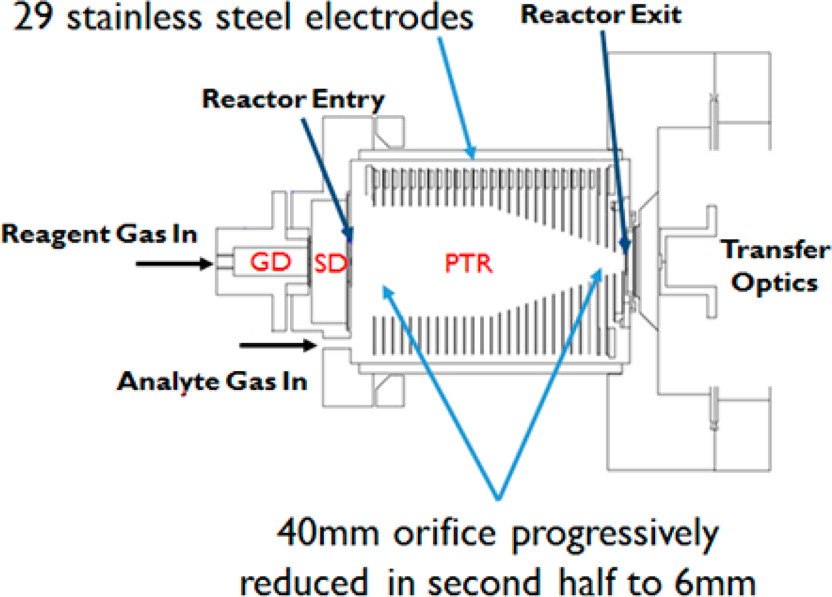
\includegraphics[width=0.6\linewidth]{pics/ac-2016-02982x_0002.jpeg}
\centering
\caption{Schematic diagram of the KORE Technology Ltd radio frequency ion funnel drift tube, together with the glow discharge and the source drift.}
\label{fig:dt_diagram}
\end{figure}


\begin{figure}%[h]
\centering
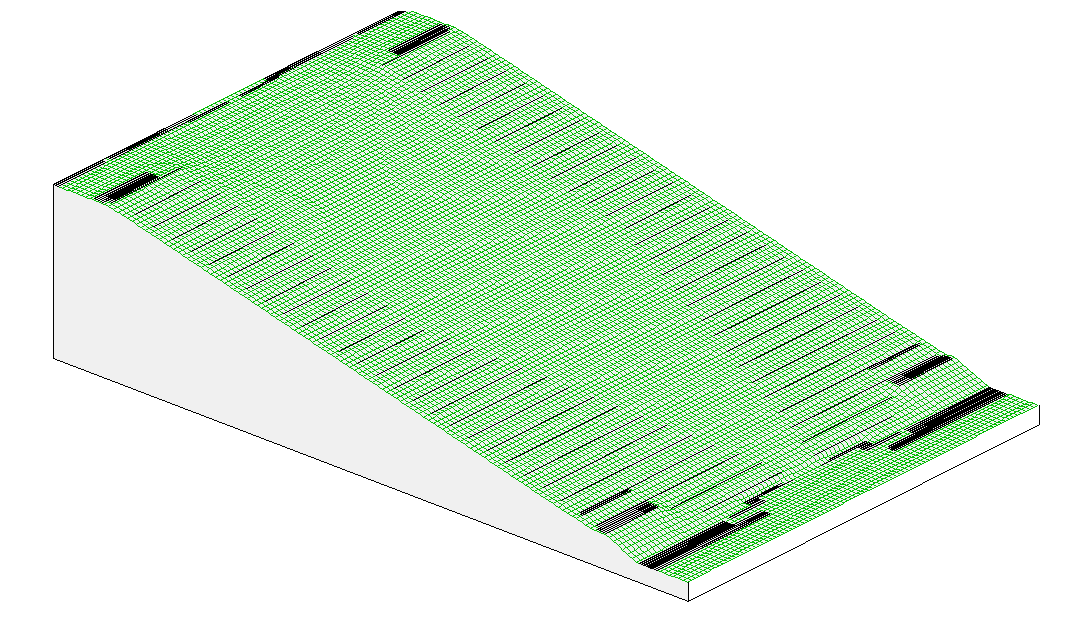
\includegraphics[width=0.8\linewidth]{pics/DC_SIMION.PNG}
\centering
\caption{Potential energy view of the cross section of the reactor in DC mode calculated in SIMION\textsuperscript{\textregistered}. The DC field gradient in this picture corresponds to 32 V/cm.}
\label{fig:dt_simion}
\end{figure}

\subsubsection{Reduced electric field}
As the collisional energy depends not only on the electric field, \acrshort{e}, but also on the buffer gas in the reactor, it is convenient to use the reduced electric field, \acrshort{en}, as a measure of the energy delivered to the ions. First, the electric field strength E is defined by the potential difference between the first and the last plate in the reactor divided by its length (equation \ref{eq:E}):
\begin{equation}
\lvert\vec{E}\rvert = \frac{V_d}{L}
\label{eq:E}
\end{equation}
where \acrshort{Vd} is the so-called drift voltage and it is equal to the voltage difference between the first and the last plate of the reactor, that can be adjusted by the user and are known as PTR Entry and PTR Exit, and L is the length of the drift tube, which is 9.36 cm in our newest instrument. For instance, a voltage difference between first and last plates of 300 V corresponds to an electric field of 32 V/cm.

Moreover, the gas number density, \acrshort{n}, is defined as the number of gas particles per unit volume and can be calculated from the ideal gas equation (equation \ref{eq:N}):
\begin{equation}
N = \frac{N_A}{V_{mol}}\frac{P_d}{P_0}\frac{T_0}{T_d}
\label{eq:N}
\end{equation}
where \acrshort{na} is the Avogadro's number (6.022$\times$10$^{23}$ mol$^{-1}$), V$_{mol}$ (22414 cm$^{3}$ mol$^{-1}$) is the molar volume of an ideal gas at standard temperature and pressure conditions, \acrshort{p0}  and \acrshort{t0}, T$_d$ is the temperature of the drift tube in Kelvin and P$_d$ is the gas pressure in the drift tube in mbar. For the standard operations conditions 1 mbar and 100$^{\circ}$C, N is 1.94$\times$10$^{16}$ cm$^{-3}$. The ratio E/N in this case would be 32 V cm$^{-1}$/1.94$\times$10$^{16}$ cm$^{-3}$ = 1.65$\times$10$^{-15}$ V cm$^{2}$. However, it is usual to express the reduced electric field in a different unit called Townsend (\acrshort{td}), which corresponds to 10$^{-17}$ V cm$^{2}$. Thus, 1.65$\times$10$^{-15}$ V cm$^{2}$ corresponds to an E/N value of 165 Td. Typically, a PTR-MS instrument is operated between 120 and 140 Td but going as low as 80 Td or as high as 240 Td is sometimes crucial to get a good picture of the dependence of the fragmentation with the collisional energy.

The ions inside the reactor reach a steady velocity, the so-called drift velocity, \acrshort{vd}, which is proportional to the electric field (equation \ref{eq:vd}):
\begin{equation}
\vec{v}_d = K\times \vec{E}
\label{eq:vd}
\end{equation}
where \acrshort{kk} is the ion mobility, which depends on the ion's mass and structure and the temperature and pressure in the reactor, and E the electric field in the drift tube. Note that the drift velocity does not represent the velocity of an individual ion but an average over the ion cloud. The drift velocity can be also be expressed in terms of the reduced mobility, \acrshort{kk0}, and the gas number density at standard pressure and temperature, \acrshort{n0}:
\begin{equation}
\vec{v}_d = K_0 N_0 \frac{\vec{E}}{N}
\label{eq:vd2}
\end{equation}
% where K and N are related to K$_0$ and N$_0$ through equations \ref{eq:k0} and \ref{eq:n0}:
% \begin{equation}
% K = \frac{P_0}{P_d}\frac{T_d}{T_0}K_0
% \label{eq:k0}
% \end{equation}
% \begin{equation}
% N = \frac{P_d}{P_0}\frac{T_0}{T_d}N_0			%I am not sure about this equation
% \label{eq:n0}
% \end{equation}


Besides the reduced electric field, the kinetic energy of the collisions in the centre-of-mass frame of reference, \acrshort{kecm}, can be used to characterise the ion-neutral collisions (equation \ref{eq:cm}):
\begin{equation}
\label{eq:cm}
KE_{CM} = \frac{m_n}{m_n + m_{ion}} \left( \frac{m_{ion}v_d^2}{2} + \frac{m_{b}v_d^2}{2}\right) + \frac{3}{2}k_BT
\end{equation}
where $\mu$ is the reduced mass of the system (equation \ref{eq:mu}), and m$_n$, m$_{ion}$ and m$_b$ are the masses of the of the neutral molecule (carrier gas), the reagent ion and the analyte molecule, respectively. Contrary to the reduced electric field, the centre-of-mass kinetic energy is mass-dependent and depends on the ions mobility through the drift velocity. The centre-of-mass is used rather than the lab reference frame as the proton transfer reactions are inelastic collisions because there is a transference of mass but still in the centre-of-mass reference frame the sum of the linear momentum of each of the molecules is equal to zero both before and after the collision (equation \ref{eq:cm2}):
\begin{equation}
\label{eq:cm2}
\sum_i \vec{p}_{i,CM} = 0
\end{equation}
However, the main challenge when using equation \ref{eq:cm} is to measure the drift velocity accurately enough. This has been done using the Hadamard transformation \cite{doi:10.1002/rcm.7254}.)
\begin{equation}
\label{eq:mu}
\frac{1}{\mu} = \frac{1}{m_n} + \frac{1}{m_{ion}}
\end{equation}

\subsubsection{Thermodynamics of proton transfer}
As mentioned before, the drift tube is where the protonation occurs. The reagent ions reach the drift tube by leaving the ion source through the anode aperture and passing by the source drift (SD) region, which helps to maximise the hydronium signal by breaking up the clusters. Once in the drift tube, they encounter the analyte gas, which is injected through the analyte pipe. The protonation occurs at the collisional rate if the proton affinity (\acrshort{pa}) of the analyte is higher than that of water (691 kJ/mol) following equation \ref{eq:pt}:
\begin{equation}
\label{eq:pt}
H_3O^+ + M \rightarrow MH^+ + H_2O
\end{equation}
where H$_3$O$^+$ is hydronium and M is the organic analyte of interest. 

Besides equation \ref{eq:pt}, protonation is also possible from the water clusters, if the PA of the analyte is higher than that of the n$^{th}$ water cluster, following equation \ref{eq:ptc}:
\begin{equation}
\label{eq:ptc}
(H_2O)_{n}H_3O^+ + M  \rightarrow MH^+ + (H_2O)_{n+1}
\end{equation}
where (H$_2$O)$_{n}$H$_3$O$^+$ denotes the n$^{th}$ water cluster ion. The PA of the water clusters is higher than that of the monomer. For example, the water dimer, (H$_2$O)$_{2}$, has a PA of 808 kJ/mol. Note that when the PA of the analyte is closer to that of the reagent ion the back reaction (equation \ref{eq:ptb}) can also occur:
\begin{equation}
\label{eq:ptb}
MH^+ + (H_2O)_{n+1} \rightarrow (H_2O)_{n}H_3O^+ + M 
\end{equation}





The PA of some compounds of interest are shown in table \ref{tb:pa}. One of the main advantages of PTR-MS is that ambient air can be directly sampled as its main constituents have smaller PA than water while most organic compounds of interest have a higher PA than that of water.

\begin{table}%[ht]
\centering
\caption{Organic compounds commonly found in air sorted by their proton affinity in kJ/mol \cite{doi:10.1063/1.556018}.}
\label{tb:pa}
\begin{tabular}{lcc}
\toprule
\quad \textbf{Compound}	 &\textbf{Formula}	&\textbf{PA (kJ/mol)} \quad\\ \midrule 
Oxygen           & O$_2$     		& 421   \\
Hydrogen         & H$_2$     		& 422.3 \\
Nitrogen         & N$_2$    	 	& 465   \\
Nitrogen oxide   & NO     			& 531.8 \\
Carbon dioxide   & CO$_2$    		& 540.5 \\
Nitrogen dioxide & NO$_2$    		& 591   \\
\textbf{Water}            & \textbf{H$_2$O}    		& \textbf{684\footnotemark[2]}   \\
Formaldehyde     & CH$_2$O   		& 712.9 \\
Benzene          & C$_6$H$_6$   	& 750.4 \\
Methanol         & CH$_4$O   		& 754.3 \\
Acetic acid      & C$_2$H$_4$O$_2$ 	& 783.7 \\
Acetone          & C$_3$H$_6$O  	& 812   \\
\textbf{Water dimer}      & \textbf{(H$_2$O)$_2$} 	& \textbf{842\footnotemark[2]}   \\
\textbf{Water trimer}      & \textbf{(H$_2$O)$_3$} 	& \textbf{937\footnotemark[2]}   \\
\textbf{Water tetramer}      & \textbf{(H$_2$O)$_4$} 	& \textbf{1013\footnotemark[2]}   \\
\bottomrule
\footnotetext{\footnotemark[2]The proton affinity values for the water oligomers were calculated through quantum chemical calculations using the B3LYP functional and the 6-31+G(d,p) basis set by Peter Watts. %(See "Cocaine 24 07 18" from Peter Watts)
}
\end{tabular}
\end{table}

%\footnotetext{The proton affinity values for the water oligomers were obtained through quantum chemical calculations using the B3LYP functional and the 6-31+G(d,p) basis set. (See "Cocaine 24 07 18" from Peter Watts)}

The gas-phase basicity is the tendency of a compound to act as proton acceptor and it is equal to the negative Gibbs energy change of the protonation reaction in equation \ref{eq:pt}. Similarly, the proton affinity is the negative of the enthalpy change of a protonation process. Proton affinity and basicity (B) are related through equation \ref{eq:pa}:
\begin{equation}
\label{eq:pa}
PA = B - T\Delta S^0
\end{equation}
where T is the absolute temperature and $\Delta S^0$ is the entropy difference between reactants and products in the protonation reaction at standard conditions of pressure and temperature. If the PA of the analyte M is higher than that of water, i.e. PA(M) $>$ PA(H$_2$O), then the protonation of the analyte is an exothermic reaction and it is thermodynamically allowed. The fact that it is an allowed reaction does not say at what speed it will occur, but empirically it has been observed that proton donation occurs at a rate equal to the collisional rate, which means that a protonation will occurs in every collision.

The rate constant, k, of a protonation reaction is a second-order rate constant (units of cm$^3$/s), as it depends on the concentrations of two reactants, as shown in equation \ref{eq:k1}. This rate equation shows that the decrease of H$_3$O$^+$ with time is equal to the increase of MH$^+$ and that the reaction is governed by the concentration (in cm$^{-3}$) of the reactants and the rate constant. 
\begin{equation}
\label{eq:k1}
-\frac{d[H_3 O^+ ]}{dt} = \frac{d[MH^+]}{dt} = k[H_3 O^+ ][M]
\end{equation}

Assuming that the concentration of the analyte, [M] is much higher than that of the hydronium and that only a small proportion of the analyte is protonated equation \ref{eq:k1} can be integrated to get equation \ref{eq:k2}:

\begin{equation}
\label{eq:k2}
[MH^+] = [H_3O^+]\left(1-e^{-k[M]t}\right)
\end{equation}
where t is the reaction time (i.e. the time it takes the molecules to cross the drift tube). If the exponent of the exponential function is small, the Taylor expansion can be applied to equation \ref{eq:k2}.
The result is shown in equation \ref{eq:k3}.  This can be used to quantify the concentration of the analyte, [M], if the rate constant, the reaction time and the concentration of the protonated analyte and reagent ions are known accurately (assuming that the protonated analyte molecule is the only product ion).

\begin{equation}
\label{eq:k3}
\frac{[MH^+]}{[H_3O^+]} = -k[M]t
\end{equation}



% \paragraph{Dipole, collisional rate?}~\\
% Is this neccesary?

\paragraph{Charge transfer}~\\
Besides hydronium, other reagent ions can be produced in the hollow cathode. These can be either desired or undesired depending if we deliberately want to use a different reagent ion or if they are impurities, for example, when some gas is back-streamed from the drift tube. The most common reagent ions used in PTR-MS besides H$_3$O$^+$ are NO$^+$ and O$_2^+$. They are also the contaminants we usually struggle with, but if the ratio of intensities of NO$^+$ and O$_2^+$ with H$_3$O$^+$ are less than 1\% their influence in the measurements can be ignored. This can be easily achieved by running the experiments using N$_2$ as buffer gas instead of lab air.

Strictly speaking, with NO$^+$ and O$_2^+$ we must refer to the ionisation process as charge exchange or charge transfer rather than proton transfer. NO$^+$ has a first ionisation energy of 9.26 eV, which is 12.1 eV for O$_2^+$. This means that they can undergo charge transfer reactions with molecules with ionisation energies below 9.26 eV and 12.1 eV, respectively, and NO$^+$ can also undergo association  if charge transfer is not energetically allowed (see table \ref{tb:ct}). Note that collisions with a third body  Z   are required to remove some energy from the adduct formation to be stable. Adduct formation does not occur frequently in the case of O$_2^+$ as organic molecules' ionisation energies are generally in the range of 8 to 11 eV, which results in a considerable amount of energy deposited into the molecule that usually originates excessive fragmentation. In fact, for some molecules the mass spectrum resulting from charge transfer with O$_2^+$ as reagent ion is quite similar to the \acrshort{ei} spectrum, for which energies of 70 eV are commonly used. 

\begin{table}[ht]
\centering
\caption{Predominant reactions with NO$^+$ and O$_2^+$ as reagent ions.}
\label{tb:ct}
\begin{tabular}{l rl}
\toprule
Charge transfer from NO$^+$ & $NO^+ + M$&$\rightarrow M^+ + NO$
\\ \midrule 
Charge transfer from O$_2^+$ & $O_2^+ + M$&$\rightarrow M^+ + O_2$
\\ \midrule
Adduct formation with NO$^+$ & $NO^+ + M + Z$&$\rightarrow M.NO^+ + Z$  
\\ \bottomrule
\end{tabular}
\end{table}


\subsubsection{Radio frequency ion funnel}\label{section:rfif}
The Radio Frequency Ion Funnel (\acrshort{rfif}) is a novel piece of equipment developed by KORE Technology Ltd that both delivers extra collisional energy and focuses the ions towards the exit aperture of the drift tube, enhancing both sensitivity and selectivity of the PTR-MS instrument. As mentioned in earlier sections, in the second half of the drift tube stack the electrode's diameter gradually decreases from 40 mm to 6 mm in a funnel-like arrangement. The suitable electronics to provide these funnel electrodes with an RF field are mounted in the instrument. These electronics 
%consist of a RLC circuit that 
provide the second half of the drift tube's electrodes with a signal of 760 kHz and 200 V peak-to-peak in resonance that we will refer to as RF field (see figure \ref{fig:rfif_simion}). At any given time, adjacent funnel plates are supplied with an RF field of opposite polarity. Also, this RF field can be turned on and off in the front panel of the instrument and when it is superimposed to the DC field, which is always on, we say the instrument is operating in RF mode. Furthermore, in RF mode we do not use the reduced electric field, E/N, to refer to the collisional energy as in this mode the electric field is not uniform in the drift tube.

\begin{figure}%[h]
\centering
%\sidesubfloat[]{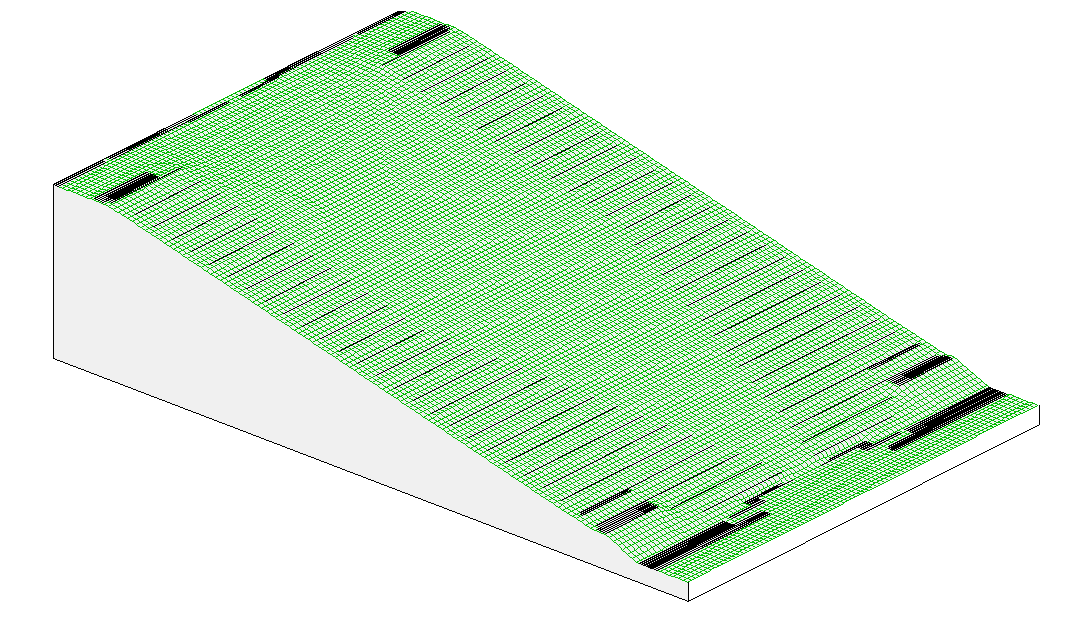
\includegraphics[width=0.8\linewidth]{pics/DC_SIMION.PNG}}\\
%\sidesubfloat[]{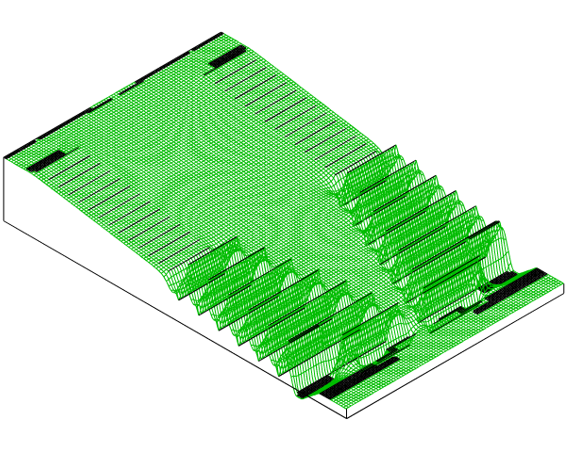
\includegraphics[width=0.8\linewidth]{pics/RF_SIMION.PNG}}
%\centering
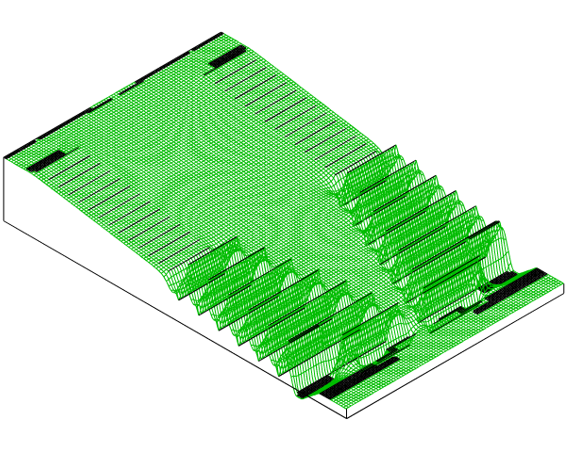
\includegraphics[width=0.8\linewidth]{pics/RF_SIMION.PNG}
\caption{Potential energy view of the cross section of the reactor in RF mode modelled in SIMION\textsuperscript{\textregistered} with a DC field gradient of 32 V/cm. Contrary to figure \ref{fig:dt_simion}, this is a snapshot as the RF field is time dependent.}
\label{fig:rfif_simion}
\end{figure}

\subsection{Differential pumping region and transfer lenses}
When the ions leave the drift tube through the exit plate's orifice, which has a diameter of 400 $\mu$m, they enter the differential pumping region, where the transfer lenses are. There is a pressure drop from the 1 mbar range in the drift tube to the 10$^{-4}$ mbar range in the differential pumping stage. This translates into a change in the type of flow, from viscous flow in the drift tube to a molecular flow in the transfer lenses region and further downstream in the mass analyser. This means that the mean free path of the ions gets bigger than the dimensions of the chamber, up to tens or hundreds of meters, and thus ion-wall collisions are predominant over ion-neutral or ion-ion collisions.

The aim of the transfer lenses is to focus the ion beam and transport it to the mass spectrometer. For this purpose, the ion beam is driven through a set of ring electrodes at different voltages. These ion optics focus the ions in the centre of a pinhole in the same way optical lenses do with light. The pinhole helps to clean the beam from chromatic aberrations, which translates into narrower peaks in the mass spectra because the ion beam that reaches the mass analyser is less spatially spread out (figure \ref{fig:tl_simion}). Also, two pairs of deflectors (not included in figure \ref{fig:tl_simion}) can be tuned to steer the beam to maximise the transmission into the mass spectrometer. 

It is important to note that a high potential gradient between exit plate and the first transfer optics electrode can help to increase the transmission but can create a hard extraction of ions. In the case of a hard extraction, ions are uncontrollably being fragmented beyond the exit plate in the early stages of the transfer optics, where the density of ions is still high. This undesired fragmentation can be avoided by setting  the electric field between the exit plate and the first electrode in the transfer optics to a few V/cm.

\begin{figure}%[ht]
\centering
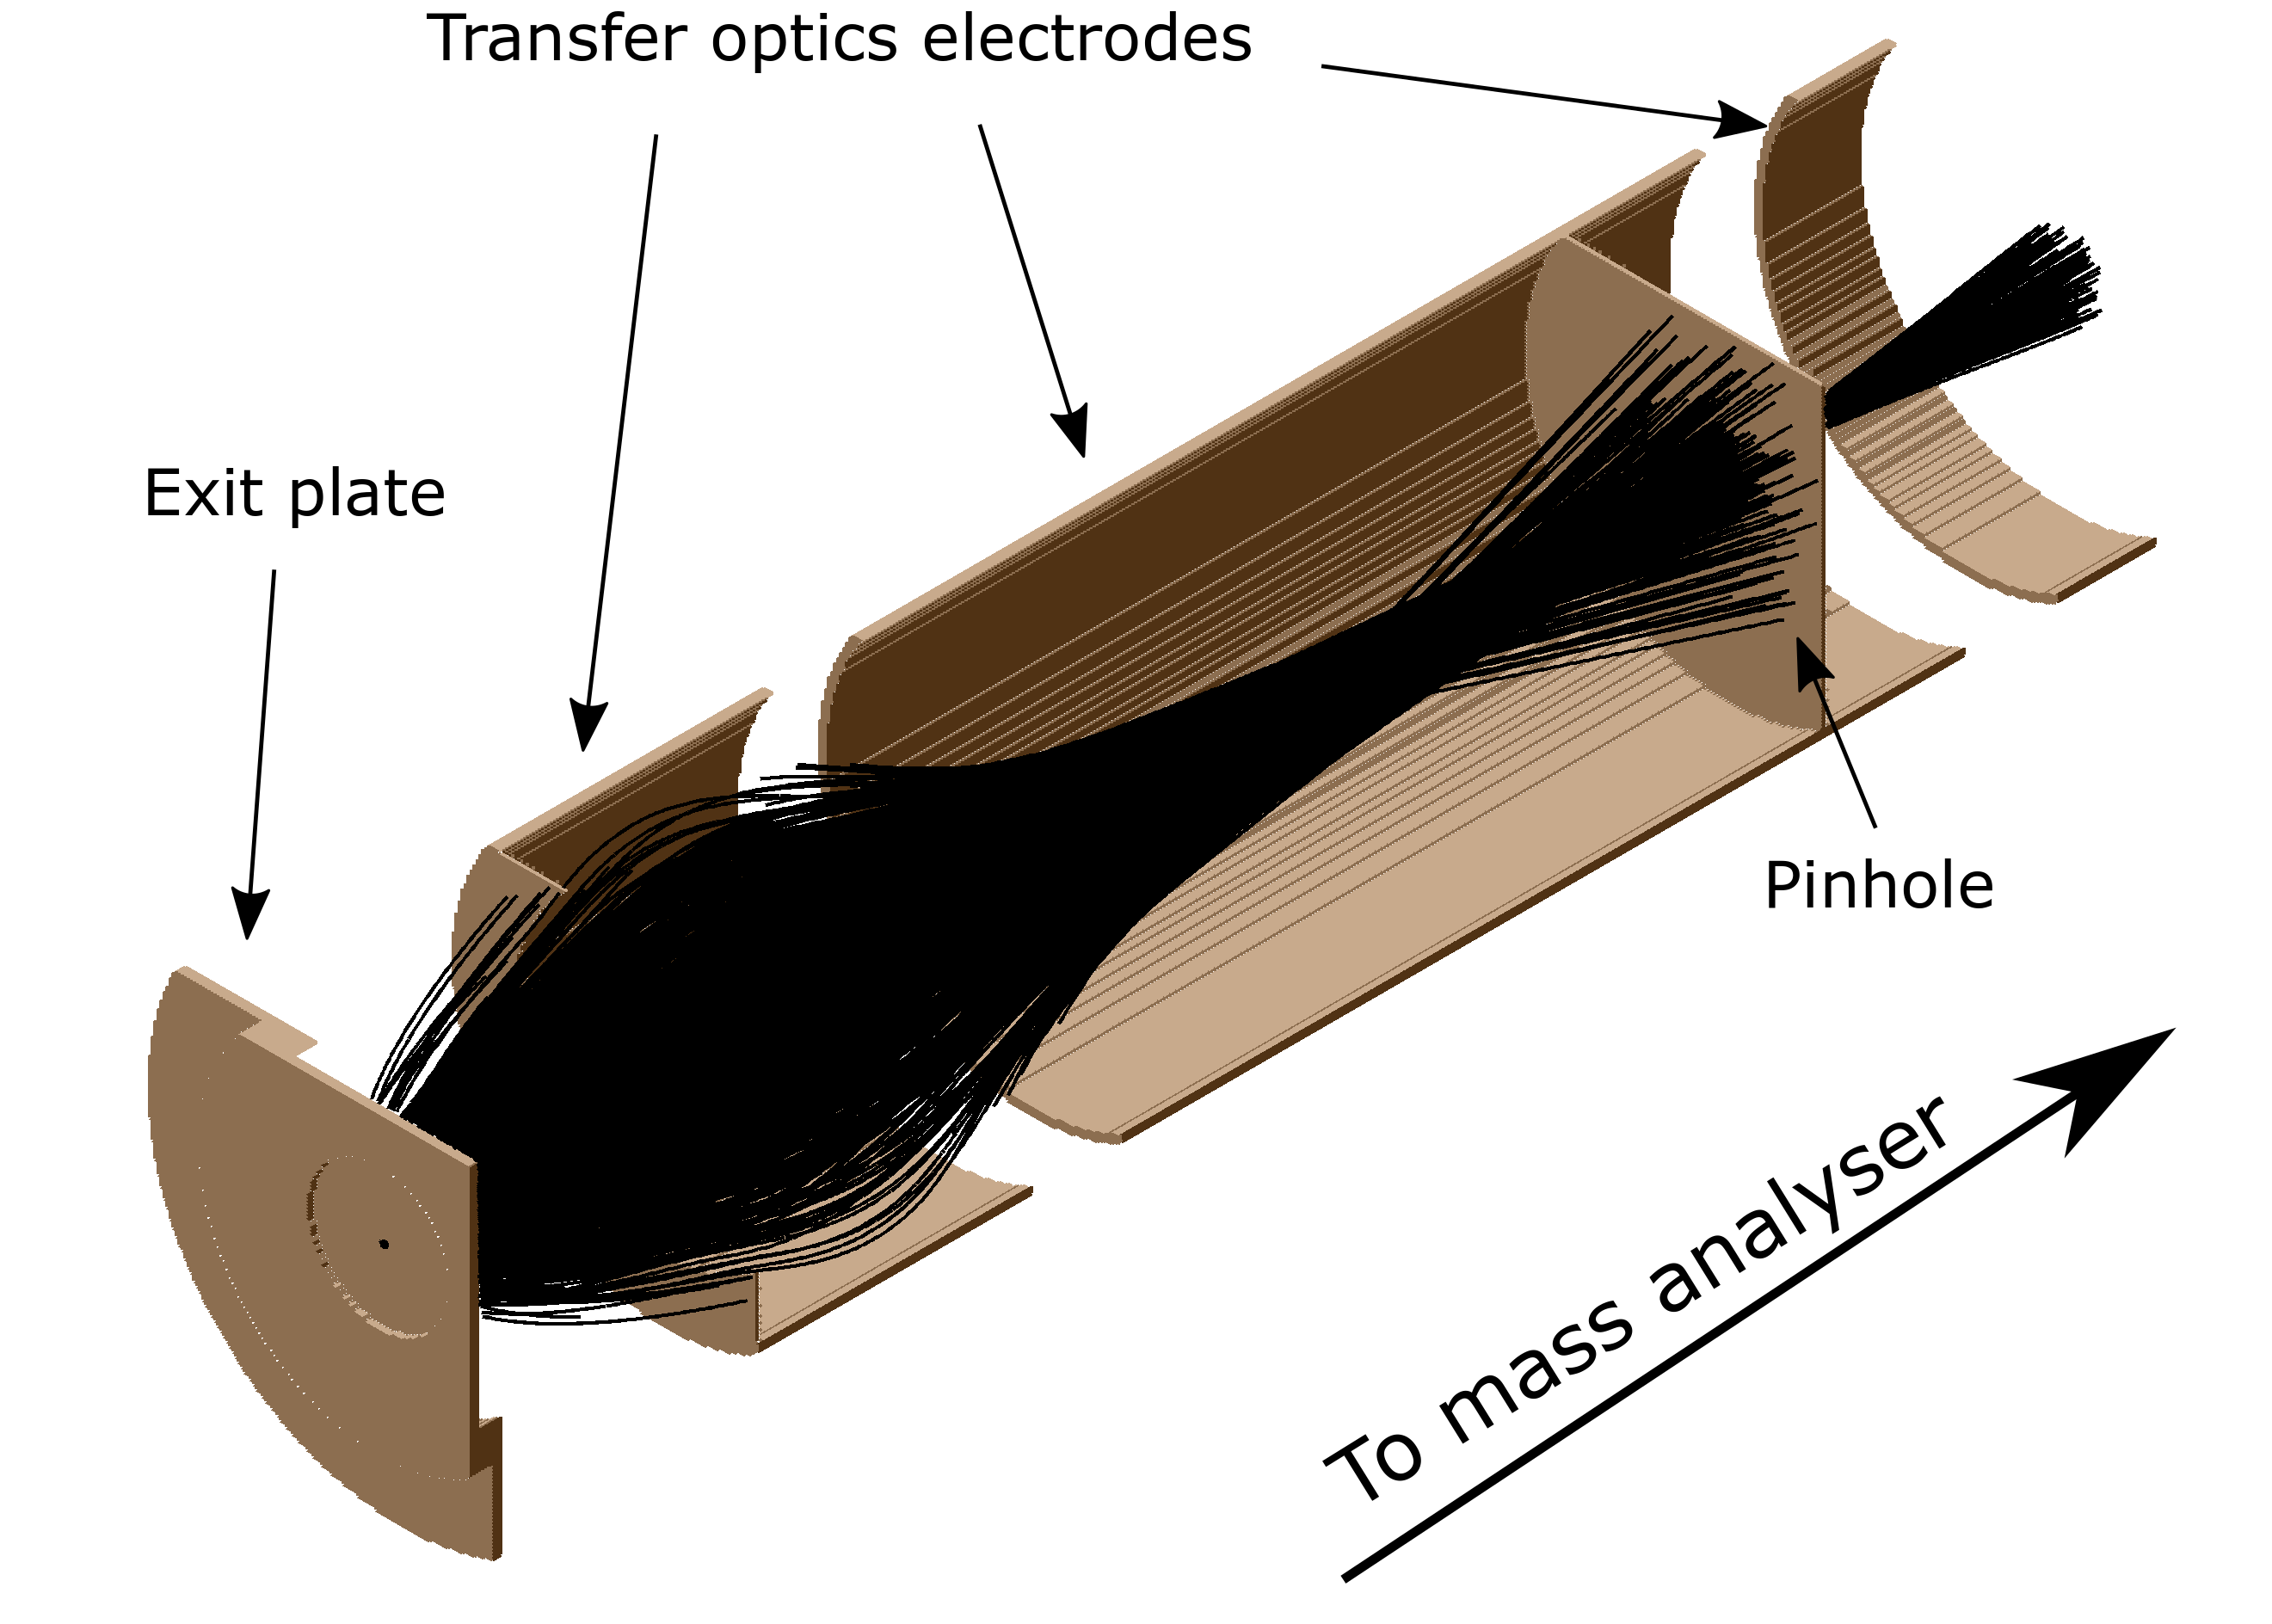
\includegraphics[width=0.8\linewidth]{pics/tf_names.png}
\centering
\caption[Simulation of the ion trajectories in the transfer lens region using SIMION\textsuperscript{\textregistered}.]{Simulation of the ion trajectories in the transfer lens region using SIMION\textsuperscript{\textregistered}. 1000 ions of m/z 100 with kinetic energies uniformly distributed between 0 and 1 eV were flown.}
\label{fig:tl_simion}
\end{figure}


\subsection{Mass spectrometer}
The ion beam is transferred from the drift tube to the mass spectrometer (\acrshort{ms}) via the transfer optics. The MS detects the ions according to their mass-to-charge ratio and allocate them in a histogram-wise plot called spectrum. This task requires a vacuum pressure in the flight tube less than 10$^{-7}$ mbar.

The mass to charge ratio is abbreviated to m/z and it refers to the ratio of the ions' mass divided by their charge. SI units are not used for m/z. For simplicity, atomic mass units (\acrshort{amu}) are used for the mass (1 amu = 1.66$\times$10$^{-27}$ kg) and the number of fundamental electric charges are used for the charge (1 e = 1.60$\times$10$^{-19}$ C). Depending on the mass resolution of the MS, m/z is can be given as an integer (nominal mass) or as a real number (monoisotopic mass).  

\subsubsection{Time-of-flight mass spectrometer}
The time-of-flight mass spectrometers  (TOF-MS, figure \ref{fig:tof})  are some of the most widely mass spectrometers used in PTR-MS. 

A TOF-MS works as follows: when ions reach the entrance of the MS (pulser region), a pulsed high voltage V of some kilovolts orthogonally repels them towards the other end of the flight tube. Lighter ions will gain more speed than heavier ions, which means that they will reach the detector faster. The time it takes an ion to reach the detector and its m/z are related by equation \ref{eq:tof2}, which comes from the energy balance in equation \ref{eq:tof1}. This allows to calculate the m/z and build the mass spectrum by measuring the ions' time of flight. 

\begin{figure}%[ht]
\centering
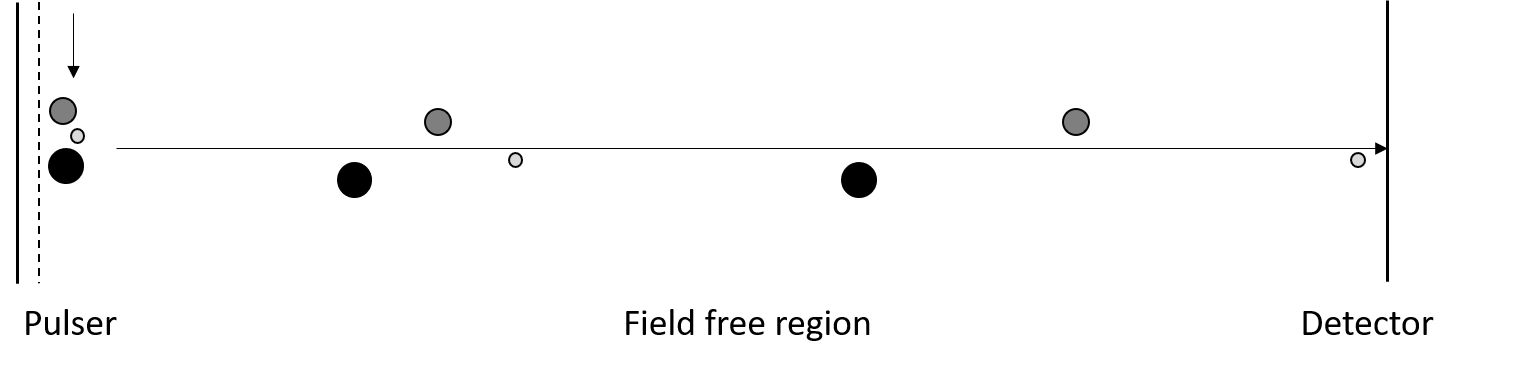
\includegraphics[width=0.8\linewidth]{pics/tofms.png}
\centering
\caption{Diagram of a linear time-of-flight mass spectrometer. Circles represent ions, being their diameter proportional to their mass-to-charge ratio.}
\label{fig:tof}
\end{figure}

\begin{equation}
\label{eq:tof1}
qV =  \frac{1}{2} m\left(\frac{l}{t}\right)^2
\end{equation}
\begin{equation}
\label{eq:tof2}
t= \sqrt{\frac{m}{z} \frac{l^2}{2eV}}
\end{equation}
where m/z is the mass-to-charge ratio of the ion, $l$ is the length of the flight tube, t is the flight time and $q = e z$ is the ion's charge. The pulser in a TOF-MS usually pulses at a rate of tens of kHz. 

\subsubsection{Reflectron}
A spatial distribution in the flight tube's pulser region can result in ions with different velocities, even for ions of the same m/z. This translates into broaden peaks in the mass spectrum. To amend this a reflectron, shown in figure \ref{fig:tofr}, can be implemented in the TOF-MS.

A reflectron consists of a series of electrodes with increasing voltage that will reverse the trajectory of the ions. When a cloud of ions reaches the reflectron, ions of the same m/z but going faster go deeper in it, having a longer flight distance than slower ions. This way, slow and fast ions will reach the detector at the same time. Narrower peaks and therefore improved mass resolution are achieved.

\begin{figure}%[ht]
\centering
%\sidesubfloat[]{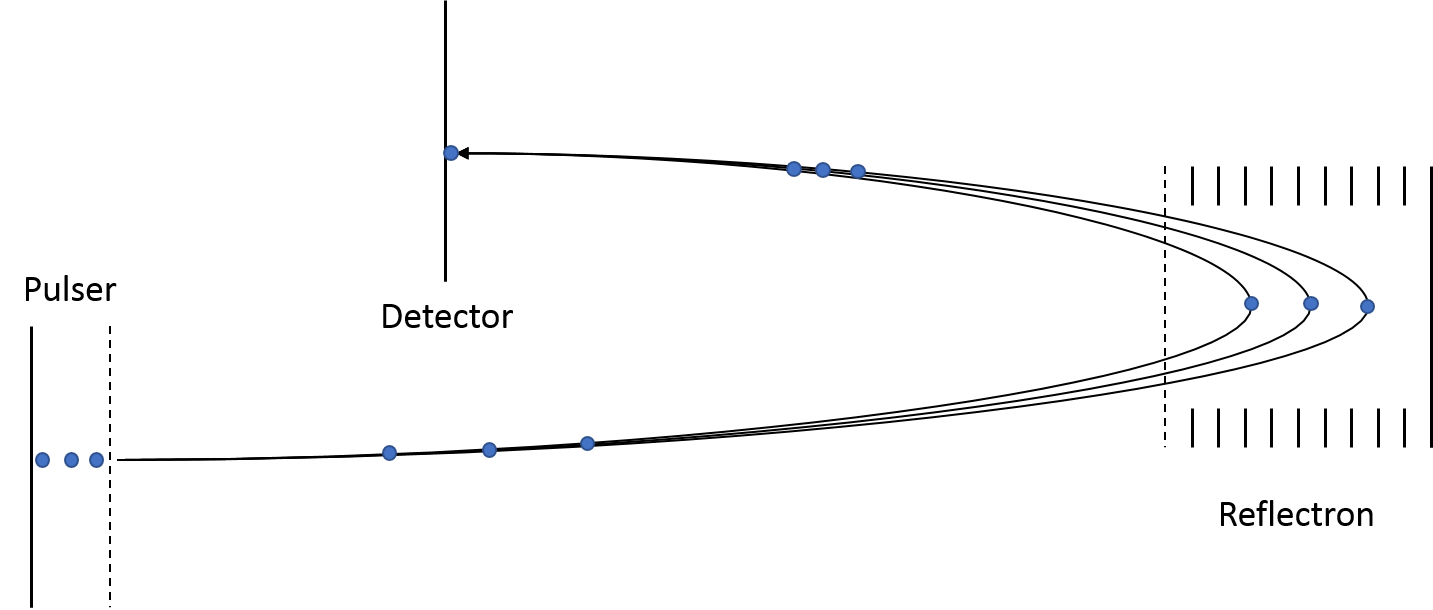
\includegraphics[width=0.8\linewidth]{pics/reflectron.png}}\\
%\sidesubfloat[]{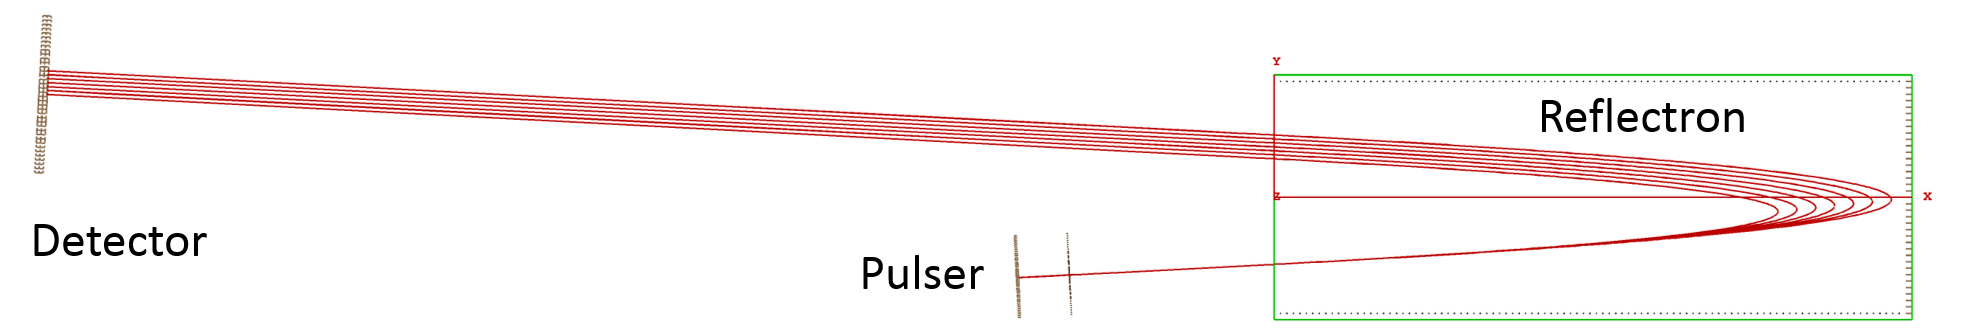
\includegraphics[width=0.8\linewidth]{pics/reflectron2.png}\label{fig:tofr_sim}}
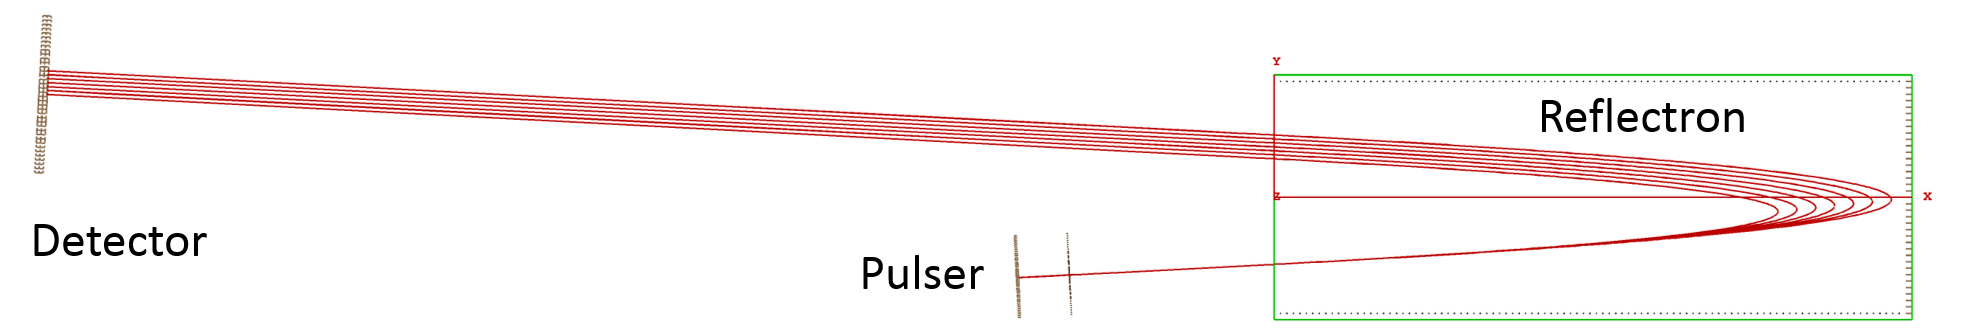
\includegraphics[width=0.8\linewidth]{pics/reflectron2.png}\label{fig:tofr_sim}
\caption{Schematic diagram of a flight tube with a reflectron showing the trajectory of  ions of the same m/z with different initial velocities.
}
\label{fig:tofr}
\end{figure}


\subsubsection{Detector}
Prior to detection, the ion signal needs to be amplified. A common pre-amplification setup consists of two microchannel plates (MCP) whose holes form an angle (figure \ref{fig:det}). With this arrangement no ion can go through without hitting the plates and creating a cascade. The MCPs are made of a material with a secondary electron emission greater than one, so that when the incoming ion hits it, more electrons are emitted, generating an avalanche that can amplify a single event by up to a factor of 10$^8$. The amplified signal will reach then the anode. Afterwards, the time-to-digital converter (TDC) will process the analogue signal in the anode and convert it into a digital one.


\begin{figure}%[ht]
\centering
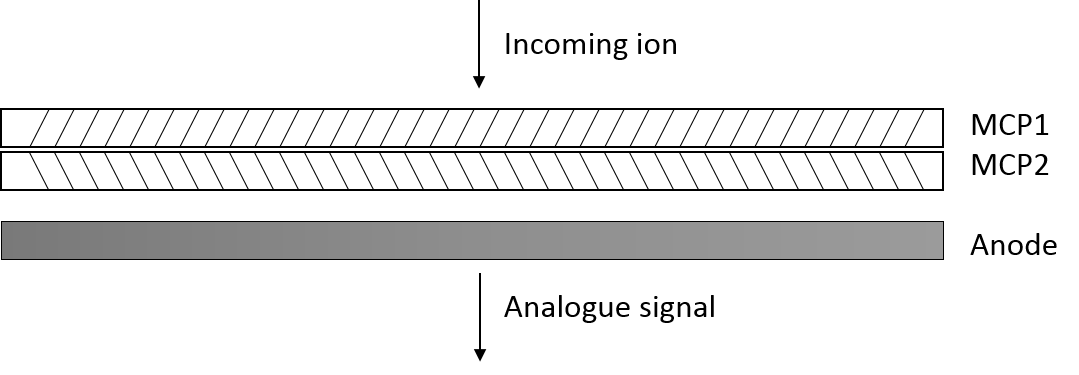
\includegraphics[width=0.6\linewidth]{pics/mcp.png}
\centering
\caption{Schematic diagram of a MCP detector.}
\label{fig:det}
\end{figure}

\subsubsection{Time-of-flight vs quadrupole}
A quadrupole can also be used as mass filter. It consists of four parallel rods (see figure \ref{fig:quad})  from which opposite rods will be at the same electric potential. Said potential is a combination of static and time-dependent fields for which only ions of a certain mass-to-charge ratio will have a stable trajectory. This allows to select the m/z we want to filter, and these ions will reach the detector at the end of the quadrupole.

Compared to time-of-flight mass spectrometers, quadrupoles are more compact, robust and cheap. On the other hand, quadrupoles also have some disadvantages. By their principle of operation, quadrupoles need to do a mass scan to build up the mass spectrum. This makes them much slower than time-of-flight devices, which can take measurements in up to 200 ms and are therefore suitable for transient experiments like desorptions. Similarly, the mass resolution of quadrupoles doesn't allow to distinguish between isobaric compounds, which can be done using a time-of-flight mass filter. Also, there is an upper limit for quadrupoles' mass range, which in theory is not a problem in time-of-flight devices although a mass limitation can arise from the use of reflectrons.

\begin{figure}%[ht]
\centering
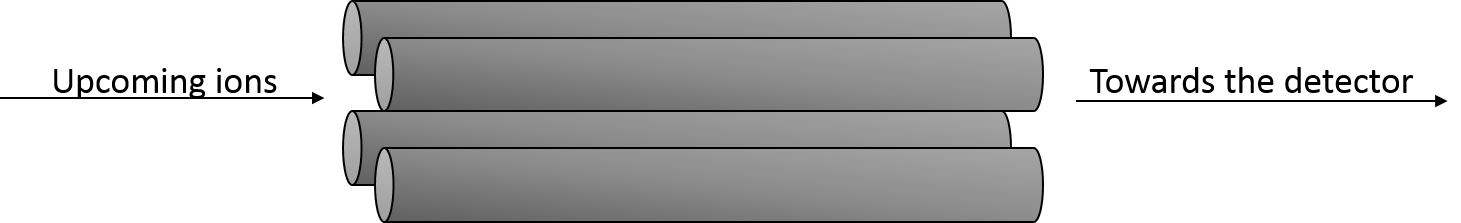
\includegraphics[width=0.8\linewidth]{pics/quad.png}
\centering
\caption{Schematic diagram of a quadrupole mass filter.}
\label{fig:quad}
\end{figure}

\subsubsection{Calibration}
As any other scientific instrument, the PTR-ToF-MS must be calibrated before performing any experiment. Note that in this section we refer to calibration as the method to calculate the mass conversions parameters, not the calibration to calculate a concentration from a signal in counts per second. The mass conversions parameters can be calculated by selecting some reference peaks and assigning them their exact m/z. Some peaks that can be used to calibrate the instruments are the $^{18}$O isotope of hydronium (H$_3$$^{18}$O$^+$, m/z 21.022), NO$^{+}$ (m/z 29.998), NO$_2^{+}$ (m/z 45.993) and protonated acetone ((C$_3$H$_6$O)H$^+$, m/z 59.050). It is also useful to use the analyte ion that will be measured as a calibration peak. The TDC uses equation \ref{eq:cal} for this task doing a least squares fitting.

\begin{equation}
\label{eq:cal}
m\slash z =  \left(\frac{t-t_0}{C_b}\right)^2 
\end{equation}
where m/z is the mass-to-charge ratio, t is the ion's time-of-flight, and t$_0$ and C$_b$ are parameters that depend in the mass range the instrument will measure and in some experimental quantities like the length of the flight tube. This equation is the same as equation \ref{eq:tof2} for t$_0$ = 0 and C$_b$ = $l/\sqrt[]{2eV}$.


%\subsubsection{Saturation: Poisson distribution}

%The counting electronics in the PTR-ToF-MS assumes that each pulse measured at the MCP corresponds to one ion. This can be not true if two or more ions arrive at the detector very close together and their analogue signals overlap so that the TDC translates it as a single event. This is known as saturation and happens more often when a high concentration of a compound is being measured.

%At a given m/z, the maximum number of counts per second the instrument can measure corresponds to the number of cycles per second of the mass spectrometer, which is the number of times the ions are pulsed per second. In other words, at a certain m/z only one ion per cycle can be measured. Therefore, a compromise must be found when the experiment is being designed to avoid situations of saturation while getting a proper signal. The number of cycles is the inverse of the cycle time, which is usually 30 to 40 us. For example, for a cycle time of 30 us, the number of cycles per second is 33333, or in other words, the pulsing frequency is 33.333 kHz.

%Figure \ref{fig:sat} shows the difference in real and measured counts if the probability of two ions arriving at the detector at the same time is given by the Poisson distribution function and considering that saturation means more than one ion arriving at the same time. When we are measuring a number of events equal to the number of cycles per second is unlikely that only one ion is arriving at the detector at a time, and the signal is highly saturated. 

%The analytical expression is:
%\begin{equation}
%\label{eq:sat}
%P(x) = 1 - e^{-x}
%\end{equation}


%\begin{figure}%[ht]
%\centering
%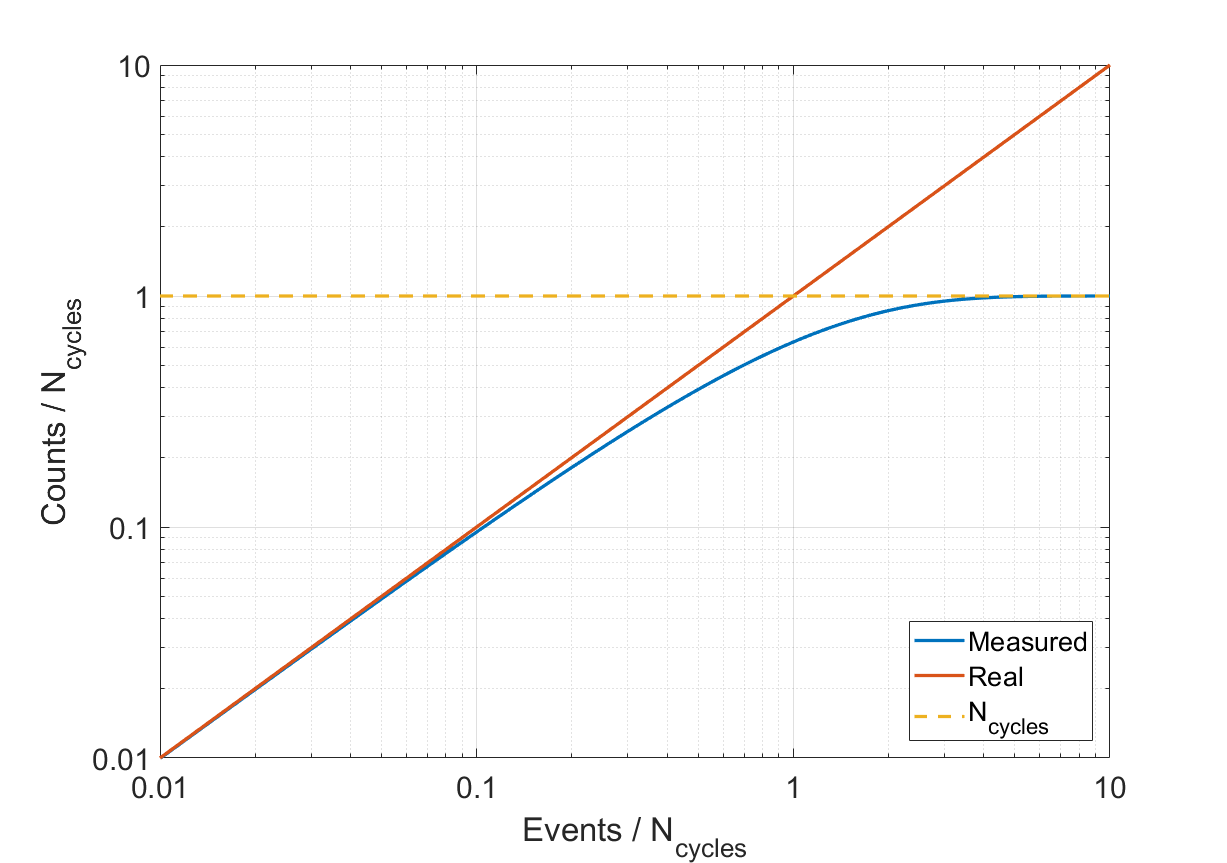
\includegraphics[width=0.8\linewidth]{pics/saturation.png}
%\centering
%\caption[Plot of the measured and real counts as a function of the number of events per cycle of the mass spectrometer.]{Plot of the measured (blue) and real (red) counts as a function of the number of events per cycle of the mass spectrometer. The dashed line corresponds to the number of cycles per second and indicates the maximum possible measured counts. Note that this plot is normalised to the number of cycles per second.}
%\label{fig:sat}
%\end{figure}






\section{Thermal Desorption Unit}
PTR-MS has been proved a sensitive tool for many applications, yet in homeland security the main technique in the market is \acrshort{ims}. Most substances of interest in this field, which include drugs and explosives, as well as in other areas have a low vapour pressure at room temperature, which make their detection challenging. These are often referred to as semi volatile organic compounds (\acrshort{svoc}). Swab desorptions into an IMS device are widely used and the same approach can be brought into PTR-MS. KORE Technology Ltd developed a thermal desorption unit (\acrshort{tdu}, figure \ref{fig:tdu}) that can be used in conjunction with a PTR-MS instrument to detect SVOCs. This has been applied to the detection of explosives reaching limits of detection (\acrshort{lod}) of nanograms \cite{RN445}.

The TDU works with polytetrafluoroethylene (PTFE) swabs mounted in a carboard frame onto which the targeted compounds are swept. Then, the swab is inserted in the TDU, whose plates come together clamping the swab and creating a seal. The plates are kept at high temperature and a carrier gas is flown through their holes, dragging the analyte towards the inlet pipe. 

%This creates a desorption profile like the one in figure REFFFFF, where the two main fragment ions from a 300 ng desorption of heroin are shown. It usually takes between 60 and 120 s for a sample to be completely desorbed into the instrument after the swab has been inserted in the TDU. After the measurement is finished, the TDU can be opened to extract the swab, which can be used again.

\begin{figure}
  \sidesubfloat[]{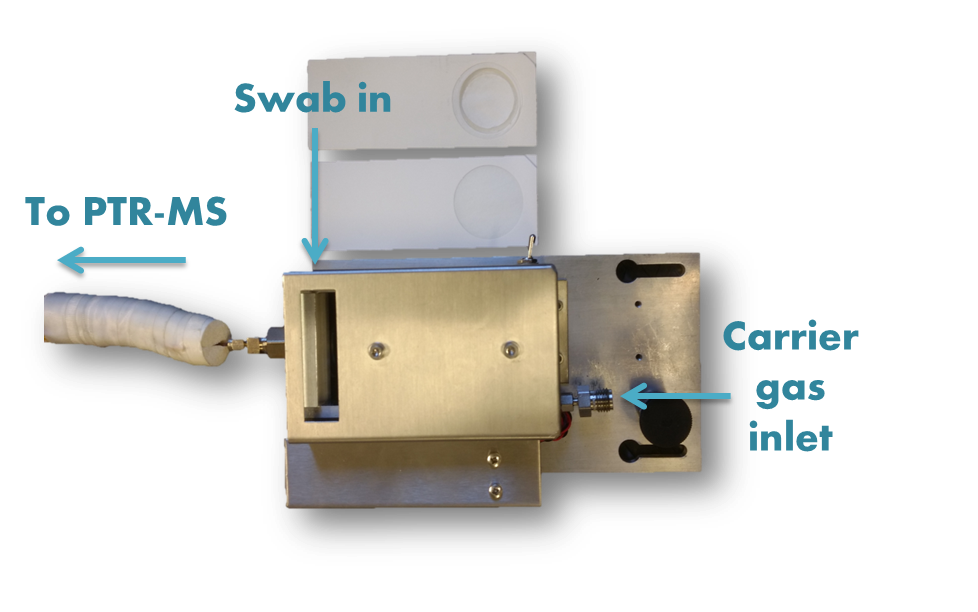
\includegraphics[width=0.8\linewidth]{pics/tdu.png}\label{fig:tdu1}}\\
  \sidesubfloat[]{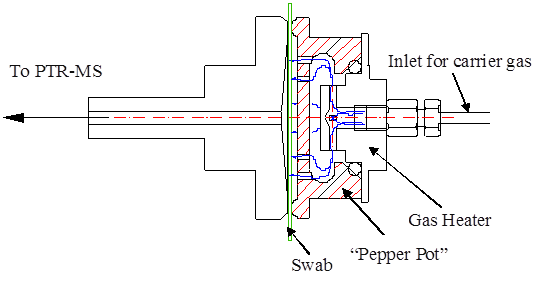
\includegraphics[width=0.8\linewidth]{pics/tdu2.png}\label{fig:tdu2}}
  \caption{(a) Picture of the TDU and its PTFE swabs. (b) Schematic diagram of the TDU.}\label{fig:tdu}
\end{figure}



%\section{Data analysis}

%\subsection{File specification}

%The analogue data recorded by the PTR-ToF-MS is translated into digital files by the time to digital converter (TDC) and can be visualised with the proper software. An experiment can consist in either a static or a transient measurement. Therefore, the data can be acquired either as a mass spectrum (.spc file) or as a temporal evolution of the mass spectrum (.lst file).

%A mass spectrum is the histogram plot of the counts (detected ions) as a function of their m/z which is stored in .spc files in our instrument. An example of a mass spectrum visualised with the Thermo Fisher Scientific  GRAMS/AI™ Spectroscopy Software is shown in Figure REFFFFF. The software does the time to m/z conversion following equation \ref{eq:cal}.


%On the other hand, the transient experiments can be stored in raw files called .lst files. These are binary files that record the timestamp of each event in three consecutive bytes in hexadecimal, with the most significant byte first. An event can be either the start of a cycle in the detector, always indicated by 0x000000, or a detected ion. This means that an .lst file holds all the information about the experiment. The software GRAMS/AI allows to open the .lst files as a mass spectrum (as that in Figure REFFFFF6) or as a chromatogram (Figure REFFFFF7), where the evolution of the m/z ranges of interest can be visualised. The latter is useful in conjunction with the TDU in the field of Homeland Security, as it will be explained in the results section.



% \subsection{Code for data analysis: Matlab\textsuperscript{\textregistered}}

% With a PTR-MS instrument a lot of data can be acquired easily so basic programming knowledge comes in handy when dealing with these big datasets. One of the best options is to use Matlab\textsuperscript{\textregistered} because some commands allow to easily open and manipulate Thermo Fisher's .spc files. Using this library as starting point, I wrote some code that extracts all the data from a study to analyse it in Matlab: measure peak positions, calculate counts, subtract background and assign possible chemical composition. This saves me lots of time :)





\section{Advantages and disadvantages of PTR-MS}
Some of the advantages of PTR-MS are:
\begin{itemize}
\item Specificity: PTR-MS can detect a large list of compounds such as aldehydes (like acetaldehyde), ketones (acetone), aromatic compounds (benzene), alcohols (methanol and ethanol), sulphur compounds (dimethyl sulfide), unsaturated compounds (isoprene), nitriles (acetonitrile) and esters. 
\item High sensitivity: limits of detection of parts per quadrillion by volume (ppqv) can be achieved \cite{ioniconlod}.
\item Little or no fragmentation of the ions, as compared to other ionisation mechanisms like electron impact.
\item Real time measurement:
\begin{itemize}
\item Fast reactions, with a rate coefficient close to the collision rate, in the order of magnitude of 10$^{-9}$ cm$^{3}$/s.
\item Direct sampling of atmospheric gases, which means that no sample preparation or pre-concentration is required.
\end{itemize}
\item Ease of operation, only requiring electrical power and distilled water.
\end{itemize}

On the other hand, PTR-MS also shows the following disadvantages:
\begin{itemize}
\item Water cluster formation and detection can interfere with the detection of other molecules. For instance, the $^{18}$O isotope of the first water cluster, (H$_2$O)H$_3$O$^+$, and the ion (C$_3$H$_3$)H$^+$ will  be both found at m/z 39. However, this issue can be solved with a high-resolution mass spectrometer and proper data analysis, i.e. using multi-peak fitting techniques or the isotopic distribution of the ions.
\item Inability to directly distinguish isomeric compounds. This can be mitigated by using tandem or fastGC techniques.
\item For compounds like benzene and toluene, which do not react with (H$_2$O)H$_3$O$^+$, the sensitivity depends on the humidity of the air, because higher humidity means higher concentration of (H$_2$O)H$_3$O$^+$ and lower of H$_3$O$^+$.
\item There exist some VOCs that don’t react with H$_3$O$^+$, like some alkanes, which have proton affinities below that of H$_2$O, so the back reaction (equation \ref{eq:ptb}) is not negligible.
\end{itemize}


\section{Applications of PTR-MS}
The ability of PTR-MS to detect and monitor trace concentrations of VOCs is advantageous in many fields. The main areas of application and some examples to illustrate them are:
\begin{itemize}
\item Atmospheric chemistry: 
\begin{itemize}
\item Determination of the emission of biogenic VOCs and their effect in the environment \cite{doi:10.1029/2003JD003863}.
\item Monitoring of pollution and urban plumes \cite{ROGERS200626}.
\end{itemize}
\item Homeland security:
\begin{itemize}
\item Detection of explosives \cite{GONZALEZMENDEZ201513,RN1254}, rape drugs \cite{doi:10.1002/jms.2993} and narcotics \cite{Agarwal2011}.
\end{itemize}
\item Medical sciences:
\begin{itemize}
\item Detection and monitoring of diseases through breath analysis \cite{FERNANDEZDELRIO20151243,doi:10.1152/jappl.2001.91.2.762,amann2014}.
\end{itemize}
\item Food sciences:
\begin{itemize}
\item Study of food aroma and flavour and quality control \cite{doi:10.1021/jf020922g,doi:10.1021/jf803998c,doi:10.1002/jms.1797}.
\end{itemize}
\end{itemize}





\chapter{%ENHANCEMENT OF SELECTIVITY IN 
PTR-MS AND ITS APPLICATIONS IN HOMELAND SECURITY% FOR THE DETECTION OF ILLICIT DRUGS
}
\markboth{PTR-MS  IN HOMELAND SECURITY }{}
 
 
\section{Introduction}
\section{Methodology}
 
\subsection{Reagent ion in DC mode and RF mode}
As stated before, proton donation to the targeted analyte comes from the collisions with the reagent ions, so it is crucial to monitor their signal to know the amount of available protons to be transferred to the analyte.

The signal of the hydronium and its clusters as a function of the drift tube voltage in both DC mode and RF mode is shown in figure \ref{fig:ri}. The $^{18}$O isotope peak is used to calculate the intensity of the reagent ions when their $^{16}$O peak is saturated. The natural composition of oxygen is $^{16}$O (99.76\%), $^{17}$O (0.03\%) and $^{18}$O (0.21\%) \cite{nistoxygen}.

The reagent ions' dependence with the voltage in DC mode is very different to that in RF mode. In DC mode the clusters break apart as the drift voltage increases. On the other hand, the RF field in RF mode delivers an extra collisional energy that breaks the clusters apart independently of the drift voltage. Also, this RF field can create potential wells for the lighter masses generating a low-mass cut-off of the transmission \cite{Chung123}.

The measured reagent ion signal depends on the clustering/declustering reactions and the transmission of the instrument. Furthermore, clustering depends on humidity, collisional energy (E/N) and drift time. The higher the pressure in the cathode, the more hydronium is produced but it also will tend to create hydrogen bonds with other ions. Moreover, the higher the collisional energy, the more collisions the clusters will undergo, making them dissociate eventually. And last, the longer the drift time, the more time the ions have to break apart through collisions.

\begin{figure}%[h]
\centering
\sidesubfloat[]{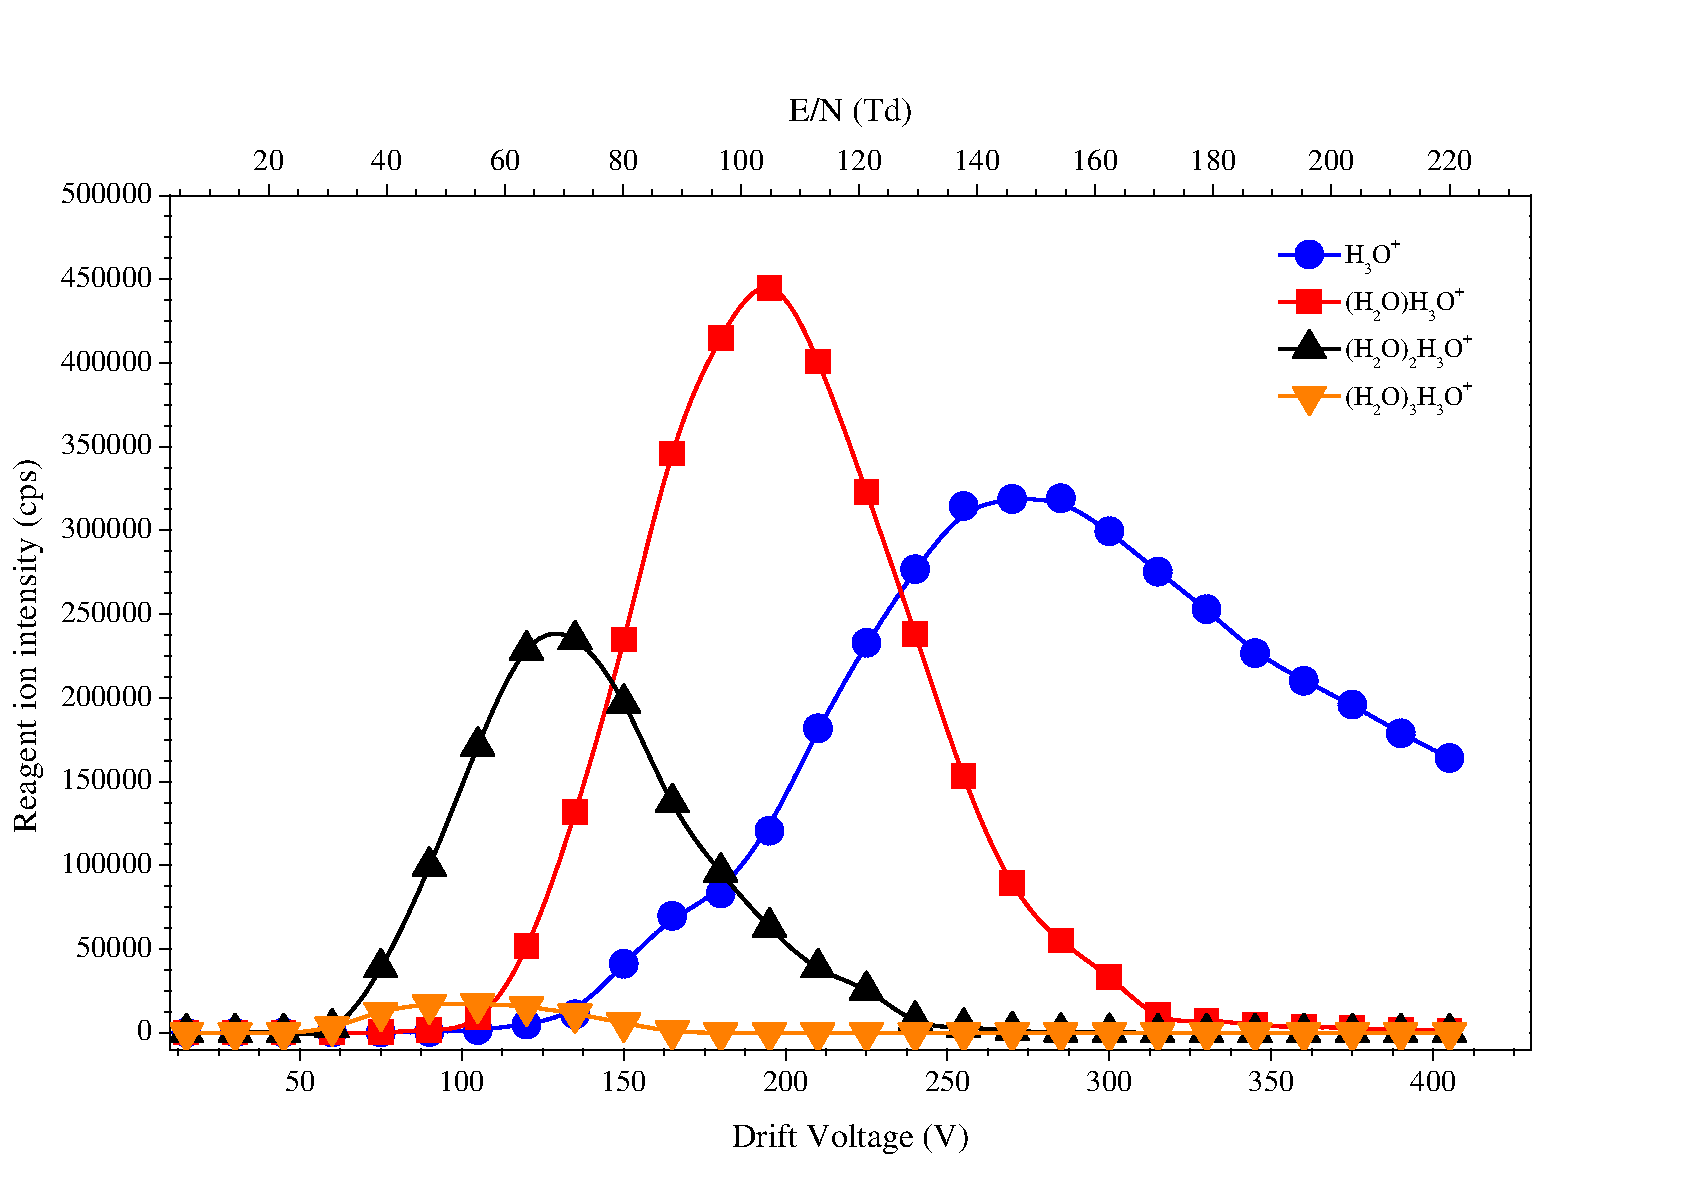
\includegraphics[width=0.8\linewidth]{pics/DPM_clusters_littoral.pdf}%water_DC.png}
\label{fig:ri1}}

\sidesubfloat[]{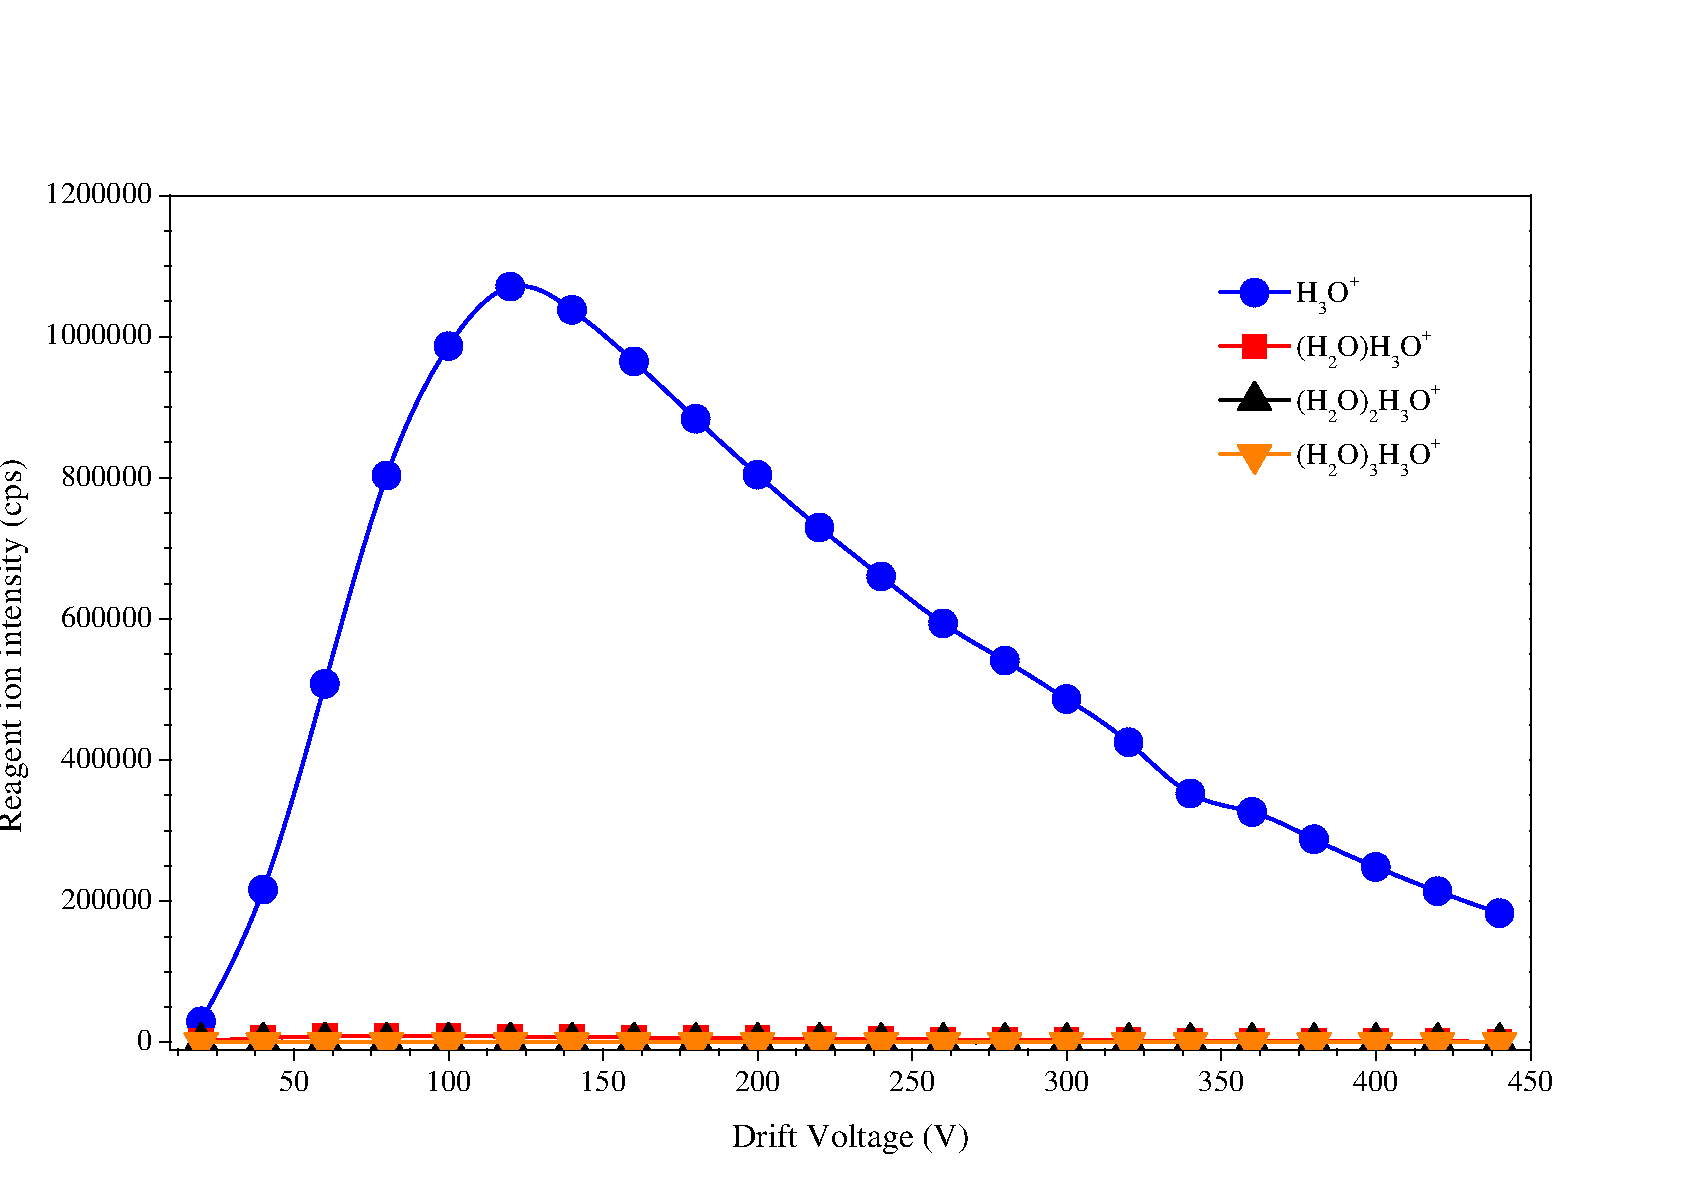
\includegraphics[width=0.8\linewidth]{pics/DPM_clusters_dry_RF.pdf}%water_RF.png}
\label{fig:ri2}}
\caption{Ion signal in counts per second (cps) for the reagent ions in (a) DC mode and (b) RF mode at 100$^{\circ}$C and 1 mbar. \textbf{Bottom one is from Lynx (MkII reactor)}}
\label{fig:ri}
\end{figure}




\section{Results and discussion}
\subsection{Measurement of illicit drugs in DC mode}

\subsubsection{Cocaine}



\begin{table}%[ht]
\centering
\caption{Proton affinity, PA, and Gibbs free energy, GB, of the main protonation sites of cocaine.}
\label{tb:co1}
\begin{tabular}{lcc}
\toprule
\textbf{Structure} &\textbf{PA (kJ/mol)} &\textbf{GB (kJ/mol)}\\ \toprule
Cocaine1H$^+$  & 1013 &   980    \\
Cocaine2H$^+$  &933 &   895    \\
\bottomrule
\end{tabular}
\end{table}

\begin{table}%[ht]
\centering
\caption[Energetics relative to cocaine and H$_3$O$^+$.]{Energetics relative to cocaine and H$_3$O$^+$ and, in brackets, to cocaine and (H$_2$O)H$_3$O$^+$. Note that m/z refers to the detected ion, i.e. where the charge remains, and that the neutral H$_2$O has been omitted in all the cases.}
\label{tb:co2}
\begin{tabular}{lccc}
\toprule
\textbf{Reaction or transition state}	&\textbf{m/z} &\textbf{$\Delta$H$_{298}$} &\textbf{$\Delta$G$_{298}$}\\
& &	\textbf{(kJ/mol)} &\textbf{(kJ/mol)} \\  \toprule
Cocaine1H$^+$  				&	304	& -328 (-170)  & -326 (-202)   \\ \midrule
(CocaineH$^+$ - MeOH) + MeOH   			&	272	& -138 (+20)	&-186 (-62)   \\ \midrule
(CocaineH - benzoic acid)$^+$ + benzoic acid &	182 & -272 (-114)  & -336 (-212)  \\ \midrule
(CocaineH - benzoyl) + benzoyl$^+$    	&	105	& -54 (+104)  & -104 (+20)  \\ \midrule
(Cocaine - benzoic acidH) + benzoic acidH$^+$& 123	& -88 (+70)  & -144  (-20) \\ \midrule
MeOH loss: TS2 for H migration O3 to O5& & -8 (+150)  & -9 (+115)  \\ \midrule
MeOH loss: TS2A for H migration O2 to O5& & -119 (+39)  & -111  (+13) \\ 
\bottomrule
\end{tabular}
\end{table}



\begin{figure}%[h]
\centering
\scalebox{0.5}{
\begin{tikzpicture}
\chemfig{[:180]**6(------)-[::210](=[::60]O^2)-[::-60]O^4>[::75](?[a])-[::30]-[::-60,1.4](<:[::60]H)(-[::-60]N^1?[b,{-}]-[::15])-[::90,1.1]-[::135,0.8]-[::45,1.1](?[b])(<[::0]H)-[::-60]?[a](<[::45](=[::60]O^3)-[::-60]O^5-[::60])}
%\chemfig{[:180]**6(------)-[::210](=[::60]O)-[::-60]O>[::75](?[a])-[::30]-[::-60,1.4](<:[::60]H)(-[::120]N?[b,{-}]-[::-15])-[::-30,1.1]-[::-90,0.8]-[::-90,1.1](?[b])(<[::105]H)-[::60]?[a](<[::45](=[::60]O)-[::-60]O-[::60])} %previous version with the N in opposite way
\end{tikzpicture}
}\label{fig:coc}
\caption{Cocaine}
\end{figure}

\begin{figure}
\begin{center}
\begin{tikzpicture}[scale=1.0]
\tikzstyle{every node}=[font=\small]
\begin{axis}[clip=false,ylabel=$\Delta$G (kJ/mol),xlabel=Reaction coordinate,xtick=\empty,
legend pos=outer north east,xmin=0.5,xmax=14,ymax=120,ymin=-220,axis lines = left]
\addplot[color=black,draw=blue,line width=1pt] coordinates {(2,0)(3,0)};
\addplot[color=black,line width=0.8pt,densely dotted] coordinates {(3,0)(4,-178)};
\addplot[color=black,draw=blue,line width=1pt] coordinates {(4,-178)(5,-178)};
\addplot[color=black,line width=0.8pt,densely dotted] coordinates {(5,-178)(6,-41)};
\addplot[color=black,draw=blue,line width=1pt] coordinates {(6,-41)(7,-41)};
\addplot[color=black,line width=0.8pt,densely dotted] coordinates {(7,-41)(8,-120)};
\addplot[color=black,draw=blue,line width=1pt] coordinates {(8,-120)(9,-120)};
\addplot[color=black,line width=0.8pt,densely dotted] coordinates {(9,-120)(10,71)};
\addplot[color=black,draw=blue,line width=1pt] coordinates {(10,71)(11,71)};
\addplot[color=black,line width=0.8pt,densely dotted] coordinates {(11,71)(12,-77)};
\addplot[color=black,draw=blue,line width=1pt] coordinates {(12,-77)(13,-77)};
\node [text width=2cm] at (axis cs:2.5,20) {EtBz + H$_3$O$^+$};
\node [text width=2cm] at (axis cs:4.5,-200) {EtBz1H$^+$};
\node [text width=3cm] at (axis cs:6.5,-20) {TS for loss of C$_2$H$_4$};
\node [text width=3cm] at (axis cs:8.5,-140) {Benzoic acid.H$^+$ + C$_2$H$_4$};
\node [text width=3cm] at (axis cs:10.5,90) {TS for loss of H$_2$O to Benzoyl$^+$};
\node [text width=3cm] at (axis cs:12.5,-97) {Benzoyl$^+$ + C$_2$H$_4$};
%\node at (2.5,3) {\includegraphics[scale=0.1]{rea1.pdf}};
%\node at (axis cs:2.1,-10) {\includegraphics[scale=0.06,angle=90]{r1.pdf}};
%\node at (axis cs:3.2,-10) {\includegraphics[scale=0.06,angle=90]{r2.pdf}};
%\node at (axis cs:4.3,50) {\includegraphics[scale=0.08,angle=90]{t1.pdf}};
%\node at (axis cs:6.9,-35) {\includegraphics[scale=0.08,angle=90]{p1.pdf}};
\end{axis}
\end{tikzpicture}
\end{center}
\caption{$\Delta$G for reaction of H$_3$O$^+$ with EtBz –- Example of the data from Peter Watts}\label{fig:trans.example}
\end{figure}

\newpage

\begin{table}%[ht]
\centering
\caption[Energetics relative to ethyl benzoate and H$_3$O$^+$.]{Energetics relative to ethyl benzoate and H$_3$O$^+$. Note that m/z refers to the detected ion, i.e. where the charge remains, and that the neutral H$_2$O has been omitted in all the cases.}
\label{tb:eb2}
\begin{tabular}{lccc}
\toprule
\textbf{Reaction or transition state}	&\textbf{m/z} &\textbf{$\Delta$H$_{298}$} &\textbf{$\Delta$G$_{298}$}\\
& &	\textbf{(kJ/mol)} &\textbf{(kJ/mol)} \\  \toprule
EtBz1H$^+$   					&	151	& -180  & -178   \\ \midrule
EtBz2H$^+$   					&	151	& -95  & -97   \\ \midrule
Benzoyl$^+$  + EtOH				&	105	& -36  & -83   \\ \midrule
TS to above, i.e. to 2H$^+$		&		& -3  & +2   \\ \midrule
Benzoic acid.H$^+$ + C$_2$H$_4$	&	123	& -74  & -120   \\ \midrule
TS1 for loss of ethene from 1H$^+$	&		& -36  & -41   \\ \midrule
TS2 for loss of ethene from 2H$^+$	&		& -15  & -14   \\ \midrule
Benzoyl$^+$  + C$_2$H$_4$ + H$_2$O	&	105	& +15  & -77   \\ \midrule
%\multicolumn{2}{l}{TS3 to above(loss of H$_2$O from benzoic acid.H$^+$)}		& +98  & +52   \\ \midrule
TS3 to above, i.e.	&		&   &    \\ 
loss of H$_2$O from benzoic acid.H$^+$	&		& +98  & +52   \\ \midrule
Benzene.H$^+$	+ C$_2$H$_4$ + H$_2$O &	79	& +34  & -132   \\ 
\bottomrule
\end{tabular}
\end{table}


\begin{figure}%[h]
\begin{center}
\schemedebug{false}
\schemestart[0,1,thick]
\chemname{\scalebox{0.4}{\chemfig{**6(----(-[::-60](=[::60]O^1)-[::-60]O^2(-[::60]-[::-60]))--)}
}\+\chemfig{H_3O^+}}{Ethyl benzoate}
\arrow(nph.south--aa7)[-150,2]
		\chemname{\scalebox{0.4}{\chemfig{**6(----(-[::-60](-[,0.2,,,draw=none]\+)(-[::60]O-[::-60]H)-[::-60]O(-[::60]-[::-60]))--)}
}}{Ethyl benzoate 1H$^+$}
	\arrow[-90]
		\chemname{\scalebox{0.4}{\chemfig{**6(----(-[::-60](-[,0.2,,,draw=none]\+)(-[::60]O-[::-60]H)-[::-60]O(-[@{db}::-30]-[@{a1}::90]-[@{db2}::90]H-[@{a2}::90,,,,draw=none]))--)}
    	\chemmove{\draw(db)..controls +(120:4mm) and +(150:4mm)..(a1);
    	\draw(db2)..controls +(-60:4mm) and +(-30:4mm)..(a2);}}%\+\chemfig{H_2O}
                }{TS1 from 1H$^+$}
	\arrow(aa11--ba)[-90]
    	\chemname{\scalebox{0.4}{\chemfig{**6(----(-[::-60](-[,0.2,,,draw=none]\+)(-[::60]O-[::-60]H)-[::-60]O(-[::60]H))--)}
}}{Benzoic acid.H$^+$}
	\arrow(@ba--)[-90]
    	\chemname{\scalebox{0.4}{\chemfig{**6(----(-[::-60](-[,0.2,,,draw=none]\+)(-[@{a3}::60]O-[@{db3}::-60]H-[@{a4}::-120,1.5,,,draw=none])-[@{db4}::-60]O(-[::60]H))--)}
        \chemmove{\draw(db3)..controls +(0:4mm) and +(90:4mm)..(a3);
    	\draw(db4)..controls +(270:4mm) and +(270:4mm)..(a4);}
        }}{TS3 (loss of water)}
	\arrow(aa10--aa2)[0,3.7]
    	\chemname{\scalebox{0.4}{\chemfig{**6(----(-[::-60](-[,0.2,,,draw=none]\+)=[::60]O)--)}}}{Benzoyl$^+$}
\arrow(@nph.south--aa3)[-30,2]
		\chemname{\scalebox{0.4}{\chemfig{**6(----(-[::-60](=[::60]O)-[::-60]O^+(-[::-60]H)(-[::60]-[::-60]))--)}
}}{Ethyl benzoate 2H$^+$}
	\arrow(.south--aa4)[-135,2.5]
    	\chemname{\scalebox{0.4}{\chemfig{**6(----(-[::-60](*6(-O^+(-[::-60]H)-[@{db6}]-[@{a6}]-H-[@{a5},,,,draw=none]O=[@{db5}])))--)}
		\chemmove{\draw(db5)..controls +(60:4mm) and +(0:4mm)..(a5);
    	\draw(db6)..controls +(180:4mm) and +(240:4mm)..(a6);}
		}}{TS2 from 2H$^+$}
     \arrow(@aa3.south--@aa2)
    \arrow(@aa4.mid west--@ba)
    \arrow(@aa7--aa8.)[0,1.3]
        	\chemname{\scalebox{0.4}{\chemfig{**6(----(-[::-60](*6(-O^+(-[@{db6}::-60,,,,draw=none])-(-[::-60])-[,,,,draw=none]-[,,,,draw=none]H(-[@{a6}::-240,,,,draw=none])-[@{a5}]O-[@{db5}])))--)}
		\chemmove{\draw(a5)..controls +(0:4mm) and +(60:4mm)..(db5);
		\draw(db6)..controls +(-120:10mm) and +(-90:10mm)..(a6);}
		}}{TS from 1H$^+$ to 2H$^+$}
		\arrow(.east--aa3)[0,1.3]
\schemestop
\end{center}
\caption{Ethyl benzoate}\label{fig:eb1}
\end{figure}





\subsubsection{Ecstasy}

\begin{figure}%[h]
\centering
\scalebox{0.5}{
\chemfig{*6(=-*5(-O--O-?[a]=)--=(--[::60](-[::60])-[::-60]N(-[::-60]H)-[::60])-)}}
\caption{MDMA}\label{fig:mdma}
\end{figure}



\subsubsection{Codeine}

\begin{figure}%[h]
\centering
\scalebox{0.5}{
\chemfig{[:-120]**6(-(-O@{a1}-[::300])-?[a]-*6(-(<[::130,1]-[::-45,1.5,,,line width=3pt]?[b])*6(-(<:[::-80,1.25]O?[a])(<[::0]H)-(<:O-[::60]H)-=-)-(<[::-30]H)-(<:[::-105]H)(-N?[b,{>}]-[::-30])--)---)}}
\caption{codeine}\label{fig:cod}
\end{figure}



\subsubsection{Morphine}


\begin{figure}%[h]
\centering
\scalebox{0.5}{
\begin{tikzpicture}\chemfig{[:-120]**6(-(-O-[::-60]H)-?[a]-*6(-(<[::130,1]-[::-45,1.5,,,line width=3pt]?[b])*6(-(<:[::-80,1.25]O?[a])(<[::0]H)-(<:O-[::60]H)-=-)-(<[::-30]H)-(<:[::-105]H)(-N?[b,{>}]-[::-30])--)---)}
\end{tikzpicture}}
\caption{morphine}\label{fig:mor}
\end{figure}



\subsubsection{Heroin}

\begin{figure}%[h]
\centering
\scalebox{0.5}{
\begin{tikzpicture}
\chemfig{[:-120]**6(-(-O@{a1}-[::300](=[@{db}::-60]O)-[::60])-?[a]-*6(-(<[::130,1]-[::-45,1.5,,,line width=3pt]?[b])*6(-(<:[::-80,1.25]O?[a])(<[::0]H)-(<:\chemabove{O}{\scriptstyle\oplus}-[::60](-[::-60])=[::60]O)-=-)-(<[::-30]H)-(<:[::-105]H)(-N?[b,{>}]-[::-30])--)---)}
\end{tikzpicture}}
\caption{Heroin}\label{fig:her}
\end{figure}


\subsubsection{Cocaine-related compounds}

\begin{figure}%[h]
\begin{center}
\begin{subfloatrow}
\sidesubfloat[]{\scalebox{0.5}{
\chemfig{**6(------)-[::210](=[::60]O)-[::-60]O(-[::60]H-[::-60,,,,white])}}\label{fig:ba}}
\quad\quad
\sidesubfloat[]{\scalebox{0.5}{
\chemfig{**6(------)-[::210](=[::60]O)-[::-60]O(-[::60]-[::-60,,,,white])}}\label{fig:mb2}}
\quad\quad
\sidesubfloat[]{\scalebox{0.5}{
\chemfig{**6(------)-[::210](=[::60]O)-[::-60]O(-[::60]-[::-60])}}\label{fig:eb}}
\end{subfloatrow}
\bigskip
%\begin{subfloatrow}
\sidesubfloat[]{\scalebox{0.5}{
\chemfig{**6(------)-[::210](=[::60]O)-[::-60]O(-[::60](-[::60])-[::-60])}}\label{fig:ib}}
\quad\quad
\sidesubfloat[]{\scalebox{0.5}{
\chemfig{**6(------)-[::210](=[::60]O)-[::-60]O-[::60](=[::60]O)-[::-60]**6(------)}}\label{fig:ban}}
%\end{subfloatrow}
\end{center}
\caption{Structure of (a) benzoic acid,  (b) methyl benzoate, (c) ethyl benzoate, (d) isopropyl benzoate and (e) benzoic anhydride.}\label{fig:cocr}
\end{figure}




\begin{table}%[ht]
\centering
\caption{Proton affinity, PA, and Gibbs free energy, GB, of the main protonation sites of methyl benzoate.}
\label{tb:mb1}
\begin{tabular}{lcc}
\toprule
\textbf{Structure} &\textbf{PA (kJ/mol)} &\textbf{GB (kJ/mol)}\\ \toprule
MeBz1H$^+$  & 839 &   808    \\
MeBz2H$^+$  & 764 &   741    \\
\bottomrule
\end{tabular}
\end{table}

\begin{table}%[ht]
\centering
\caption[Energetics relative to methyl benzoate and H$_3$O$^+$.]{Energetics relative to methyl benzoate and H$_3$O$^+$. Note that m/z refers to the detected ion, i.e. where the charge remains, and that the neutral H$_2$O has been omitted in all the cases.}
\label{tb:mb2}
\begin{tabular}{lccc}
\toprule
\textbf{Reaction or transition state}	&\textbf{m/z} &\textbf{$\Delta$H$_{298}$} &\textbf{$\Delta$G$_{298}$}\\
& &	\textbf{(kJ/mol)} &\textbf{(kJ/mol)} \\  \toprule
MeBz1H$^+$   					&	137	& -155  & -155   \\ \midrule
Benzoyl$^+$ + MeOH				&	105	& -29  & -82   \\ \midrule
TS to above, i.e. to 2H$^+$\footnote[2]{I don't get this}&		& +15  	& +14\\ \midrule
MeBz2H$^+$ 						&	137	& -80  & -88   \\ 
\bottomrule
\end{tabular}
\end{table}

\begin{figure}%[h]
\begin{center}
\scalebox{0.5}{
\chemfig{**6(----(-[::-60](=[::60]O^1)-[::-60]O^2(-[::60]))--)}
}
\end{center}
\caption{Methyl benzoate}
\end{figure}


\begin{figure}%[h]
\centering
\scalebox{0.5}{
\begin{tikzpicture}
\chemfig{[:180]**6(------)-[::210](=[::60]O^2)-[::-60]O^4>[::75](?[a])-[::30]-[::-60,1.4](<:[::60]H)(-[::-60]N^1?[b,{-}]-[::15])-[::90,1.1]-[::135,0.8]-[::45,1.1](?[b])(<[::0]H)-[::-60]?[a](<[::45](=[::60]O^3)-[::-60]O^5-[::60]H)}
\end{tikzpicture}}
\caption{Benzoyl ecgonine}\label{fig:be}
\end{figure}


\begin{figure}%[h]
\centering
\scalebox{0.5}{
\begin{tikzpicture}
\chemfig{[:180]**6(------)-[::210](=[::60]O^2)-[::-60]O^4>[::75](?[a])-[::30]-[::-60,1.4](<:[::60]H)(-[::-60]N^1?[b,{-}]-[::15])-[::90,1.1]-[::135,0.8]-[::45,1.1](?[b])(<[::0]H)-[::-60]?[a](<[::45](=[::60]O^3)-[::-60]O^5-[::60]-[::-60])}
%\chemfig{[:180]**6(------)-[::210](=[::60]O)-[::-60]O>[::75](?[a])-[::30]-[::-60,1.4](<:[::60]H)(-[::120]N?[b,{-}]-[::-15])-[::-30,1.1]-[::-90,0.8]-[::-90,1.1](?[b])(<[::105]H)-[::60]?[a](<[::45](=[::60]O)-[::-60]O-[::60])} %previous version with the N in opposite way
\end{tikzpicture}
}\label{fig:cocet}
\caption{Cocaethylene}
\end{figure}




\begin{table}%[ht]
\centering
\caption{Proton affinity, PA, and Gibbs free energy, GB, of the main protonation sites of methyl ecgonine.}
\label{tb:me1}
\begin{tabular}{lcc}
\toprule
\textbf{Structure} &\textbf{PA (kJ/mol)} &\textbf{GB (kJ/mol)}\\ \toprule
MeEcg1H$^+$  & 996 &   965    \\
MeEcg3H$^+$  & 906 &   873    \\
\bottomrule
\end{tabular}
\end{table}

\begin{table}%[ht]
\centering
\caption[Energetics relative to methyl ecgonine and H$_3$O$^+$.]{Energetics relative to methyl ecgonine and H$_3$O$^+$. Note that m/z refers to the detected ion, i.e. where the charge remains, and that the neutral H$_2$O has been omitted in all the cases.}
\label{tb:me2}
\begin{tabular}{lccc}
\toprule
\textbf{Reaction or transition state}	&\textbf{m/z} &\textbf{$\Delta$H$_{298}$} &\textbf{$\Delta$G$_{298}$}\\
& &	\textbf{(kJ/mol)} &\textbf{(kJ/mol)} \\  \toprule
MeEcg1H$^+$   				&	200	& -312  & -312   \\ \midrule
(MeEcgH - MeOH)$^+$ + MeOH	&	168	& -118  & -171   \\ \midrule
TS for loss of MeOH			&		& +4  	& 0   		\\ \midrule
(MeEcgH - H$_2$O)$^+$ + H$_2$O	&	182	& -260  & -320   \\ 
\bottomrule
\end{tabular}
\end{table}

\begin{figure}%[h]
\centering
\scalebox{0.5}{
\begin{tikzpicture}
\chemfig{[:-30]O^4(-[::180]H)>[::60](?[a])-[::45]-[::-60,1.4](<:[::60]H)(-[::-60]N^1?[b,{-}]-[::15])-[::90,1.1]-[::135,0.8]-[::45,1.1](?[b])(<[::0]H)-[::-60]?[a](<[::45](=[::60]O^3)-[::-60]O^5-[::60])}
\end{tikzpicture}}
\caption{Methyl ecgonine}\label{fig:me}
\end{figure}



\begin{figure}%[h]
\centering
\scalebox{0.5}{
\begin{tikzpicture}
\chemfig{[:30](?[a])-[::45]-[::-60,1.4](<:[::60]H)(-[::-60]N?[b,{-}]-[::15])-[::90,1.1]-[::135,0.8]-[::45,1.1](?[b])(<[::0]H)-[::-60]?[a,{=}](<[::45](=[::60]O)-[::-60]O-[::60])}
\end{tikzpicture}}
\caption{Methyl ecgonidine}\label{fig:med}
\end{figure}



\begin{figure}%[h]
\centering
\vspace{1cm}
\sidesubfloat[]{\scalebox{0.6}{\chemfig{[:30]-[::-60]-[::60]O-[::-60]-[::60]-[::-60]O-[::60]-[::-60]-[::60]O-[::-60]-[::60]}}}\label{fig:dgde1}
\quad
\sidesubfloat[]{\scalebox{0.6}{\chemfig{[:30]-[::-60]O-[::60]-[::-60]-[::60]O-[::-60]-[::60]-[::-60]O-[::60]}}}\label{fig:dgde2}
\vspace{1cm}
\caption{Structure of (a) diethylene glycol diethyl ether and (b) diethylene glycol dimethyl ether}\label{fig:dgde}
\end{figure}

























\subsection{Measurement of illicit drugs in RF mode}


\subsection{Nitroanilines}

\begin{figure}
\vspace{0.5cm}
  \sidesubfloat[]{\scalebox{0.7}{\begin{tikzpicture}\chemfig{**6(---(-[::-60]N(-[::60]H)-[::-60]H)-(-[::-60]N^{+}(=[::60]O)-[::-60]O^{-})--)}\end{tikzpicture}}\label{fig:nit1}}
\qquad
  \sidesubfloat[]{\scalebox{0.7}{\begin{tikzpicture}\chemfig{
**6(--(-[::-60]N(-[::60]H)-[::-60]H)--(-[::-60]N^{+}(=[::60]O)-[::-60]O^{-})--)}\end{tikzpicture}}\label{fig:nit2}}
\qquad
  \sidesubfloat[]{\scalebox{0.7}{\begin{tikzpicture}\chemfig{
**6(-(-[::-60]N(-[::60]H)-[::-60]H)---(-[::-60]N^{+}(=[::60]O)-[::-60]O^{-})--)}\end{tikzpicture}}\label{fig:nit3}}
  \caption{Structure of (a) 2-nitroaniline, (b) 3-nitroaniline and (c) 4-nitroaniline.}\label{fig:nit}
\end{figure}


\begin{figure}%[h]
\centering
\sidesubfloat[]{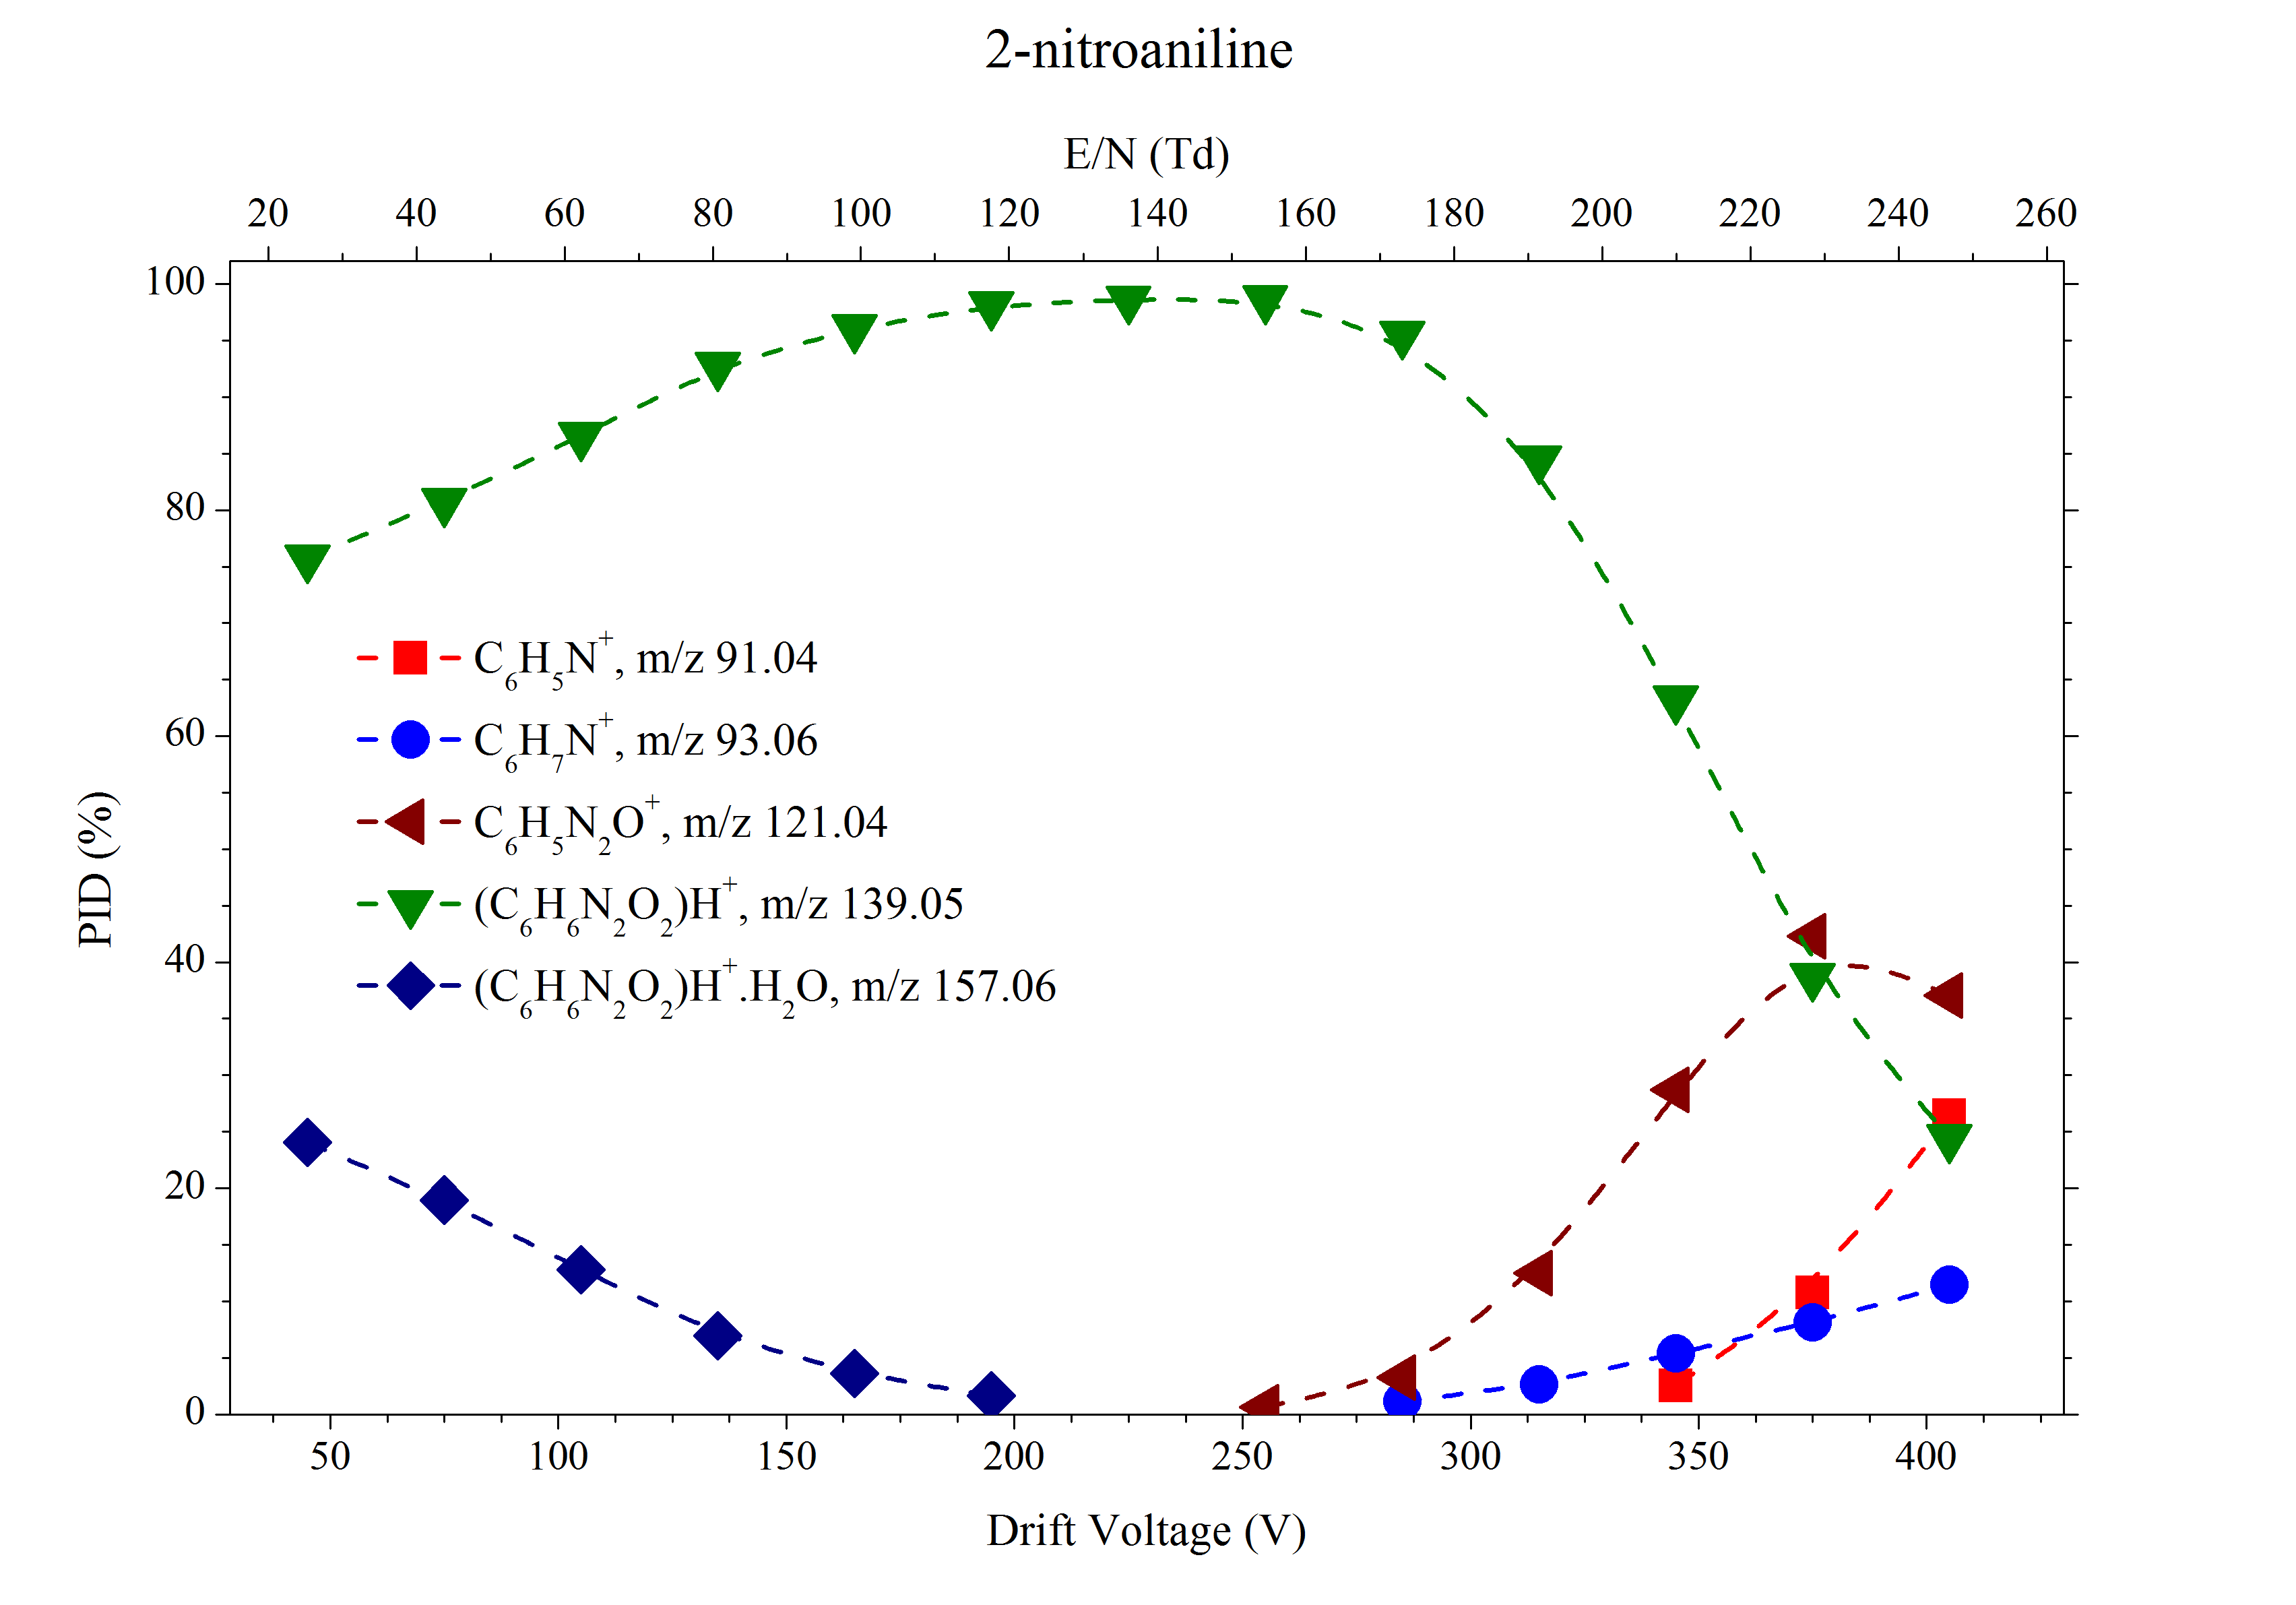
\includegraphics[width=0.6\linewidth]{pics/2-NA-h3o_DC.png}}

\sidesubfloat[]{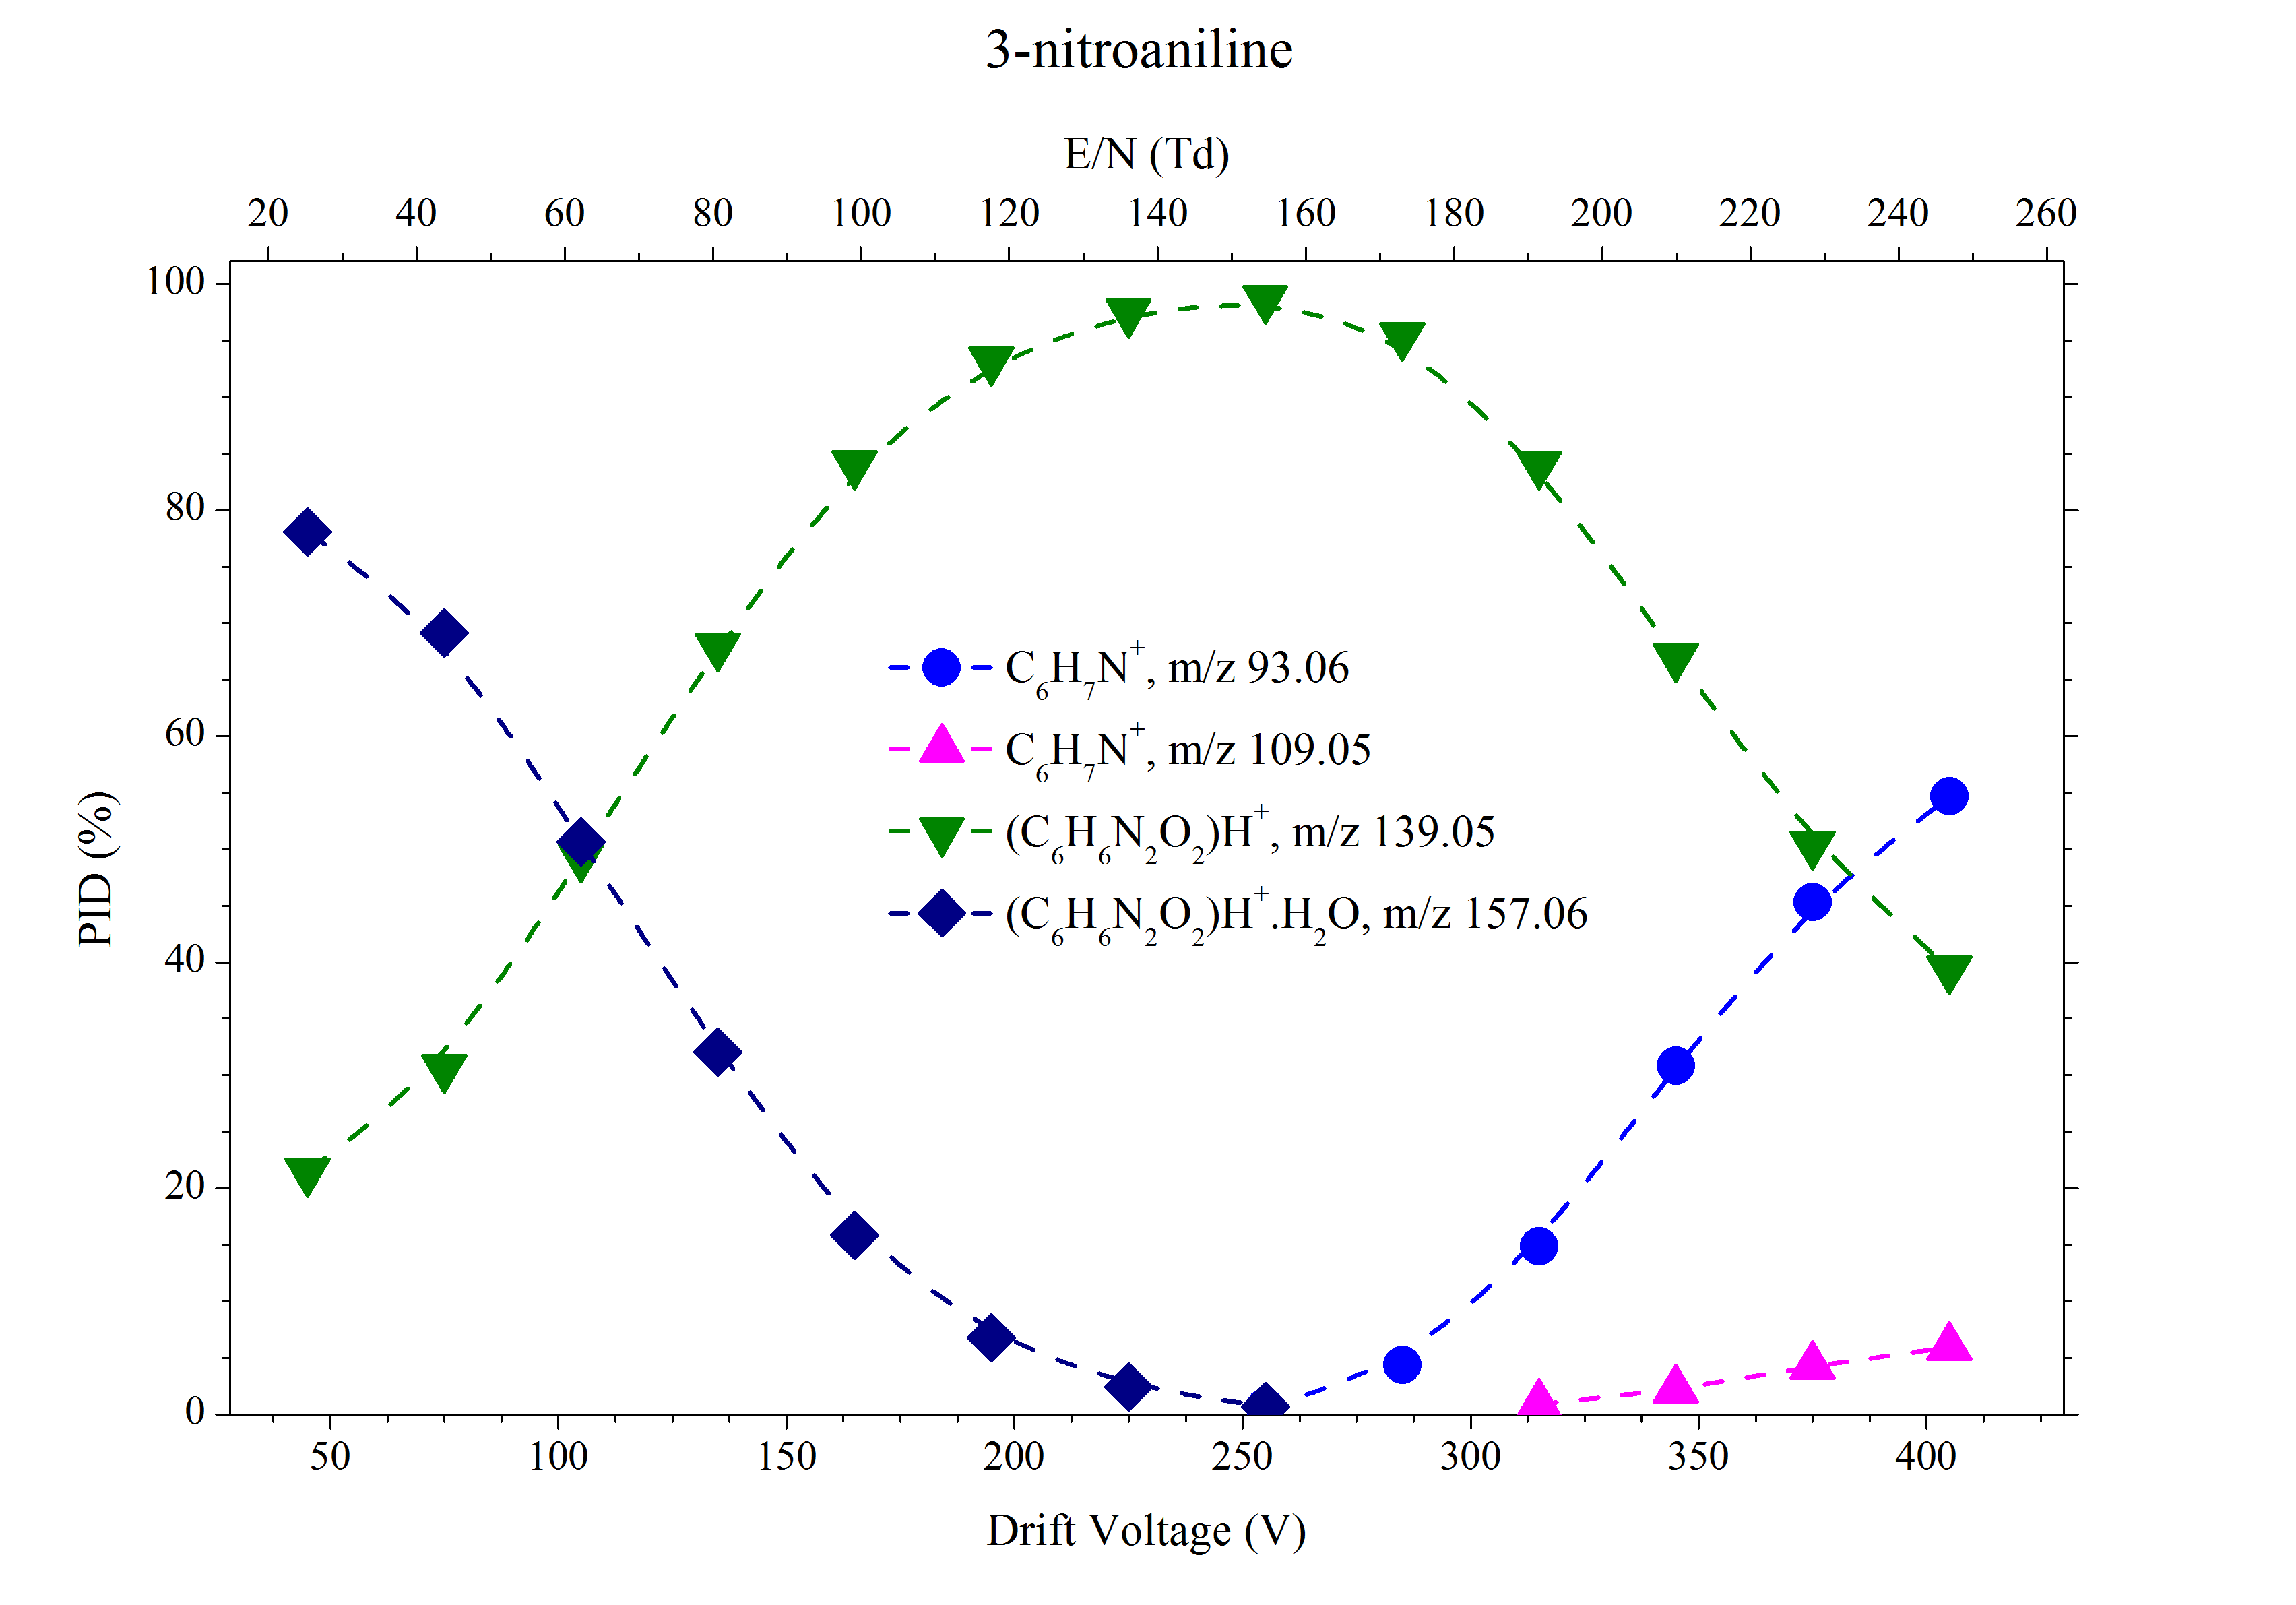
\includegraphics[width=0.6\linewidth]{pics/3-NA-h3o_DC.png}}

\sidesubfloat[]{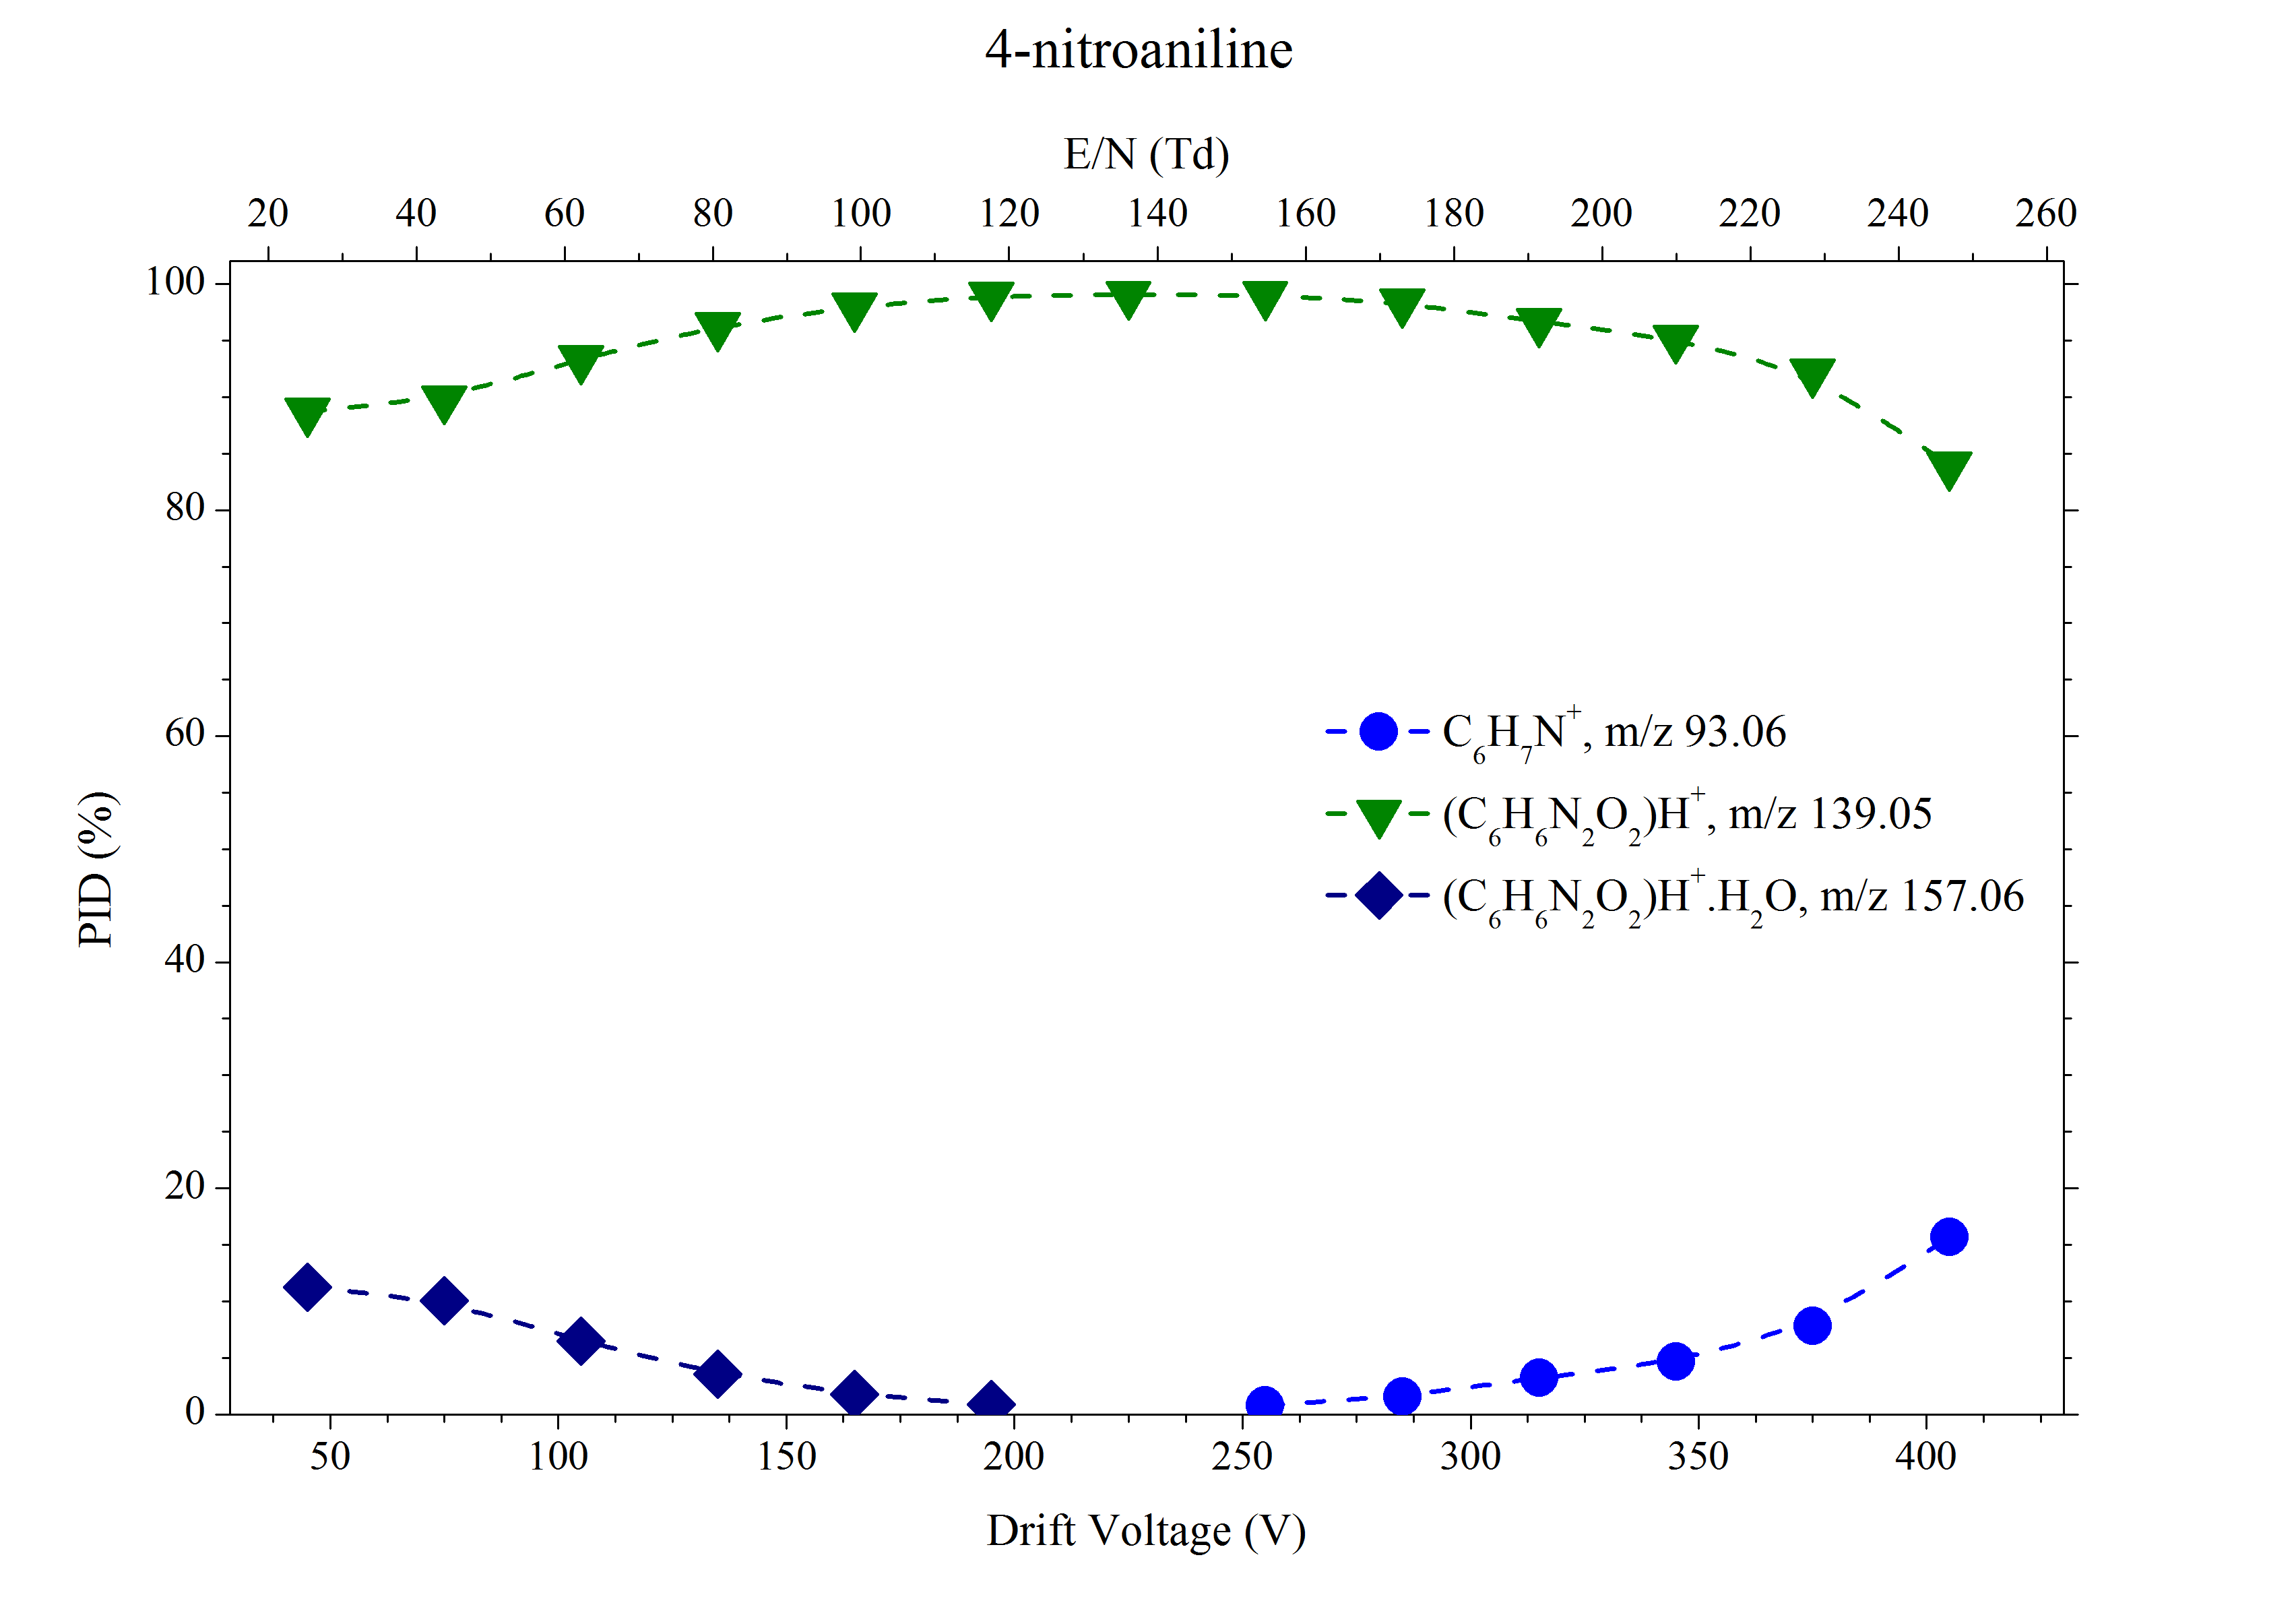
\includegraphics[width=0.6\linewidth]{pics/4-NA-h3o_DC.png}}
\caption{PID plots of (a) 2-nitroaniline, (b) 3-nitroaniline and (c) 4-nitroaniline, H3O+, DC mode}
\label{fig:na_h3o_dc}
\end{figure}

\begin{figure}%[h]
\centering
\sidesubfloat[]{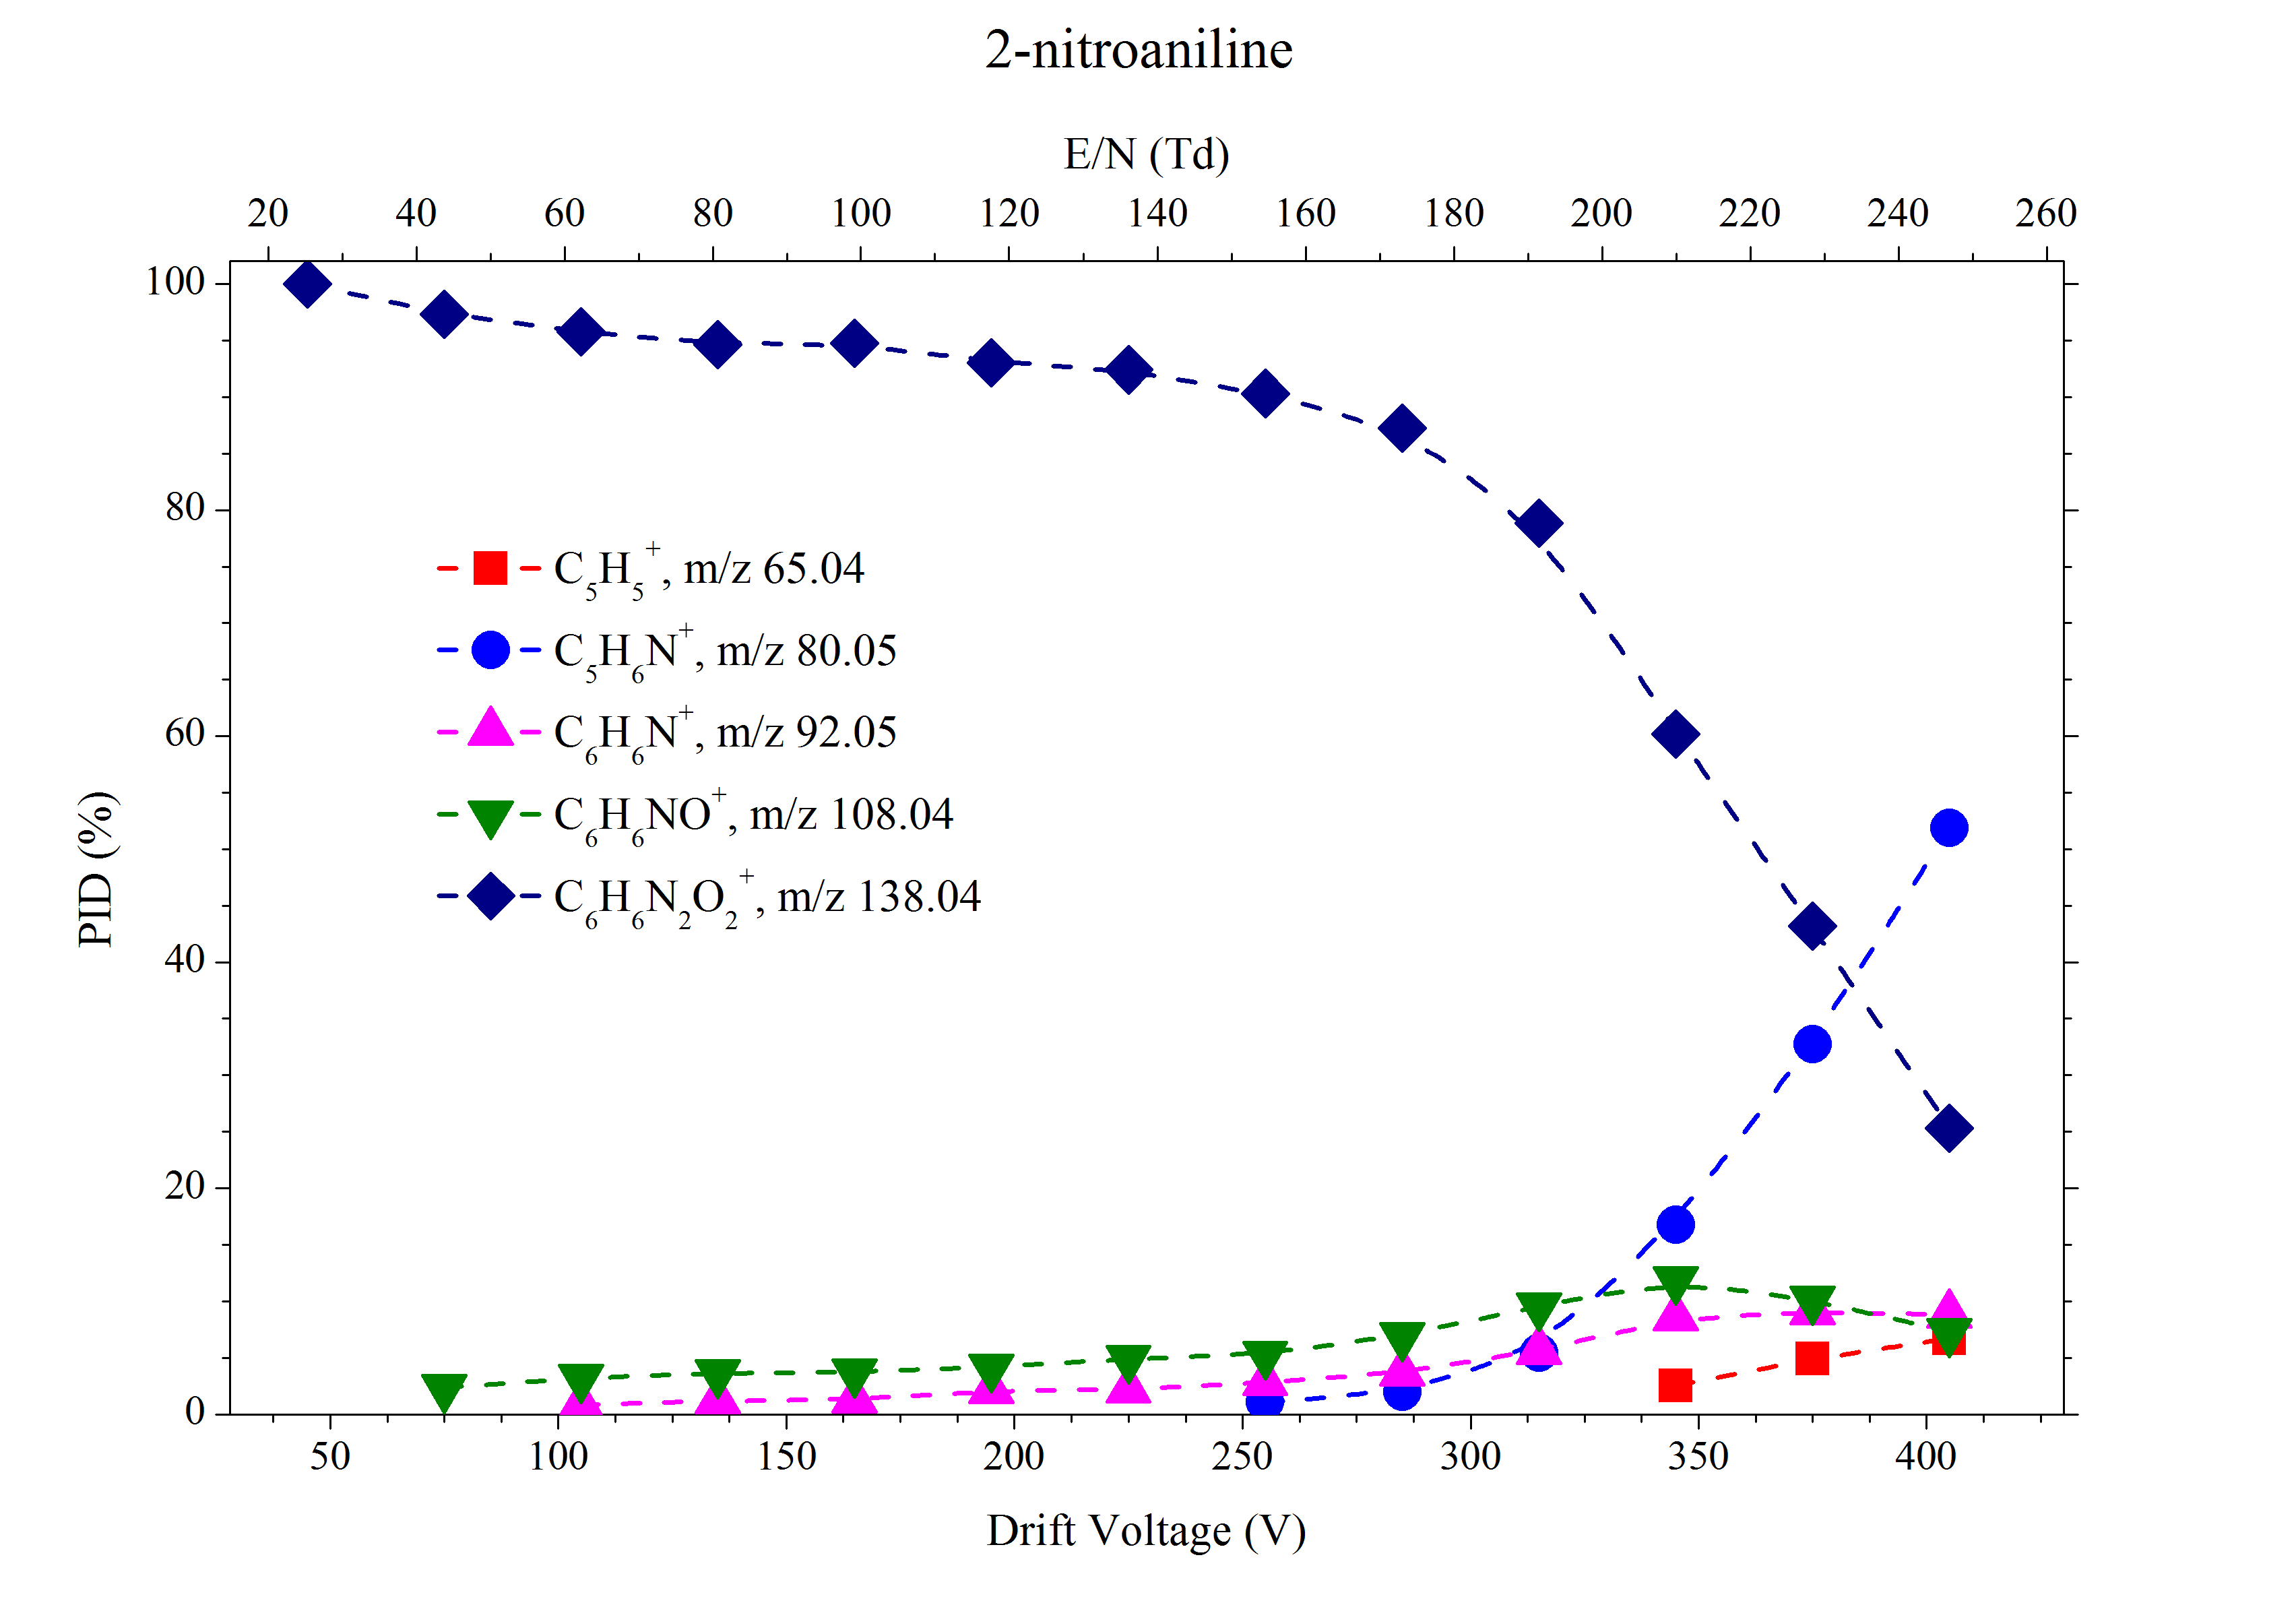
\includegraphics[width=0.6\linewidth]{pics/2-NA-o2_DC.png}}

\sidesubfloat[]{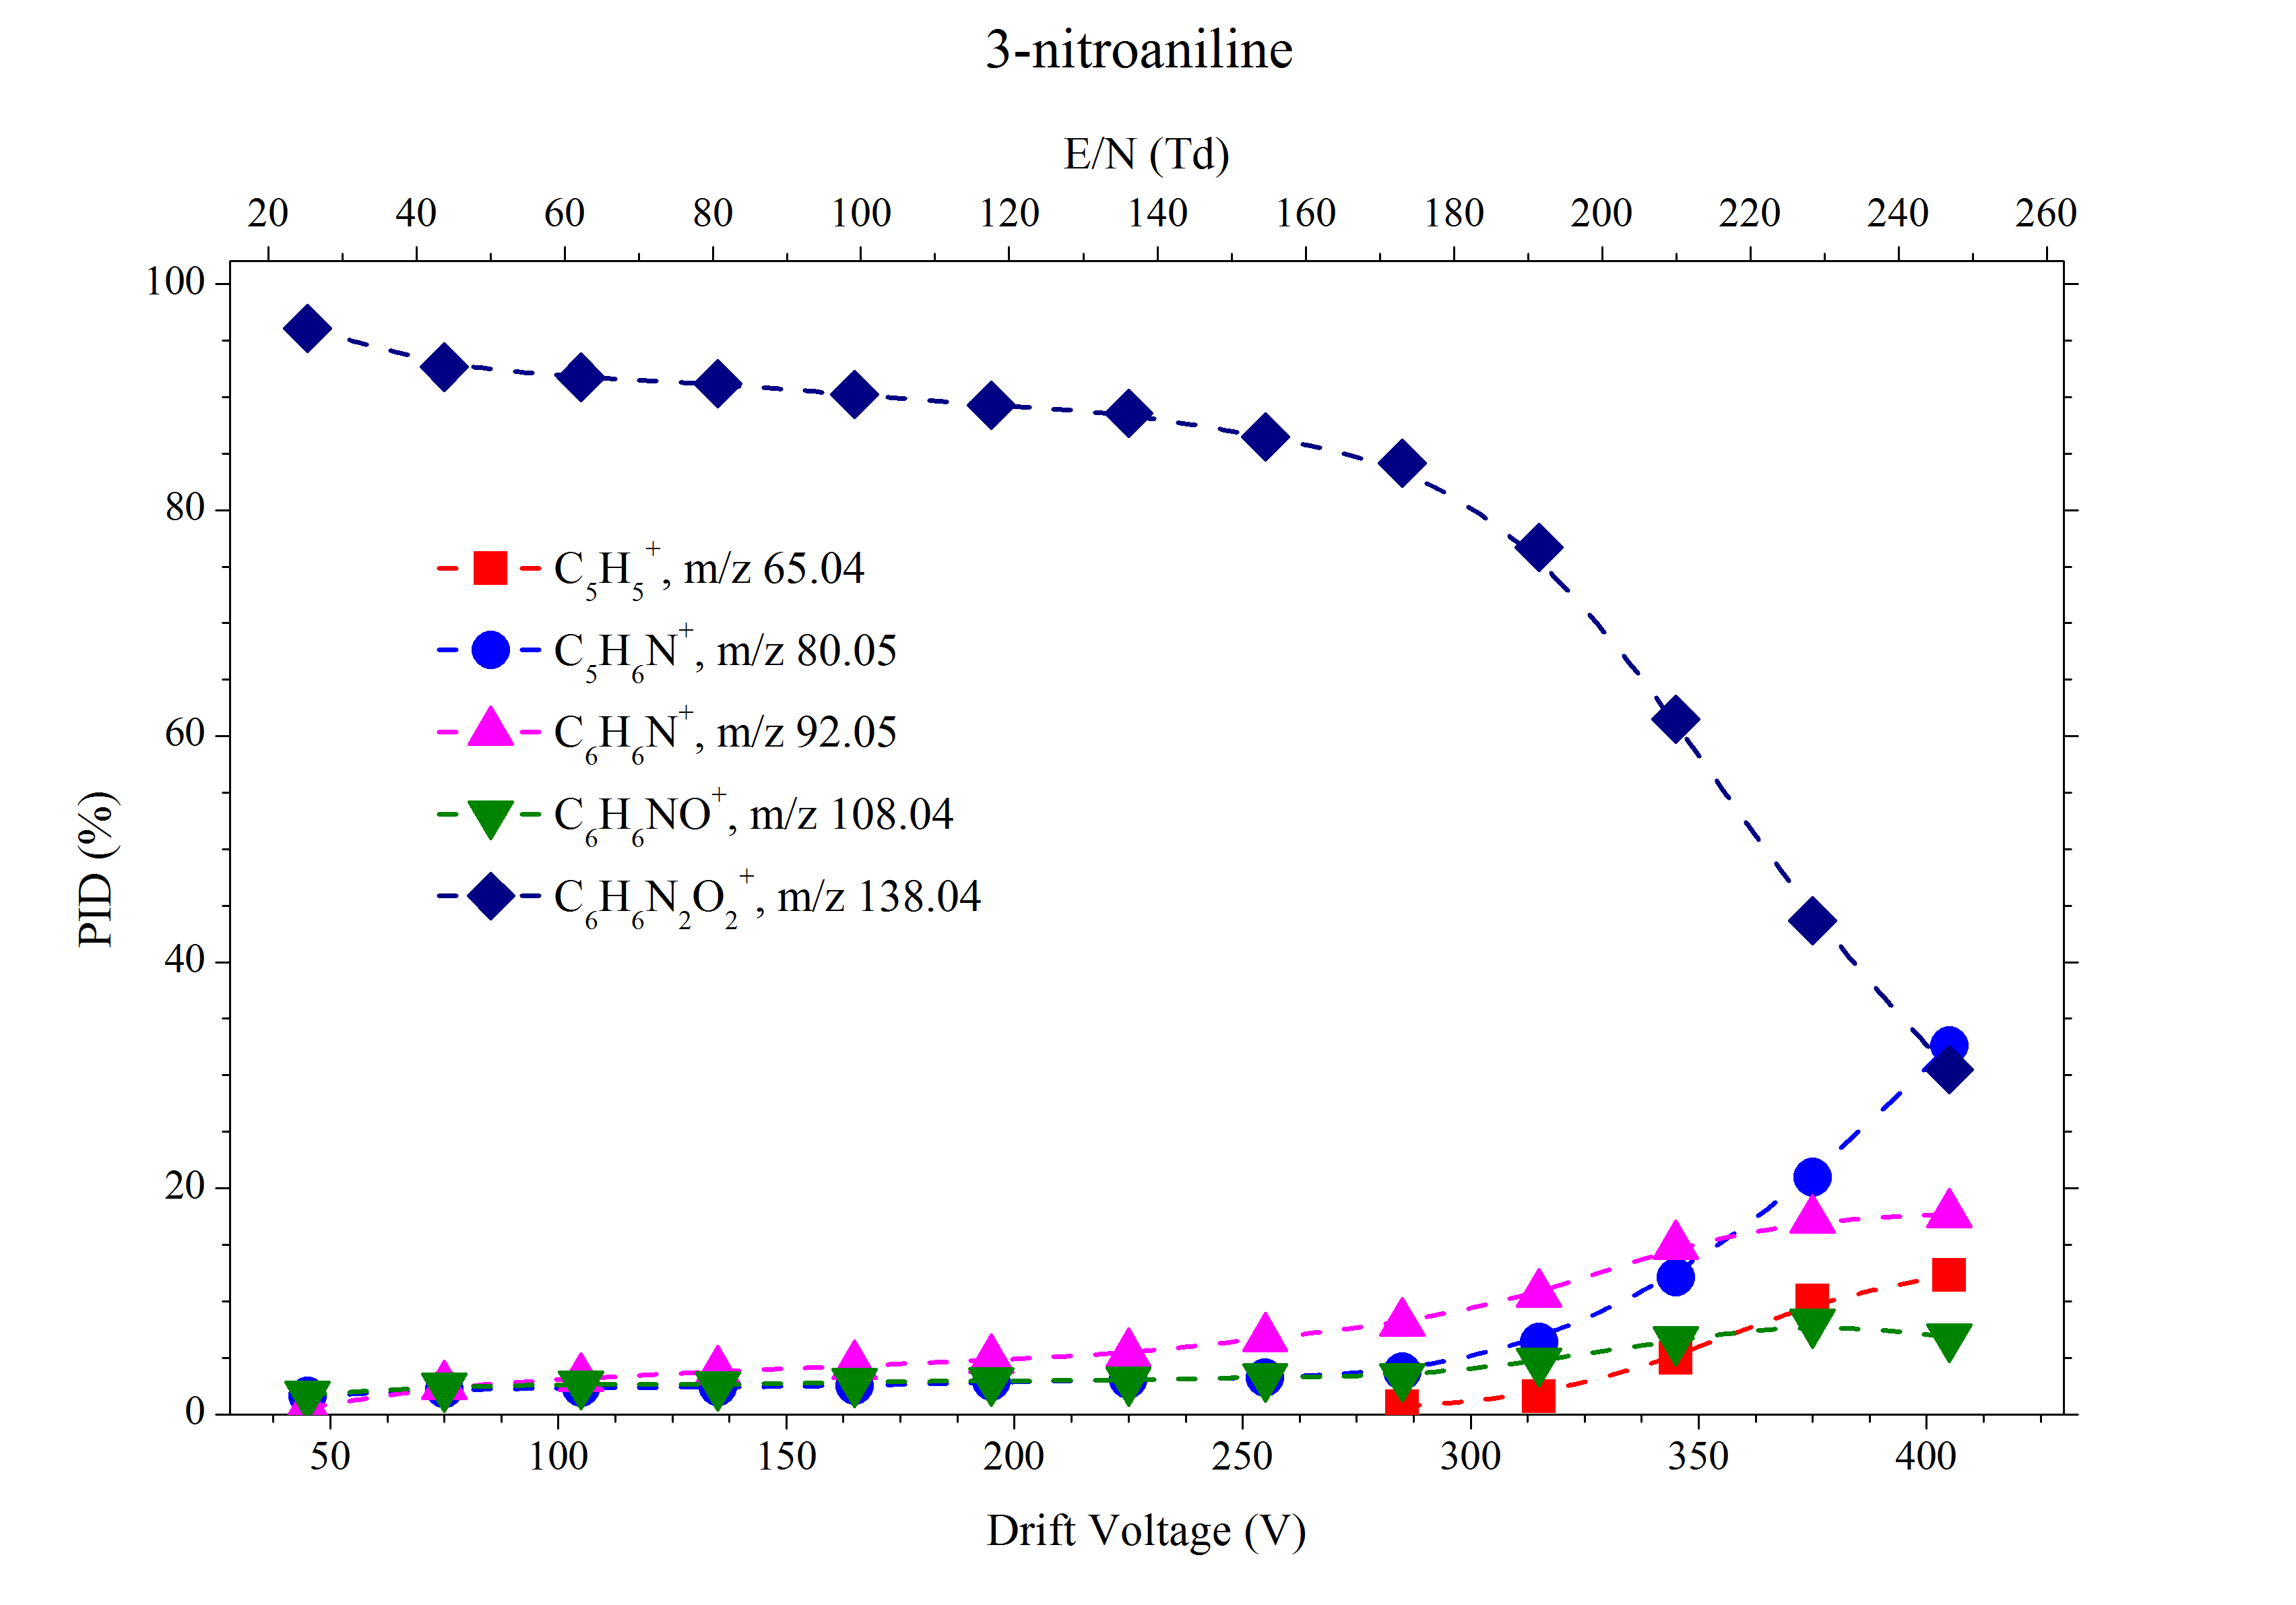
\includegraphics[width=0.6\linewidth]{pics/3-NA-o2_DC.png}}

\sidesubfloat[]{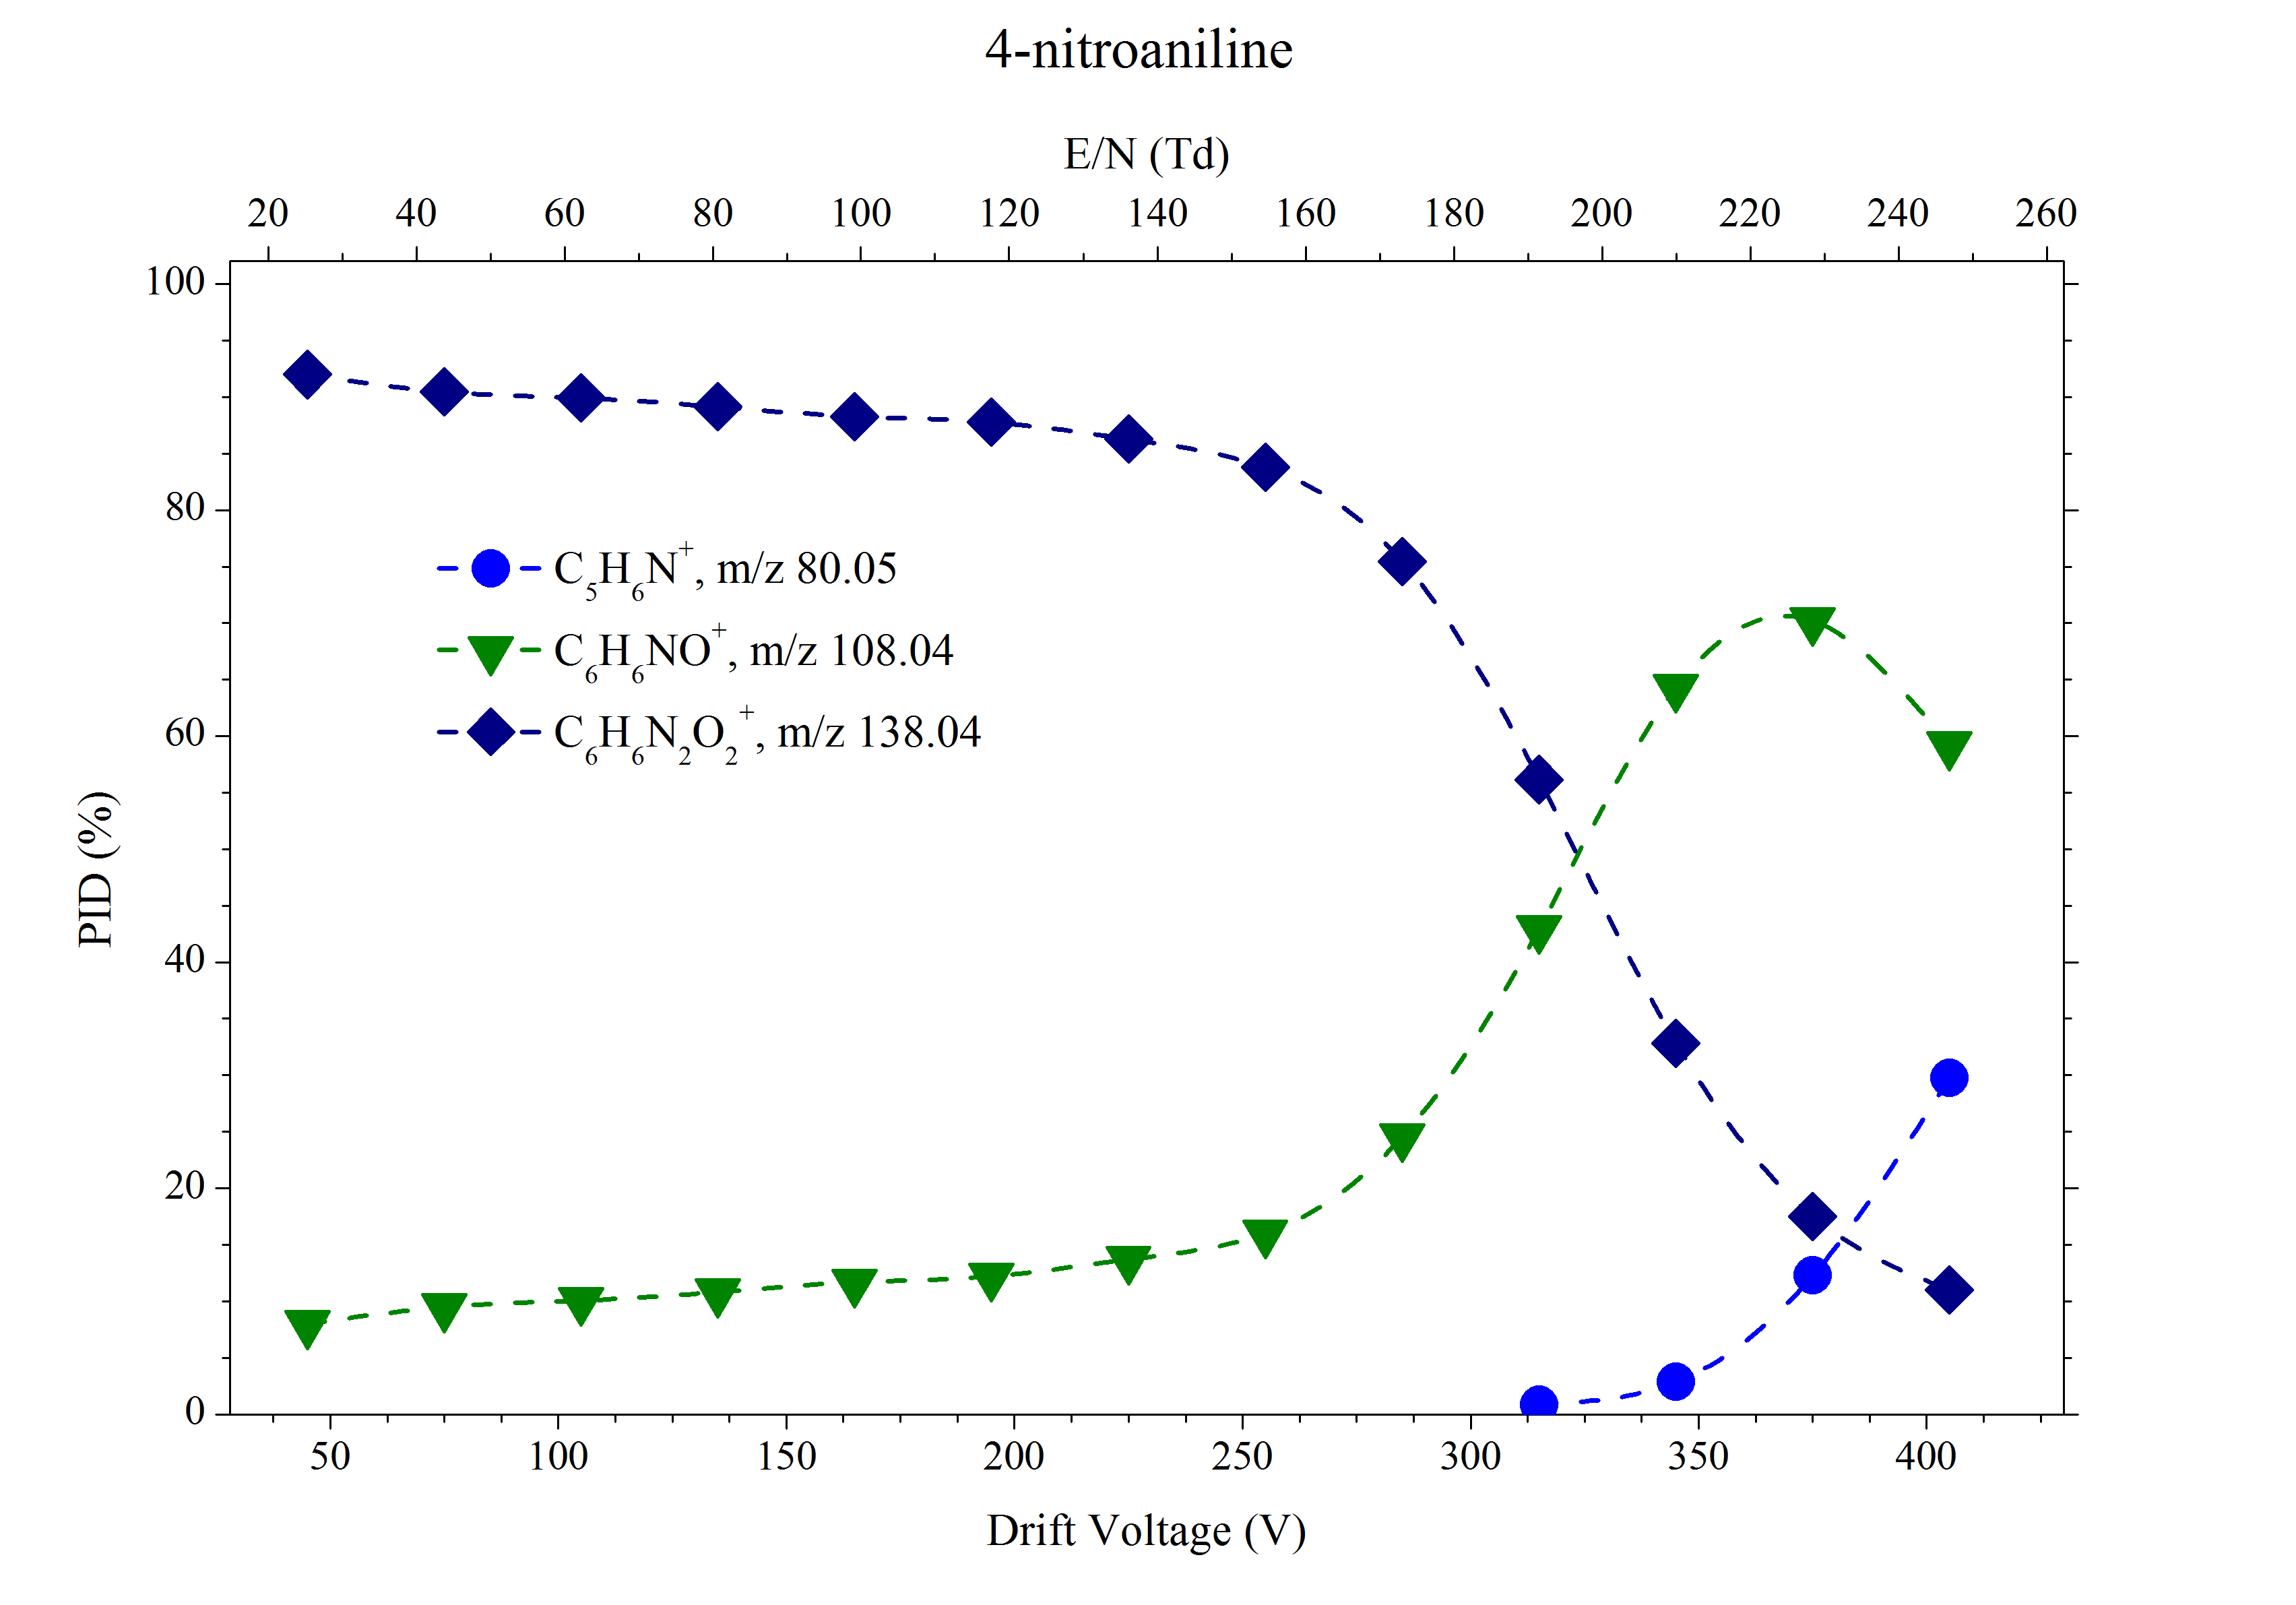
\includegraphics[width=0.6\linewidth]{pics/4-NA-o2_DC.png}}
\caption{PID plots of (a) 2-nitroaniline, (b) 3-nitroaniline and (c) 4-nitroaniline, O2+, DC mode}
\label{fig:na_o2_dc}
\end{figure}




\subsection{Characterisation of the TDU: temperature study}

\subsubsection{HMTD}
Using ------------------- as probe I have done a temperature study of the TDU keeping the rest of the temperatures and pressures constant.

Use HMTD for this (I can't put this in my thesis as it is in a paper already. put reference to the paper)   

\textbf{use the counts per second!!! It is what makes sense}

I measured at different TDU temperatures: 100$^{\circ}$C, 150$^{\circ}$C and 200$^{\circ}$C, while keeping the inlet line and the oven at 150$^{\circ}$C, so the differences come purely from the TDU temperature


\begin{figure}
\scalebox{0.7}{\begin{tikzpicture}\chemfig{N(-[::90,,,,line width=3pt]>[::-30]O-[::-30]O-[::-45]-[::-75]N?[b])(-[::-30,,,,line width=3pt]>[::30]O-[::30]O-[::30]?[b])(-[::-150,,,,line width=3pt]>[::-135]O-[::-45]O-[::-30]?[b])
}\end{tikzpicture}}
\caption{Structure of HMTD.}\label{fig:hmtd}
\end{figure}

\subsubsection{Benzoylecgonine}
Add measurements from 31st October 2018 (latex report)



\section{Conclusions and further remarks}














\chapter{APPLICATION OF PTR-MS IN BREATH ANALYSIS: KETONES}
\markboth{KETONES IN PTR-MS}{}


\section{Introduction}
Ketones are present in breath, faeces, urine, etc.
They are an indicator of the metabolism...


\section{Methodology}
In collaboration with IONICON Analytik GmbH (Innsbruck, Austria) and the Institute for Breath Analysis of the University of Innsbruck (Innsbruck, Austria) we measured 19 ketones, which are of interest for breath analysis. These are listed in table \ref{tb:k} and their structure is shown in figure \ref{fig:k}. We did it in dry and humid conditions and using both H$_3$O$^+$ and O$_2^+$ as reagent ions. For easier ion identification, fastGC was used when available.

The measurements were done over different campaigns in Innsbruck, at IONICON Analytik GmbH. The data analysis was equally split between the three PhD students


\begin{table}[ht]
\centering
\caption{List of analysed ketones.} %(add reference, this was from PubChem).}
\label{tb:k}
\begin{tabular}{llcc}
\toprule
&\quad \textbf{Compound}	 &\textbf{Formula}\quad	&\textbf{Monoisotopic mass (g/mol)} \quad\\ \midrule 
\ldelim\{{13}{20mm}[\parbox{20mm}{linear}]&2-Butanone					&	C$_{4}$H$_{8}$O		&72.107					\\
&2-Pentanone					&	C$_{5}$H$_{10}$O	&86.134					\\
&3-Pentanone					&	C$_{5}$H$_{10}$O	&86.134					\\
&2-Hexanone					&	C$_{6}$H$_{12}$O	&100.161				\\
&3-Hexanone					&	C$_{6}$H$_{12}$O	&100.161				\\
&2-Heptanone					&	C$_{7}$H$_{14}$O	&114.188				\\
&3-Heptanone					&	C$_{7}$H$_{14}$O	&114.188				\\
&4-Heptanone					&	C$_{7}$H$_{14}$O	&114.188				\\
&3-Octanone					&	C$_{8}$H$_{16}$O	&128.215				\\
&2-Nonanone					&	C$_{9}$H$_{18}$O	&142.242				\\
&3-Nonanone					&	C$_{9}$H$_{18}$O	&142.242				\\
&2-Decanone					&	C$_{10}$H$_{20}$O	&156.269				\\
&3-Decanone					&	C$_{10}$H$_{20}$O	&156.269				\\
\addlinespace[0.1cm]
\ldelim\{{1}{20mm}[\parbox{20mm}{cyclic}]&Cyclohexanone				&	C$_{6}$H$_{10}$O	&98.145					\\
\addlinespace[0.1cm]
\ldelim\{{5}{20mm}[\parbox{20mm}{branched}]&3-Methyl-2-butanone			&	C$_{5}$H$_{10}$O	&86.134					\\
&3-Methyl-2-pentanone		&	C$_{6}$H$_{12}$O	&100.161				\\
&2-Methyl-3-pentanone		&	C$_{6}$H$_{12}$O	&100.161				\\
&2-Methyl-3-hexanone			&	C$_{7}$H$_{14}$O	&114.188				\\
&2-Methyl-3-heptanone		&	C$_{8}$H$_{16}$O	&128.215				\\
\bottomrule
\end{tabular}
\end{table}



\subsection{PTR-ToF-MS 8000}
For this study we used a PTR-ToF-MS 8000 manufactured by IONICON Analytik GmbH. This instrument has been described in detail elsewhere \cite{GRAUS20101037}. This instrument has SRI capabilities and also two add-ins were used when needed: LCU and fastGC. 




\subsection{FastGC}
Ask Felix information of this add-in

\subsection{LCU}

\subsection{Samples}



\begin{figure}
\begin{subfloatrow}
\sidesubfloat[2-butanone]{\scalebox{0.7}{\begin{tikzpicture}\chemfig{[:-30]-[::60](=[::60]O)-[::-60]-[::60]}\end{tikzpicture}}
\label{fig:k1}}
\quad
\sidesubfloat[]{\scalebox{0.7}{\begin{tikzpicture}\chemfig{[:-30]-[::60](=[::60]O)-[::-60]-[::60]-[::-60]}\end{tikzpicture}}
\label{fig:k2}}
\quad
\sidesubfloat[]{\scalebox{0.7}{\begin{tikzpicture}\chemfig{[:30]-[::-60]-[::60](=[::60]O)-[::-60]-[::60]}\end{tikzpicture}}
\label{fig:k3}}
\end{subfloatrow}
\bigskip
\begin{subfloatrow}
\sidesubfloat[]{\scalebox{0.7}{\begin{tikzpicture}\chemfig{[:-30]-[::60](=[::60]O)-[::-60]-[::60]-[::-60]-[::60]}\end{tikzpicture}}
\label{fig:k4}}
\quad
\sidesubfloat[]{\scalebox{0.7}{\begin{tikzpicture}\chemfig{[:30]-[::-60]-[::60](=[::60]O)-[::-60]-[::60]-[::-60]}\end{tikzpicture}}
\label{fig:k5}}
\end{subfloatrow}
\bigskip
\begin{subfloatrow}
\sidesubfloat[]{\scalebox{0.7}{\begin{tikzpicture}\chemfig{[:-30]-[::60](=[::60]O)-[::-60]-[::60]-[::-60]-[::60]-[::-60]}\end{tikzpicture}}
\label{fig:k6}}
\quad
\sidesubfloat[]{\scalebox{0.7}{\begin{tikzpicture}\chemfig{[:30]-[::-60]-[::60](=[::60]O)-[::-60]-[::60]-[::-60]-[::60]}\end{tikzpicture}}
\label{fig:k7}}
\end{subfloatrow}
\bigskip
\begin{subfloatrow}
\sidesubfloat[]{\scalebox{0.7}{\begin{tikzpicture}\chemfig{[:-30]-[::60]-[::-60]-[::60](=[::60]O)-[::-60]-[::60]-[::-60]}\end{tikzpicture}}
\label{fig:k8}}
\quad
\sidesubfloat[]{\scalebox{0.7}{\begin{tikzpicture}\chemfig{[:30]-[::-60]-[::60](=[::60]O)-[::-60]-[::60]-[::-60]-[::60]-[::-60]}\end{tikzpicture}}
\label{fig:k9}}
\end{subfloatrow}
\bigskip
\begin{subfloatrow}
\sidesubfloat[]{\scalebox{0.7}{\begin{tikzpicture}\chemfig{[:-30]-[::60](=[::60]O)-[::-60]-[::60]-[::-60]-[::60]-[::-60]-[::60]}\end{tikzpicture}}
\label{fig:k10}}
\quad
\sidesubfloat[]{\scalebox{0.7}{\begin{tikzpicture}\chemfig{[:30]-[::-60]-[::60](=[::60]O)-[::-60]-[::60]-[::-60]-[::60]-[::-60]-[::60]}\end{tikzpicture}}
\label{fig:k11}}
\end{subfloatrow}
\bigskip
\begin{subfloatrow}
\sidesubfloat[]{\scalebox{0.7}{\begin{tikzpicture}\chemfig{[:-30]-[::60](=[::60]O)-[::-60]-[::60]-[::-60]-[::60]-[::-60]-[::60]-[::-60]}\end{tikzpicture}}
\label{fig:k12}}
\quad
\sidesubfloat[]{\scalebox{0.7}{\begin{tikzpicture}\chemfig{[:30]-[::-60]-[::60](=[::60]O)-[::-60]-[::60]-[::-60]-[::60]-[::-60]-[::60]-[::-60]}\end{tikzpicture}}
\label{fig:k13}}
\end{subfloatrow}
\bigskip
\begin{subfloatrow}
\sidesubfloat[]{\scalebox{0.7}{\begin{tikzpicture}
\chemfig{**6(---(=[::-60]O)---)}
\end{tikzpicture}}
\label{fig:k14}}
\quad\quad
\sidesubfloat[]{\scalebox{0.7}{\begin{tikzpicture}\chemfig{[:-30]-[::60](=[::60]O)-[::-60](-[::-60])-[::60]}\end{tikzpicture}}
\label{fig:k15}}
\quad

\sidesubfloat[]{\scalebox{0.7}{\begin{tikzpicture}\chemfig{[:-30]-[::60](=[::60]O)-[::-60](-[::-60])-[::60]-[::-60]}\end{tikzpicture}}
\label{fig:k16}}
\end{subfloatrow}
\bigskip
\begin{subfloatrow}
\sidesubfloat[]{\scalebox{0.7}{\begin{tikzpicture}\chemfig{[:30]-[::-60](-[::-60])-[::60](=[::60]O)-[::-60]-[::60]}\end{tikzpicture}}
\label{fig:k17}}
\quad
\sidesubfloat[]{\scalebox{0.7}{\begin{tikzpicture}\chemfig{[:30]-[::-60](-[::-60])-[::60](=[::60]O)-[::-60]-[::60]-[::-60]}\end{tikzpicture}}
\label{fig:k18}}
\quad
\sidesubfloat[]{\scalebox{0.7}{\begin{tikzpicture}\chemfig{[:30]-[::-60](-[::-60])-[::60](=[::60]O)-[::-60]-[::60]-[::-60]-[::60]}\end{tikzpicture}}
\label{fig:k19}}
\end{subfloatrow}
\bigskip
\caption{Structure of (a) 2-butanone, (b) 2-pentanone, (c) 3-pentanone, (d) 2-hexanone, (e) 3-hexanone, (f) 2-heptanone, (g) 3-heptanone, (h) 4-heptanone, (i) 3-octanone,  (j) 2-nonanone, (k) 3-nonanone, (l) 2-decanone, (m) 3-decanone, (n) cyclohexanone, (o) 3-methyl-2-butanone, (p) 3-methyl-2-pentanone, (q) 2-methyl-3-pentanone, (r) 2-methyl-3-hexanone and (s) 2-methyl-3-heptanone.}
\label{fig:k}
\end{figure}


\subsection{Experimental procedure}






\section{Results and discussion}
\section{Conclusions and further remarks}




















\chapter{APPLICATIONS OF SIFT-MS AND SIFDT-MS IN BREATH ANALYSIS: ANAESTHETICS}

\markboth{ANAESTHETICS IN SIFT-MS AND SIFDT-MS}{}




\section{Introduction}

\newpage
\section{Methodology}
\subsection{PTR-MS vs SIFT-MS vs SIFDT-MS}





The home-built \acrshort{sifdtms} instrument at the Heyrovsky Institute of Physical Chemistry of the Academy of Sciences in Prague (Czech Republic) has been described in detail elsewhere \cite{doi:10.1021/acs.analchem.5b02994}.

The calculation of the rate constant comes from Su \cite{su1994parametrization}

The data for $\alpha$ and $\mu_D$ can be found in \cite{lide2012crc} or in patrik's paper








\subsection{Isoflurane and sevoflurane}

\begin{figure}
  \sidesubfloat[]{\scalebox{0.7}{\begin{tikzpicture}\chemfig{[:30]F-(-[::90]F)(-[::-90]F)-(-[::60]Cl(-[::-60,2,,,white]\phantom{Cl}))(-[::-120,0.8]H)-[::-60]O-[::60](-[::60]F)-[::-60]F
  }\end{tikzpicture}}
  \label{fig:iso1}}
\qquad 
  \sidesubfloat[]{\scalebox{0.7}{\begin{tikzpicture}\chemfig{[:90]F--[::-60]O-[::60](-[::-60](-[::0]F)(-[::90]F)(-[::-90]F))(-[::60](-[::0]F)(-[::90]F)(-[::-90]F))}\end{tikzpicture}}
\label{fig:iso2}}
  \caption{Structure of (a) isoflurane and (b) sevoflurane.}
  \label{fig:iso}
\end{figure}


\subsubsection{Rate constants}

\begin{figure}%[h]
\centering
\sidesubfloat[]{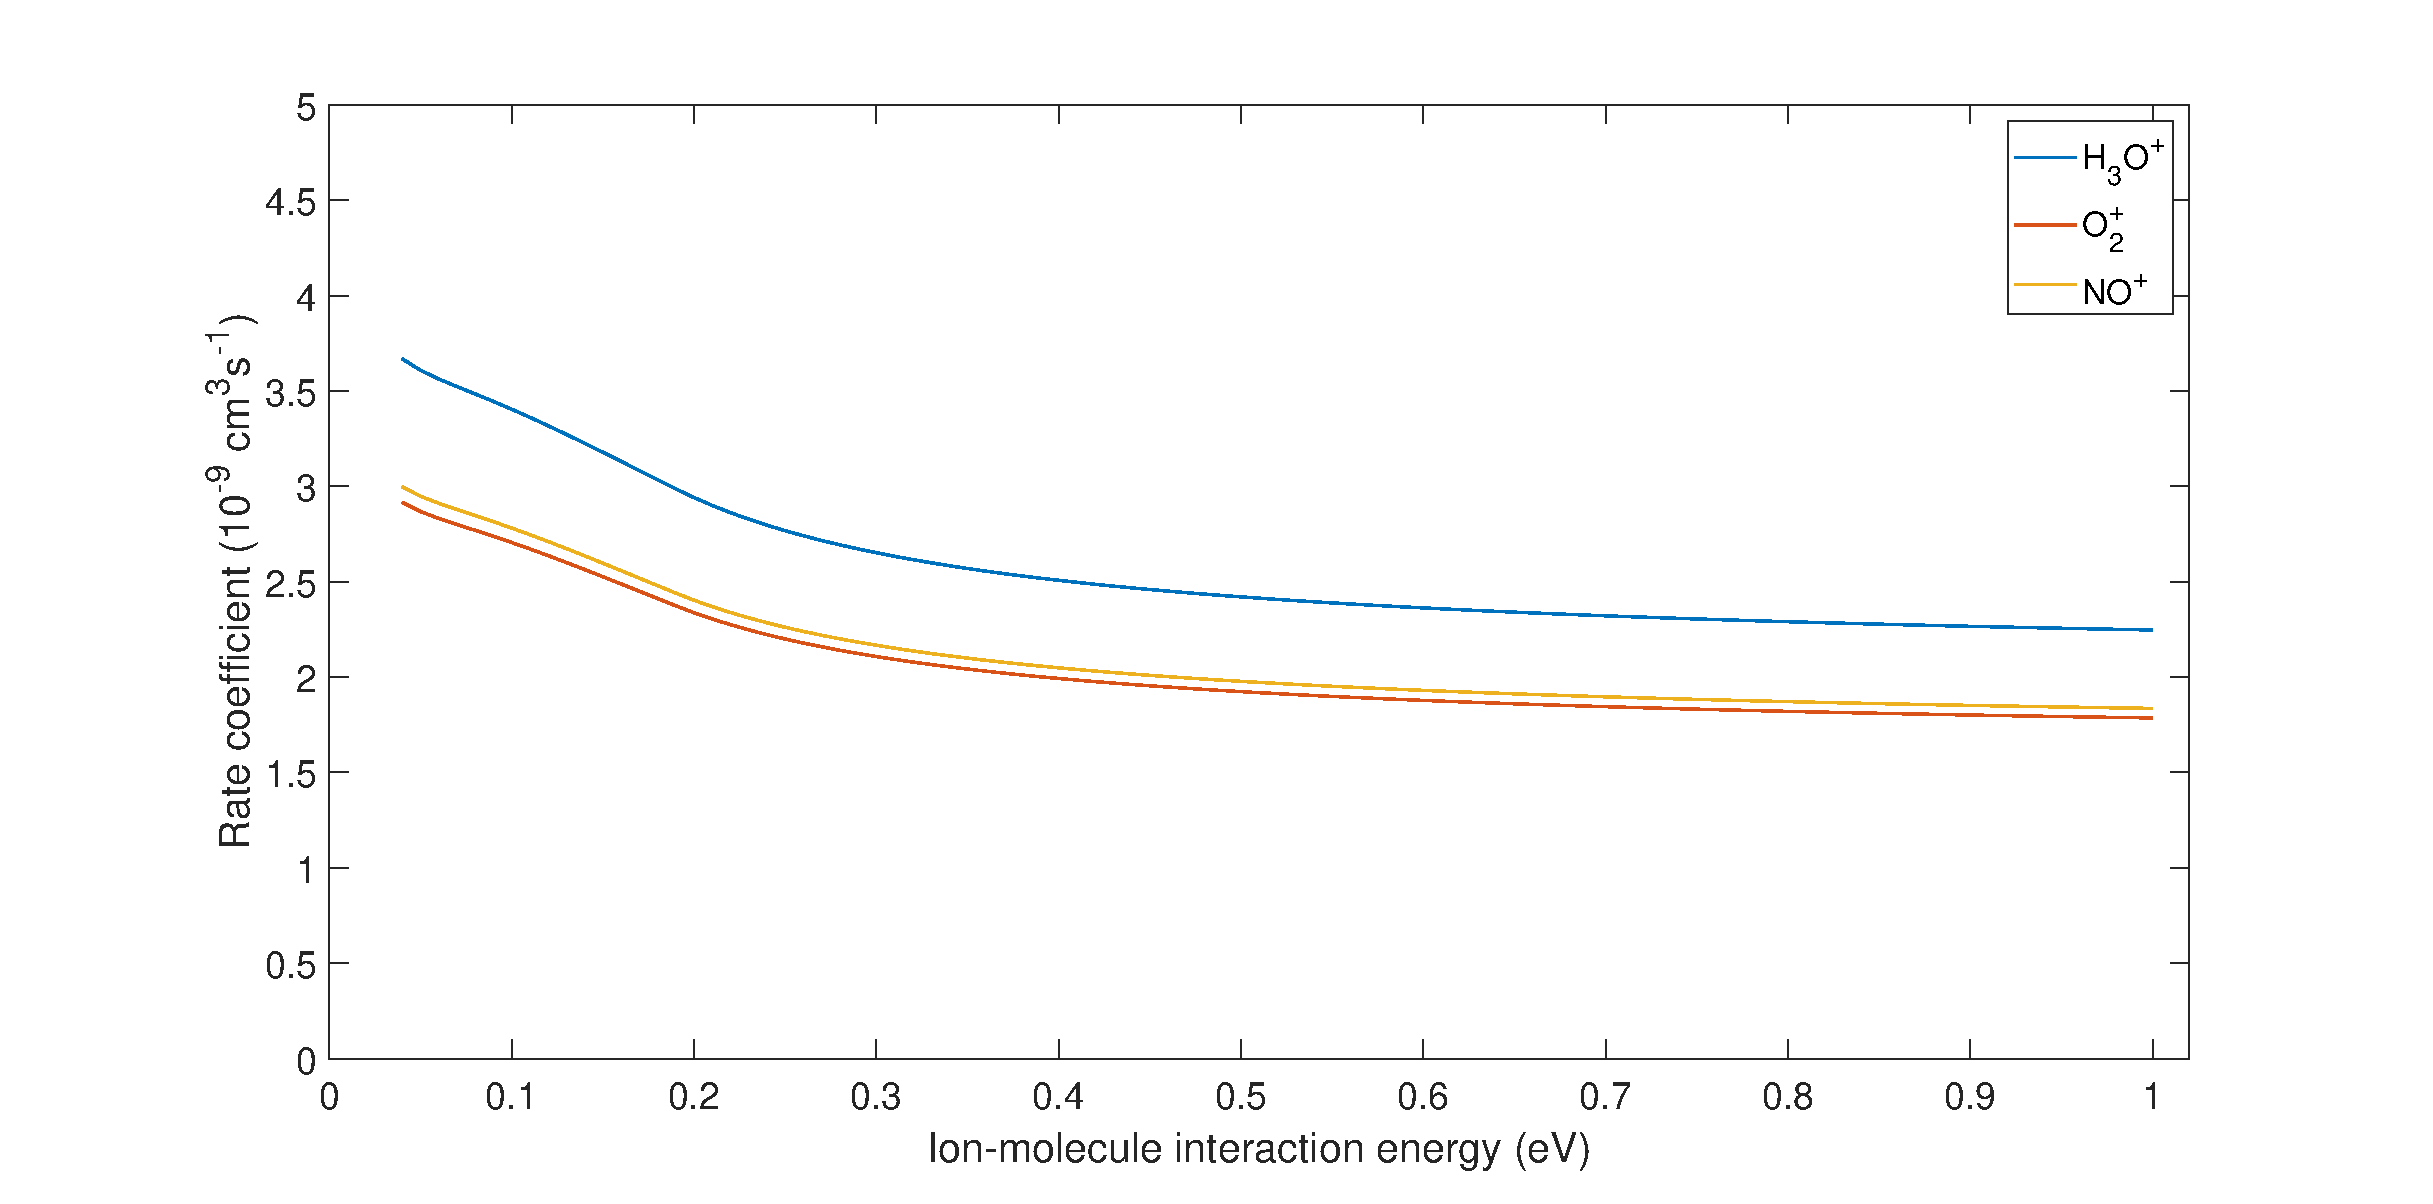
\includegraphics[width=0.9\linewidth]{pics/rate_constants_isoflurane.eps}}

\sidesubfloat[]{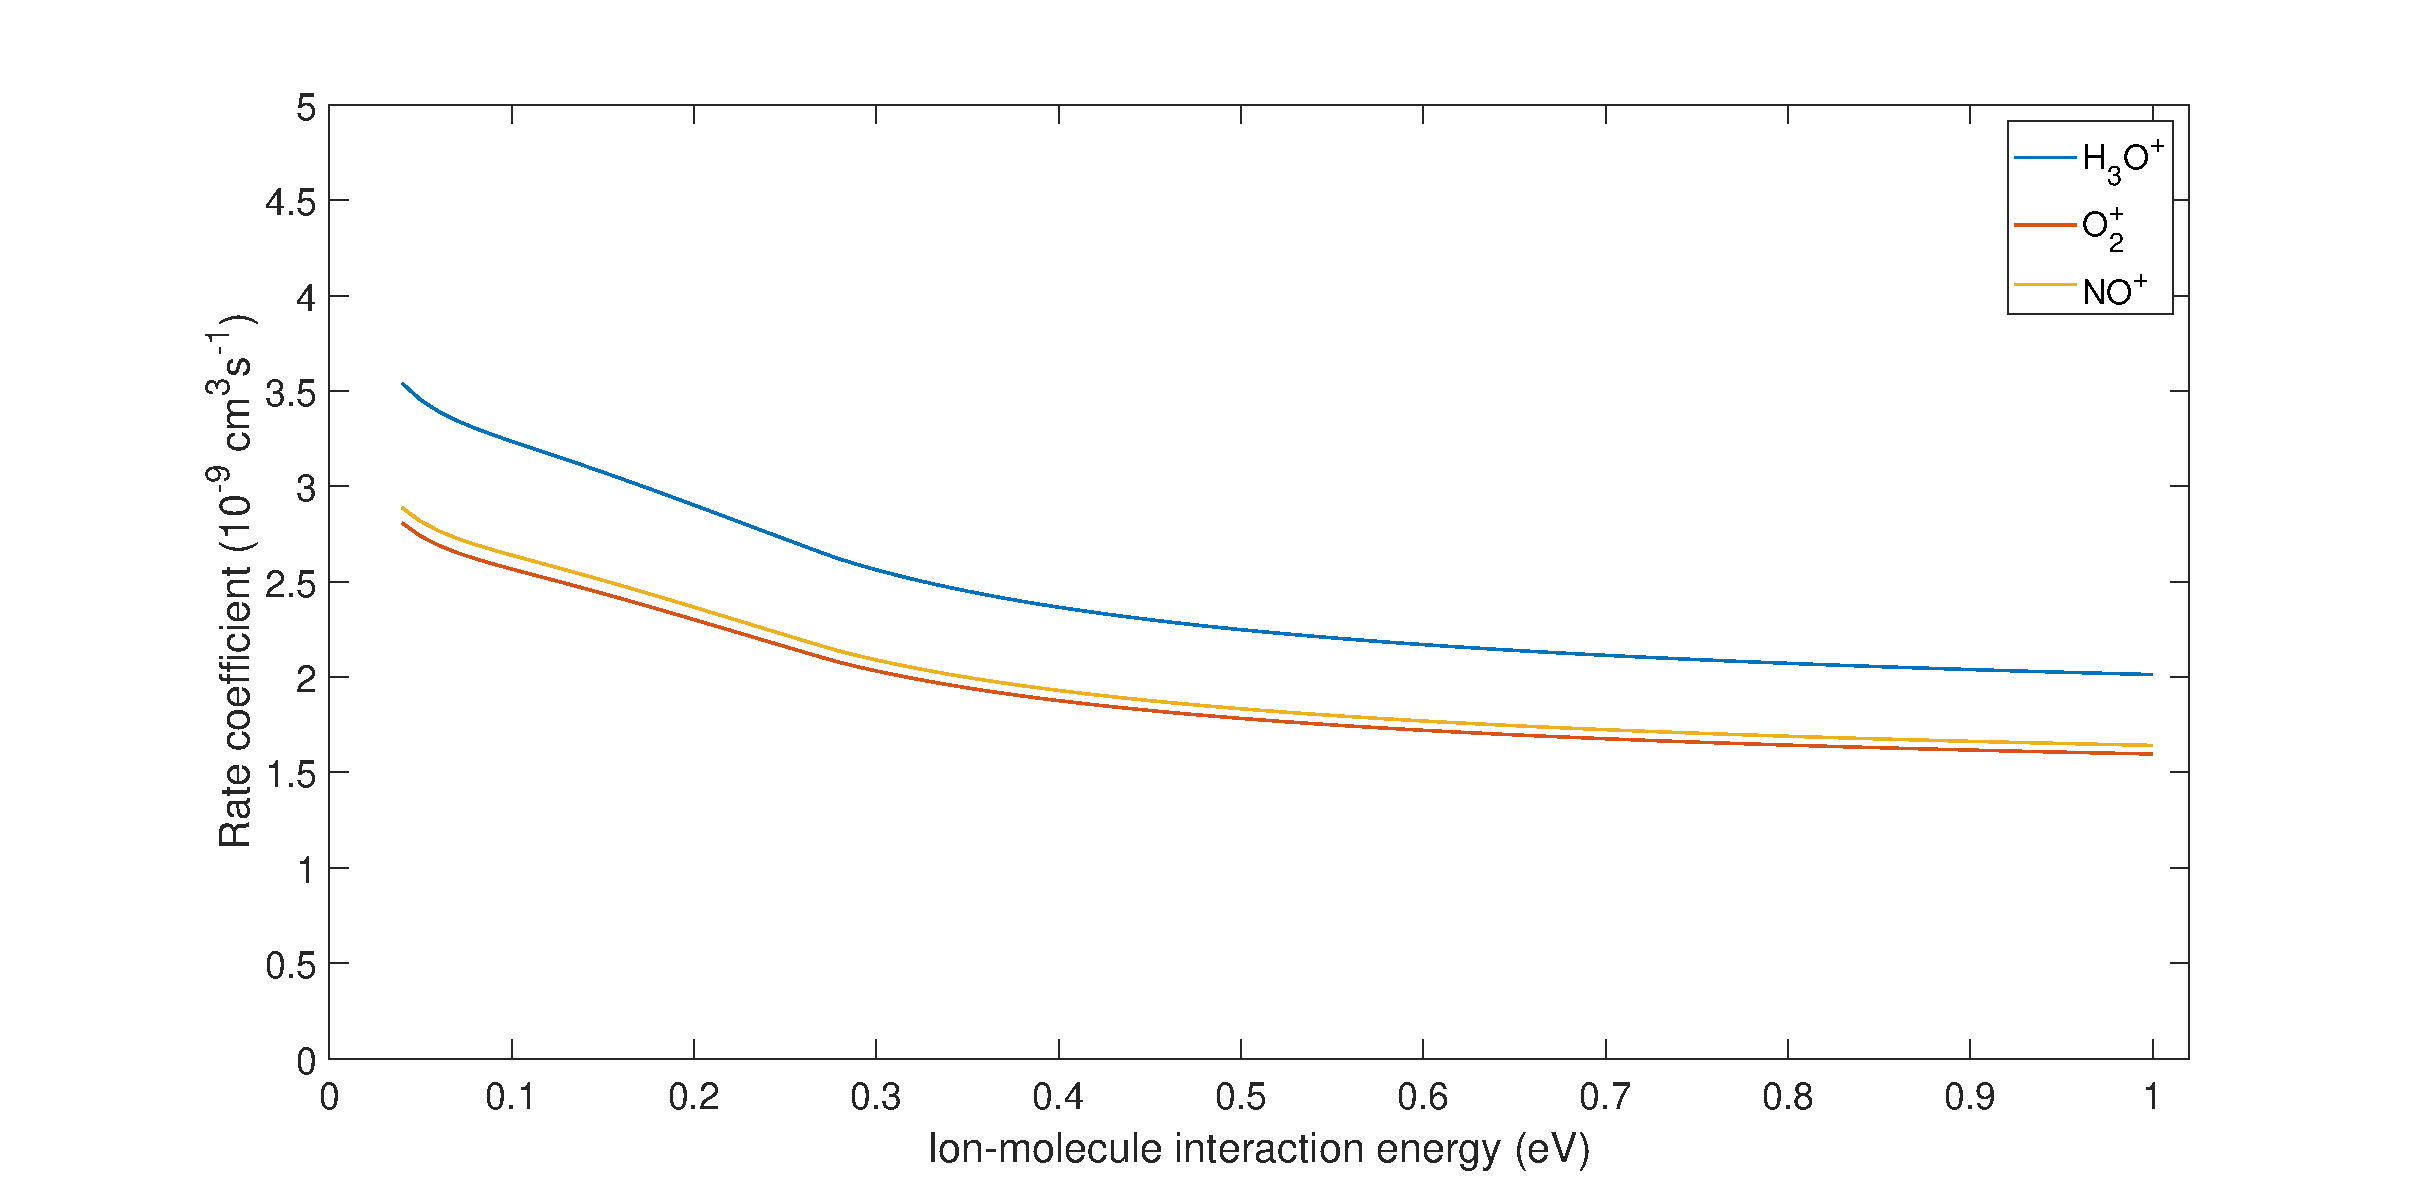
\includegraphics[width=0.9\linewidth]{pics/rate_constants_sevoflurane.eps}}
\caption{Collisional rate coefficients of (a) isoflurane and (b) sevoflurane with different reagent ions as a function of the interaction energy as predicted by the Su model \cite{su1994parametrization}}
    \label{fig:rate_iso_sevo}
\end{figure}



\section{Concerns at the moment}
There are some concerns regarding isoflurane:
\begin{itemize}
    \item It is very sensitive to humidity. In the past, people thought that the discrepancies in the PTRMS results from isoflurane measurements were due to the difference geometries of the instruments from different manufacturers, which raised doubts about the standardisation of PTRMS.
    \item There is an ion reported at m/z 163 by \cite{Wang2002SelectedSevoflurane}. The energy required for its fragmentation it is too high, around 1.8 eV.
    \item Furthermore, the ion assigned to m/z 147 does not have proper isotopic distribution (note that the scale is logarithmic and m/z 149 is not 1/3 of m/z  147)
\end{itemize}




\section{Results and discussion}
\section{Conclusions and further remarks}
















\chapter{COMPUTATIONAL METHODS: ION TRAJECTORY SIMULATIONS}
\markboth{COMPUTATIONAL METHODS}{}

Description of the computational model, experiments in DC and RF and comparison with the simulations for the reagent ions, which represent the majority of ions in the reactor.

Note this is only in the reactor and there are several more stages until the mass spectrometer which can influence the transmission of ions


\section{Introduction}

In the literature there are available some works, like for ESI with CFD \cite{doi:10.1002/jms.3519}. In the case of PTR-MS but with no scattering model \cite{ENNIS200572}

Ion funnels design parameters: see equation 7 in \cite{doi:10.1021/ac990346w}. Have a read at the whole article to refresh.


\section{Description of the model}









SIMION version ....

Montecarlo simulations

Collisional model HS1. Accounts for hard sphere collision. This model has been described in the literature \cite{appelhans2002measurement,DAHL20003,manura2008simion}. Briefly:
\begin{itemize}
\item The buffer gas is  neutral and its velocity follows the Maxwell-Boltzmann distribution\footnote[2]{From kinetic gas theory (Maxwell-Boltzmann), velocity in one dimension is normally distributed with standard deviation $\sigma_v = \sqrt{\frac{kT}{m}}$.}.
\end{itemize}


Collisions are assumed to be elastic as the only collisions accounted for are ion-neutral collisions, i.e. no proton transfer, clustering/declustering or fragmentation reactions are simulated.


The mean free path of the ions \cite{hirschfelder1954molecular}:
\begin{equation}
\label{eq:mfp}
\lambda = \frac{R T}{\sqrt{2} \pi d^2 N_A P} = \frac{k T}{\sqrt{2} \pi d^2 P}
\end{equation}
where R is the ideal gas constant, N$_A$ is Avogadro's number, T is the temperature, P is the pressure, d is the hard-sphere diameter of .... buffer gas? or sum of gas and ion?, 


\begin{figure}%[ht]
\centering
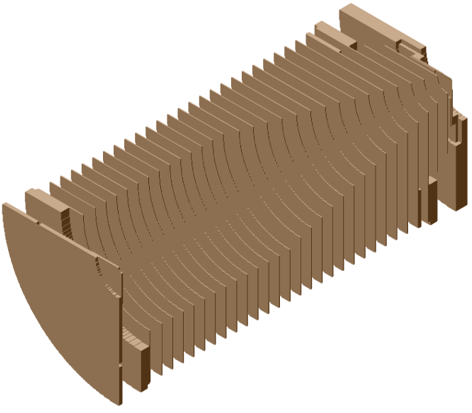
\includegraphics[width=0.7\linewidth]{pics/Reactor.PNG}
\centering
\caption{Geometry of the reactor used for the simulations in this chapter.}
\label{fig:sim_dt}
\end{figure}

\subsection{Parameters}

Table of parameters for SIMION are shown in table \ref{tb:sim}.

\begin{table}[ht]
\centering
\caption{List of parameters for the ion trajectory simulations.}
\label{tb:sim}
\begin{tabular}{lcc}
\toprule
\textbf{Parameter}	 &\textbf{Value}	&\textbf{Units} \quad\\ \midrule 
m/z           & 19, 37, 55, 73    	&Da?    				\\
ToB				& 	0.05				& $\mu$s\\
N				& 20000 			&ions \\
Coulombic Factor			&3$\times$10$^5$				&- \\
Drift voltage			&15-? 		&V \\
E/N (DC mode only)			&- 		&Td \\
Pressure			&1 				&mbar \\
Temperature			&100-150? 		&$^{\circ}$C \\
More parameters?? & & \\
\bottomrule
\end{tabular}
\end{table}

The time of birth (ToB) and the Coulombic factor are set to the values that yield a current of roughly 1 $\mu$A through the entry plate of the drift tube:
\begin{equation}
I = \frac{\Delta Q}{\Delta t} = \frac{3\times10^5 e}{0.05\, \mu s} = 0.96\, \mu A
\end{equation}



\subsection{Validation}
To validate the model and the parameters I compared the simulated results with the current measured at the exit plate with a picoammeter 








\section{Results and discussion}


\subsection{Drift time of ions in DC and RF mode}
Do some isolated ions flight at different voltages to measure drift times and compare to 1\slash V. Also to compare DC and RF modes. (N=1000, ungrouped)




 Files:
 \begin{itemize}
 \item DC mode: \verb|10-42-26_25-July-2018_simulation|
 \item RF mode: \verb|21-43-27_25-July-2018_simulation|
 \end{itemize}

 This can also be thought in terms of the drift voltage: t$_d$ is  proportional to 1\slash V$_d$, as E is proportional to V$_d$. Plotting the drift time can be a quick test..........

 Figure \ref{fig:td} shows the drift time of ions of m/z 19, 37, 55 and 73 at different drift voltages together with the 1/V fit from \ref{eq:tdfit}.
 \begin{equation}
t_d(V_d) = \frac{a}{V_d+c}+b\footnote[2]{It should be something like: $ m \frac{d^2x}{dt^2} = eE + C_1\frac{dx}{dt}$ 
(damping term = b in my stuff) 
$ + C_2\frac{dx}{dt} $ 
(flowing term = c in my stuff)
and  $  m \frac{d^2x}{dt^2} = 0 $ 
because it is a steady state. I should look for this in the Tolmachev papers, he does something similar. In \cite{TOLMACHEV200031} there is an expression for 
$dv/dt$
. Also have a look at \cite{TOLMACHEV2003155}. I can also separate the DC and RF this way and get different fits for DC and RF modes. Also check (commented link) %http://www.binep.ac.ru/Publics/Pdf/1997_p013_e.pdf
 }
 \label{eq:tdfit}
 \end{equation}















\begin{figure}%[h]
\begin{center}
\sidesubfloat[]{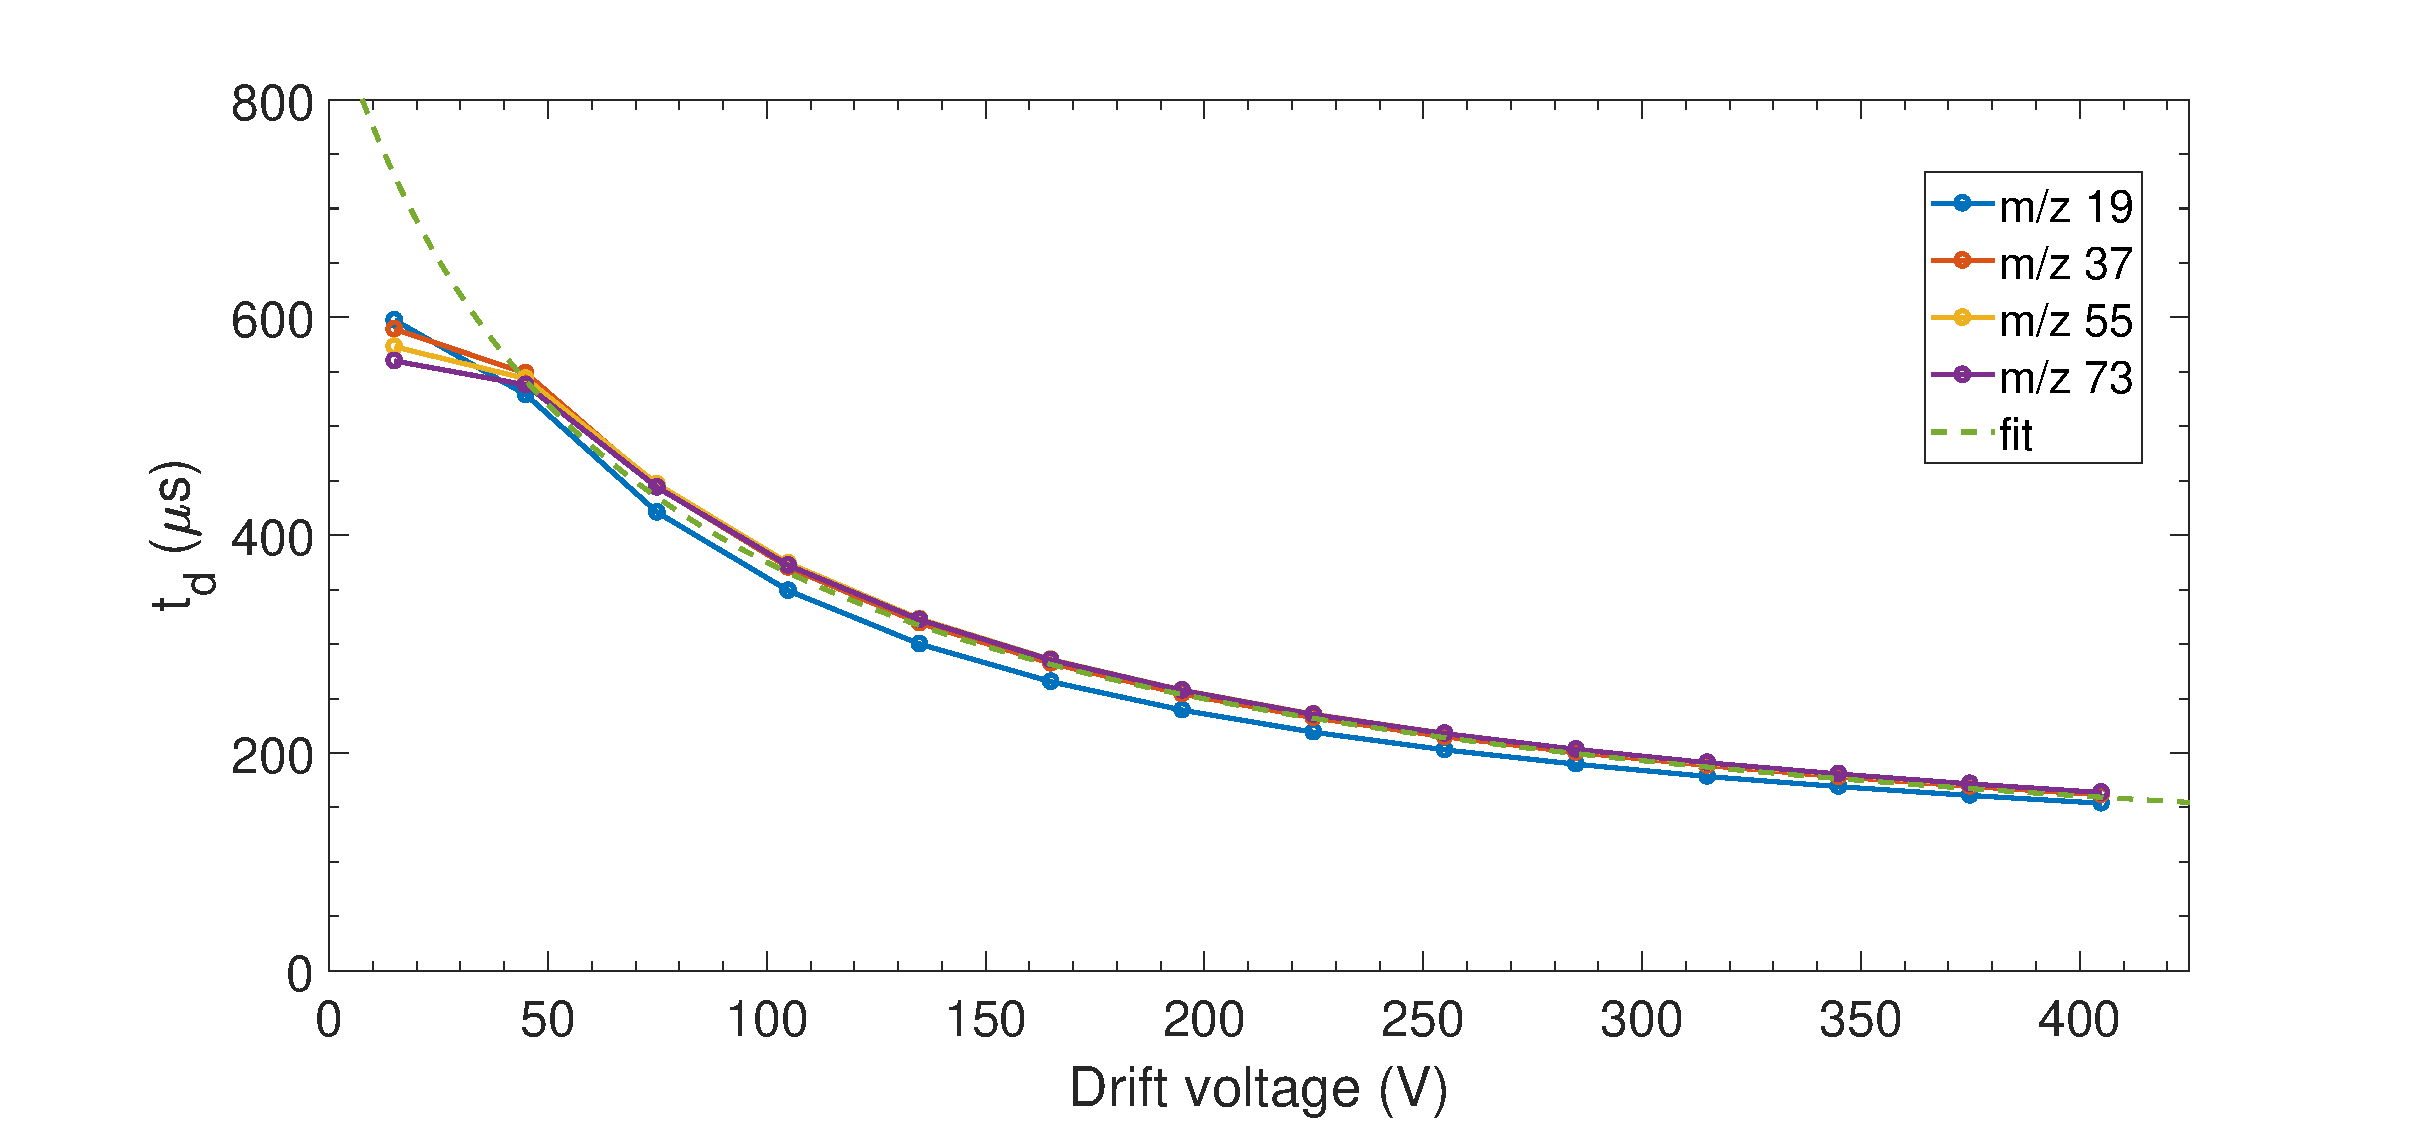
\includegraphics[width=0.9\linewidth]{pics/td_HS1.eps}\label{fig:td_DC}}

\bigskip
\sidesubfloat[]{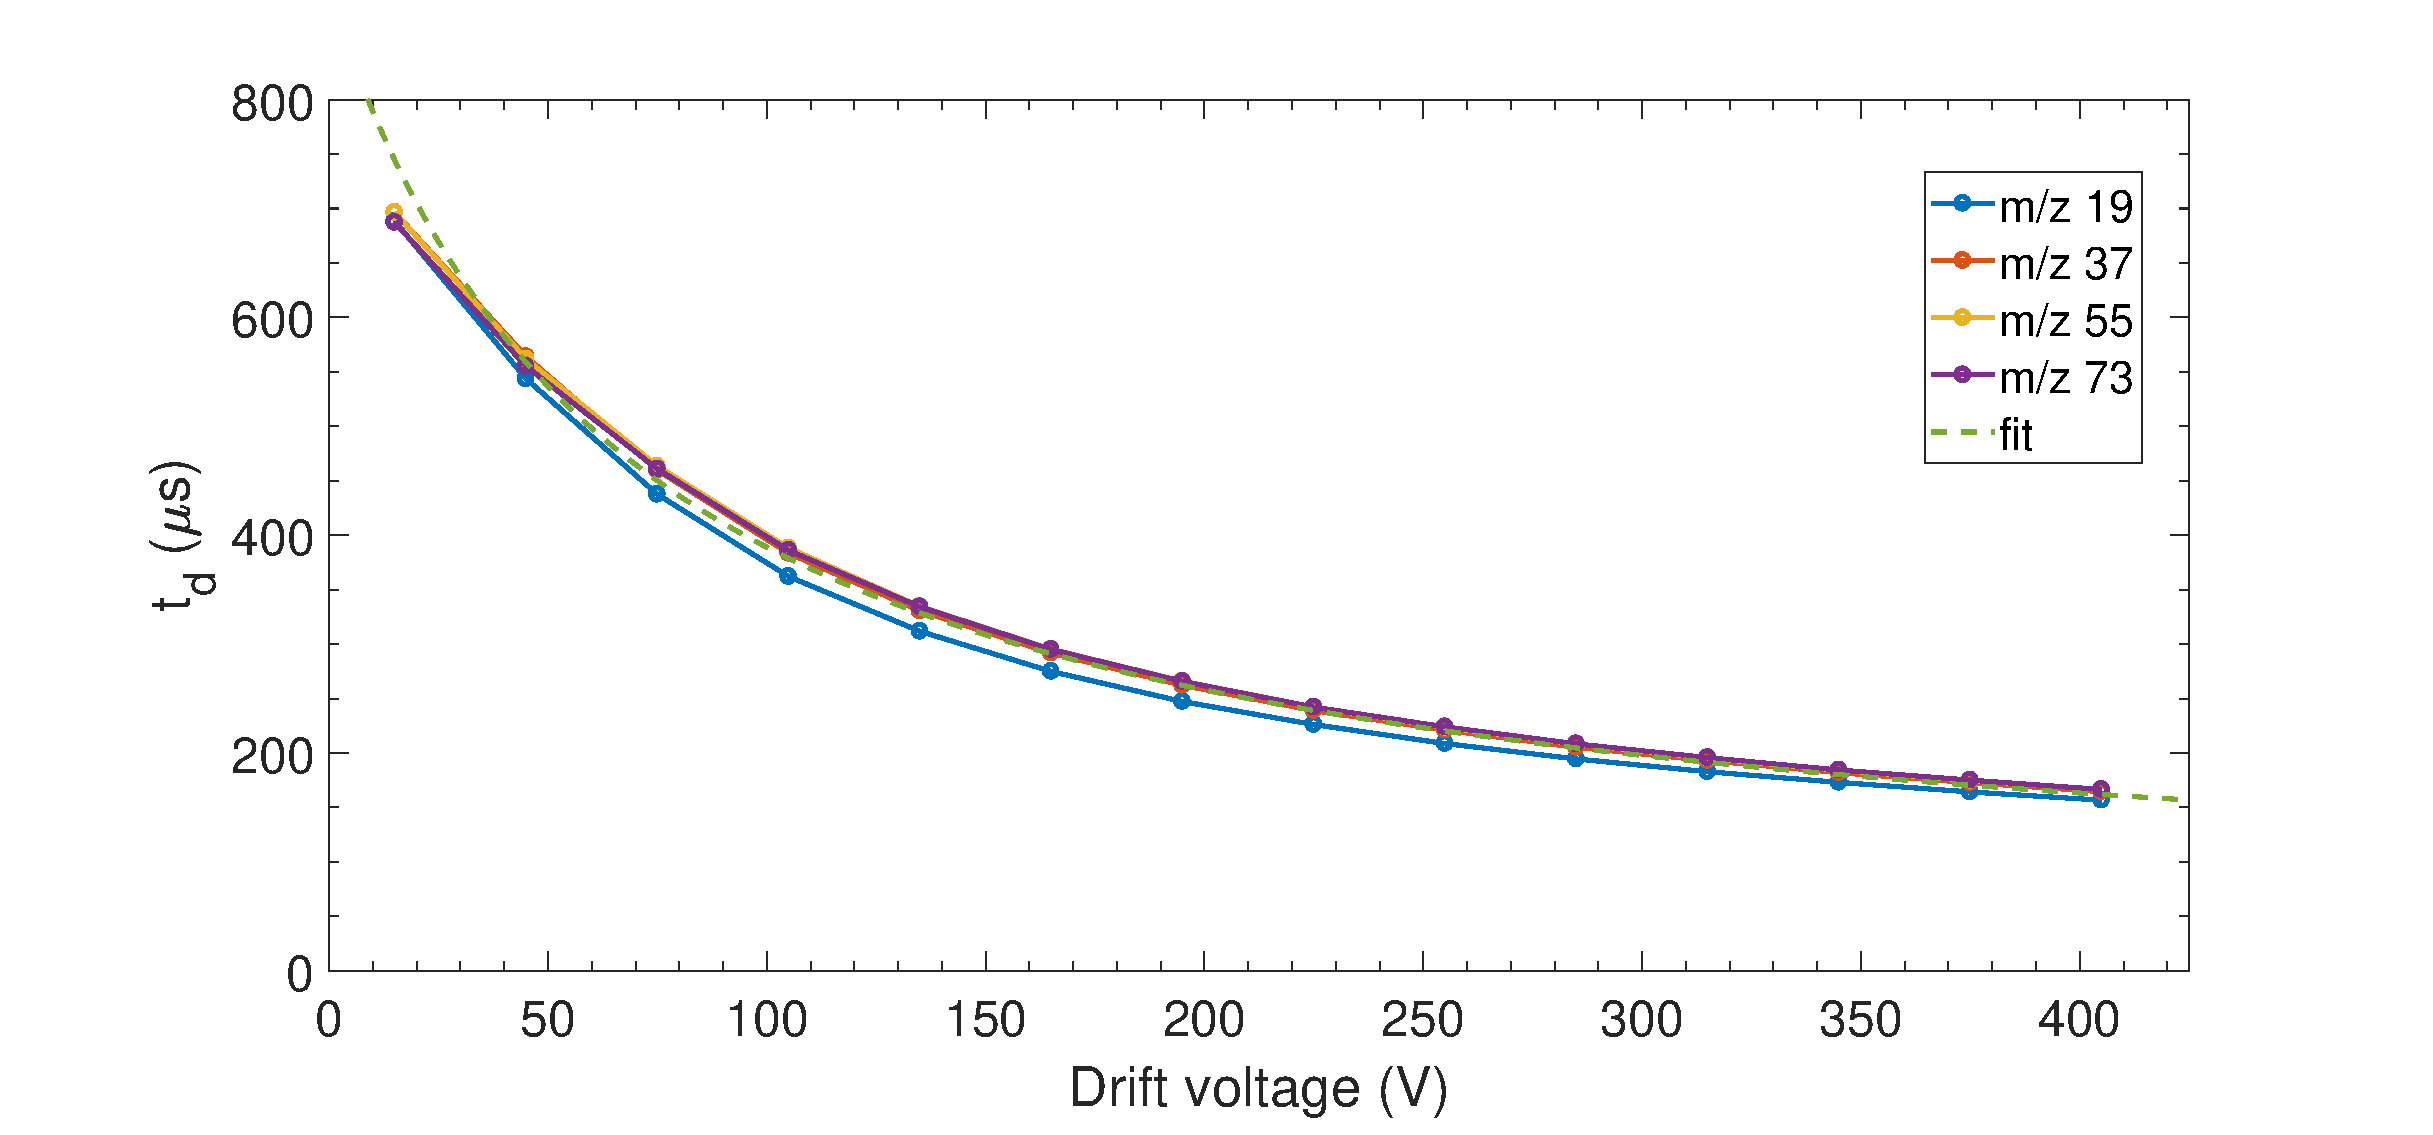
\includegraphics[width=0.9\linewidth]{pics/td_RF_HS1.eps}\label{fig:td_RF}}
\end{center}
\caption{Plot of the drift time, t$_d$, as a function of drift voltage for (a) DC mode and (b) RF mode. \textbf{THIS DATA IS OLD. THE NEW ONE NEEDS TO BE PLOTTED}}\label{fig:td}
\end{figure}







\subsection{Collisions in DC and RF mode}
I can also have a look at the number of collisions in each mode.
I can plot the kinetic energy vs the number of collisions for each mode


Compare DC and RF. Calculate the difference (in total and \%) of the collisions for both modes. This is shown in figure \ref{fig:col}.









\begin{figure}%[h]
\begin{center}
\sidesubfloat[]{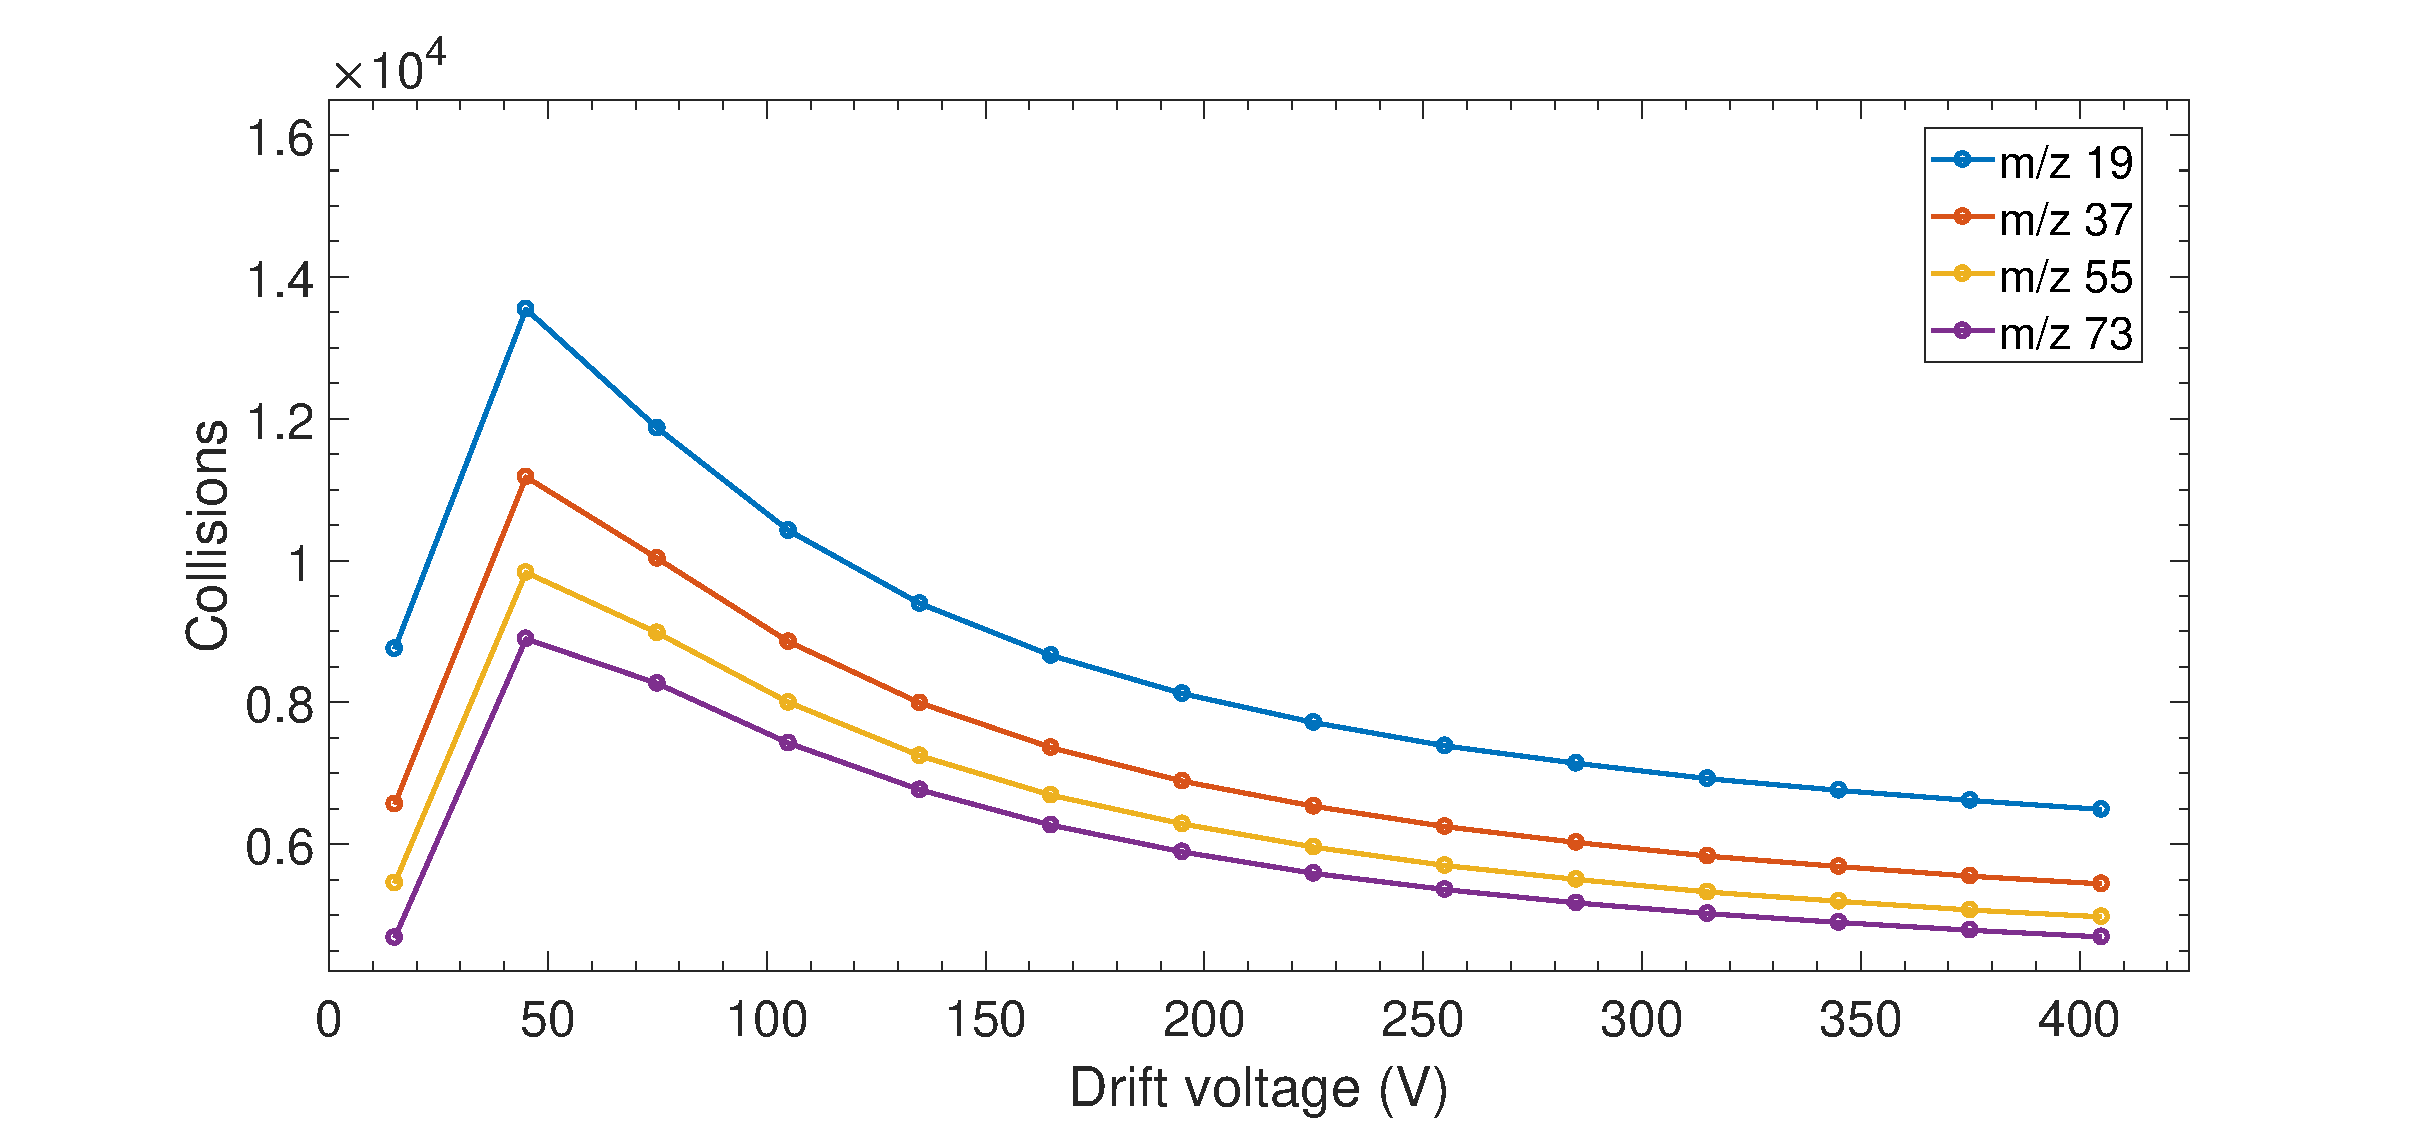
\includegraphics[width=0.9\linewidth]{pics/collisions_DC.eps}\label{fig:col_DC}}

\bigskip
\sidesubfloat[]{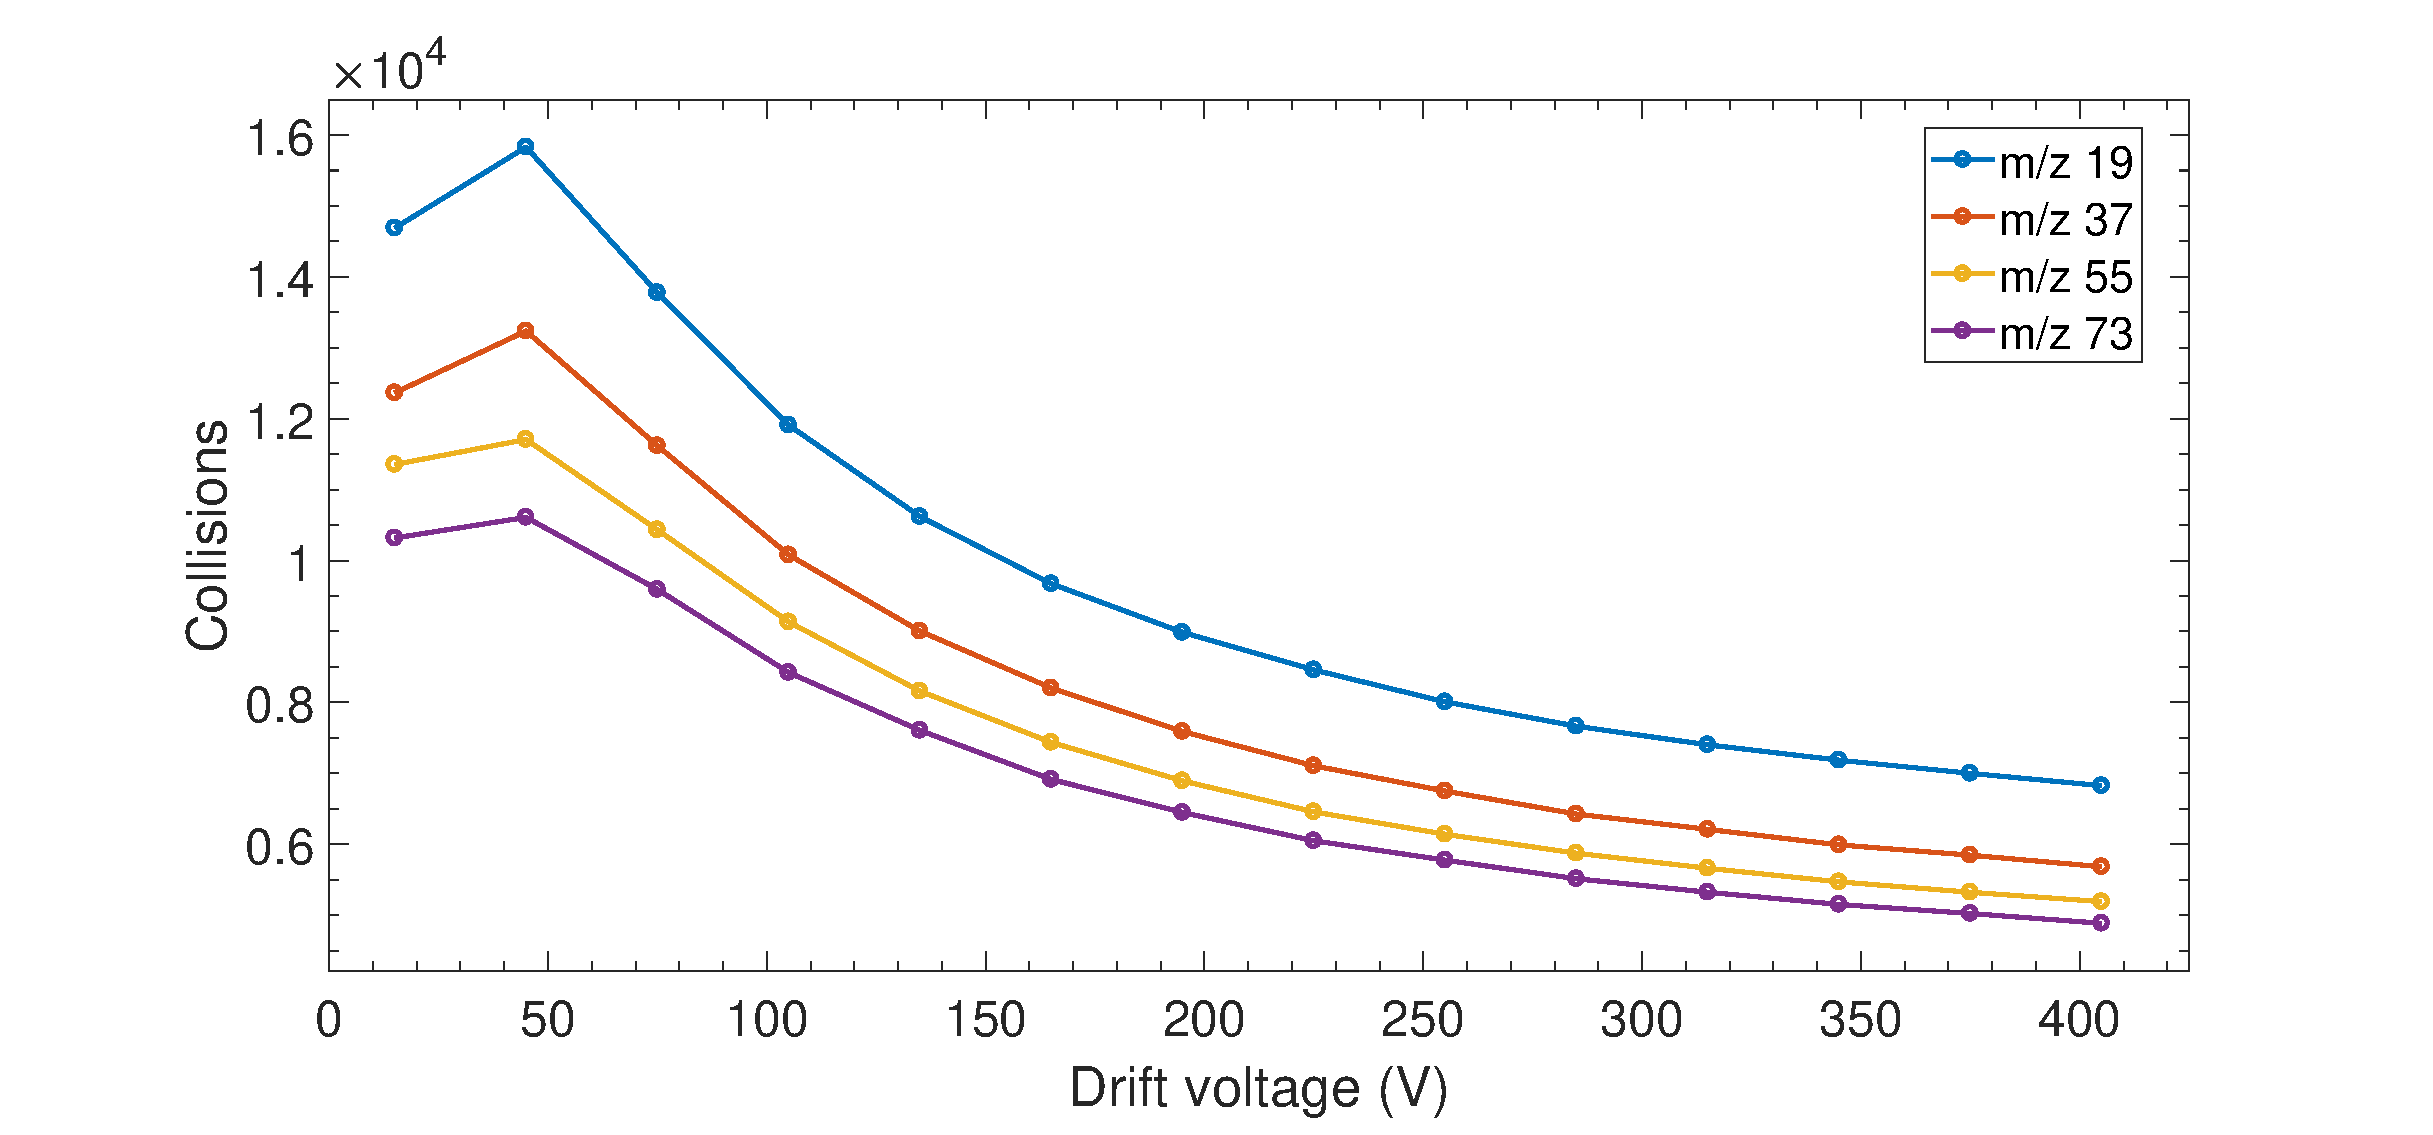
\includegraphics[width=0.9\linewidth]{pics/collisions_RF.eps}\label{fig:col_RF}}
\end{center}
\caption{Plot of the average number of collisions that every ion undergoes as a function of drift voltage for (a) DC mode and (b) RF mode }\label{fig:col}
\end{figure}













\subsection{Different configurations of the RF field}

The RF field voltage supplied to each of the plates, A$_{RF,n}$, can defined as:
\begin{equation}
A_{RF,n} = A_0\,sin\left(2 \pi f t + \phi_n    \right)
\label{eq:rf}
\end{equation}
\begin{equation}
\phi_n =  \frac{2 \pi n  }{n_p}
\label{eq:phase}
\end{equation}
where A$_0$ is 100 V (i.e. 200 V peak-to-peak), f is the linear frequency of the RF field (760 kHz), n indicates the n$^{th}$ plate, n$_p$ is a parameter to control the phase difference, t is the simulation time (in $\mu$s in SIMION, so the frequency must be converted to MHz), etc

Note that n$_p\,=\,2$ in the typical configuration of the RF field. This means that adjacent plates have opposite polarities, i.e. a phase difference of $\Delta\phi = \pi$, with $\Delta\phi = \phi_n - \phi_{n-1}$.

Note that for n$_p\,>\,2$ the RF field becomes a travelling wave, as opposed to a standing wave for n$_p\,=\,2$.

\begin{itemize}
\item Poner screenshots de ejemplos con n$_p$ 2,3,4 etc. de la superficie equipotencial y de la trajectoria de iones
\end{itemize}


\textbf{TO INCLUDE HERE: }
\begin{itemize}
\item simulations of transmission at low E/N (20 or 50V) for different values of np
\item Compare the different collisional models: the viscous model shouldn't take long to simulate. Pros and cons of each model: time consuming, precision, etc..
\item Do studies of average drift velocity as a function of E or E/N and as a function of the m/z of the ions (19,37,55,73) in DC and RF mode (can also be done for different values of n$_p$). With this, mobility can be calculated for each case (plot v$_d$ vs E)
\end{itemize}



\subsection{Calculation of the mobility of the reagent ions as a function of the E/N}
Run simulations and get v$_d$ as a function of E/N to get \acrshort{kk} from \ref{eq:vd}.
\begin{itemize}
\item Can I get the drift velocity along the whole reactor? Is it possible to get the acceleration?
\item Compare the ion mobility with the one in RF mode. Is it the same? Is it constant in any of the cases?
\item Can I extract (E/N)$_{effective}$ from this? (maybe I can explain this with a change of mobility or similar) (I could also just divide the equations)
\end{itemize}
 
Something else that I can do is to calculate the drift velocity in the first and second half of the stack in RF mode. 
\begin{itemize}
\item Does it change dramatically?
\item Compare the ion acceleration in the first and the second half of the stack to study RF acceleration.
\item Compare the drift velocity with the change in velocity with the RF mode (200V in 1/760kHz). Is it comparable?
\end{itemize}

\subsection{Flight path of the ions}
In RF mode the ions undergo more collisions. I can try to find a way to measure the travelled distance in RF and DC modes and compare them.




\subsection{Transmission as a function of the drift voltage}









To have a better idea of the transmission I considered that the number of ions that reach the exit plate are proportional to the ions transmitted through the exit aperture towards the differential pumping stage. The main reason for using the ions that reach the exit plate instead of the ones that go through the exit aperture is that it is more time efficient to use the former as the area of the exit plate is much bigger than that of the aperture.

The transmission, T, is calculated as a percentage following equation \ref{eq:sim_i}:
\begin{equation}
T = \frac{N_{exit}}{N_{f}} \times 100
\label{eq:sim_i}
\end{equation}
where N$_{exit}$ is the number of ions that hit exit plate from those flown, N$_f$. The averaged transmission is calculated following equation \ref{eq:sim_ia}:
\begin{equation}
T_{average} = 100 \times\frac{\sum_{i=1}^4 N_{exit,i}}{\sum_{i=1}^4 N_{f,i}} = \frac{1}{4}\sum_{i=1}^4T_i
\label{eq:sim_ia}
\end{equation}

Files:
\begin{itemize}
\item DC mode: \verb|16-35-24_09-January-2019_simulation-DC transmission-HS1 model| (1000 ions)
\item RF mode: \verb|14-46-57_27-April-2018_simulation|
\end{itemize}


Figure \ref{fig:sim} shows the transmission study for DC and RF modes for hydronium and the first three water clusters (N=20000, grouped, factor = 10$^6$)

Transmission is mass-dependent in RF mode while it is not in DC mode. 

Transmission increases with the drift voltage in all cases.

This low-mass cut-off of RF funnels has been reported in the literature already \cite{Chung123}



\begin{figure}%[h]
\begin{center}
\sidesubfloat[]{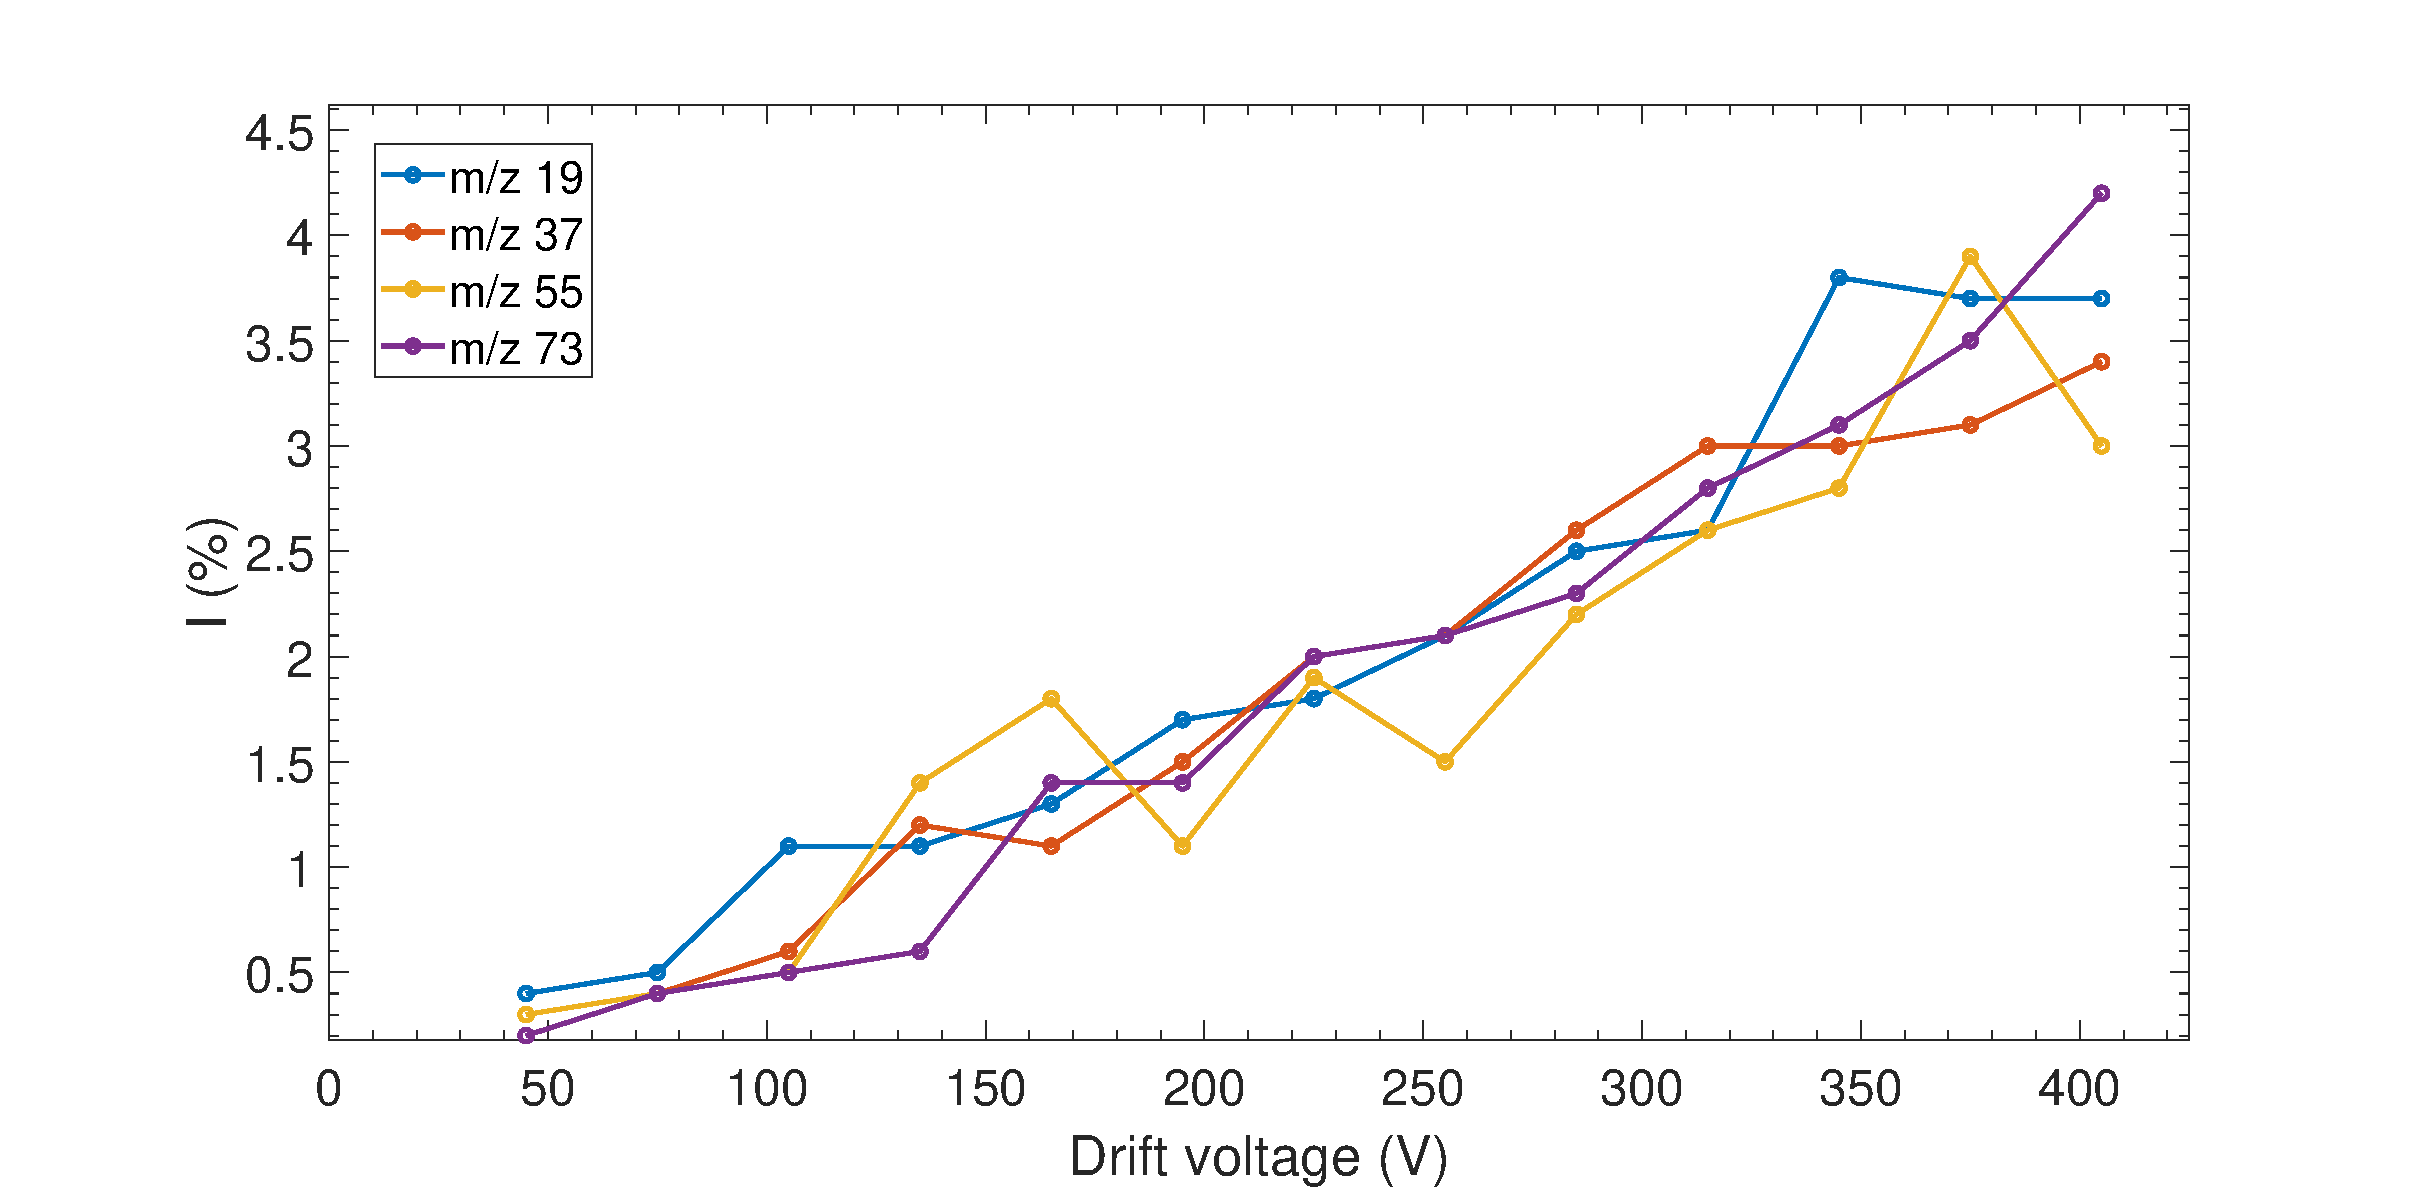
\includegraphics[width=0.8\linewidth]{pics/DC_HS1_1000ions.eps}\label{fig:sim_DC}}

\sidesubfloat[]{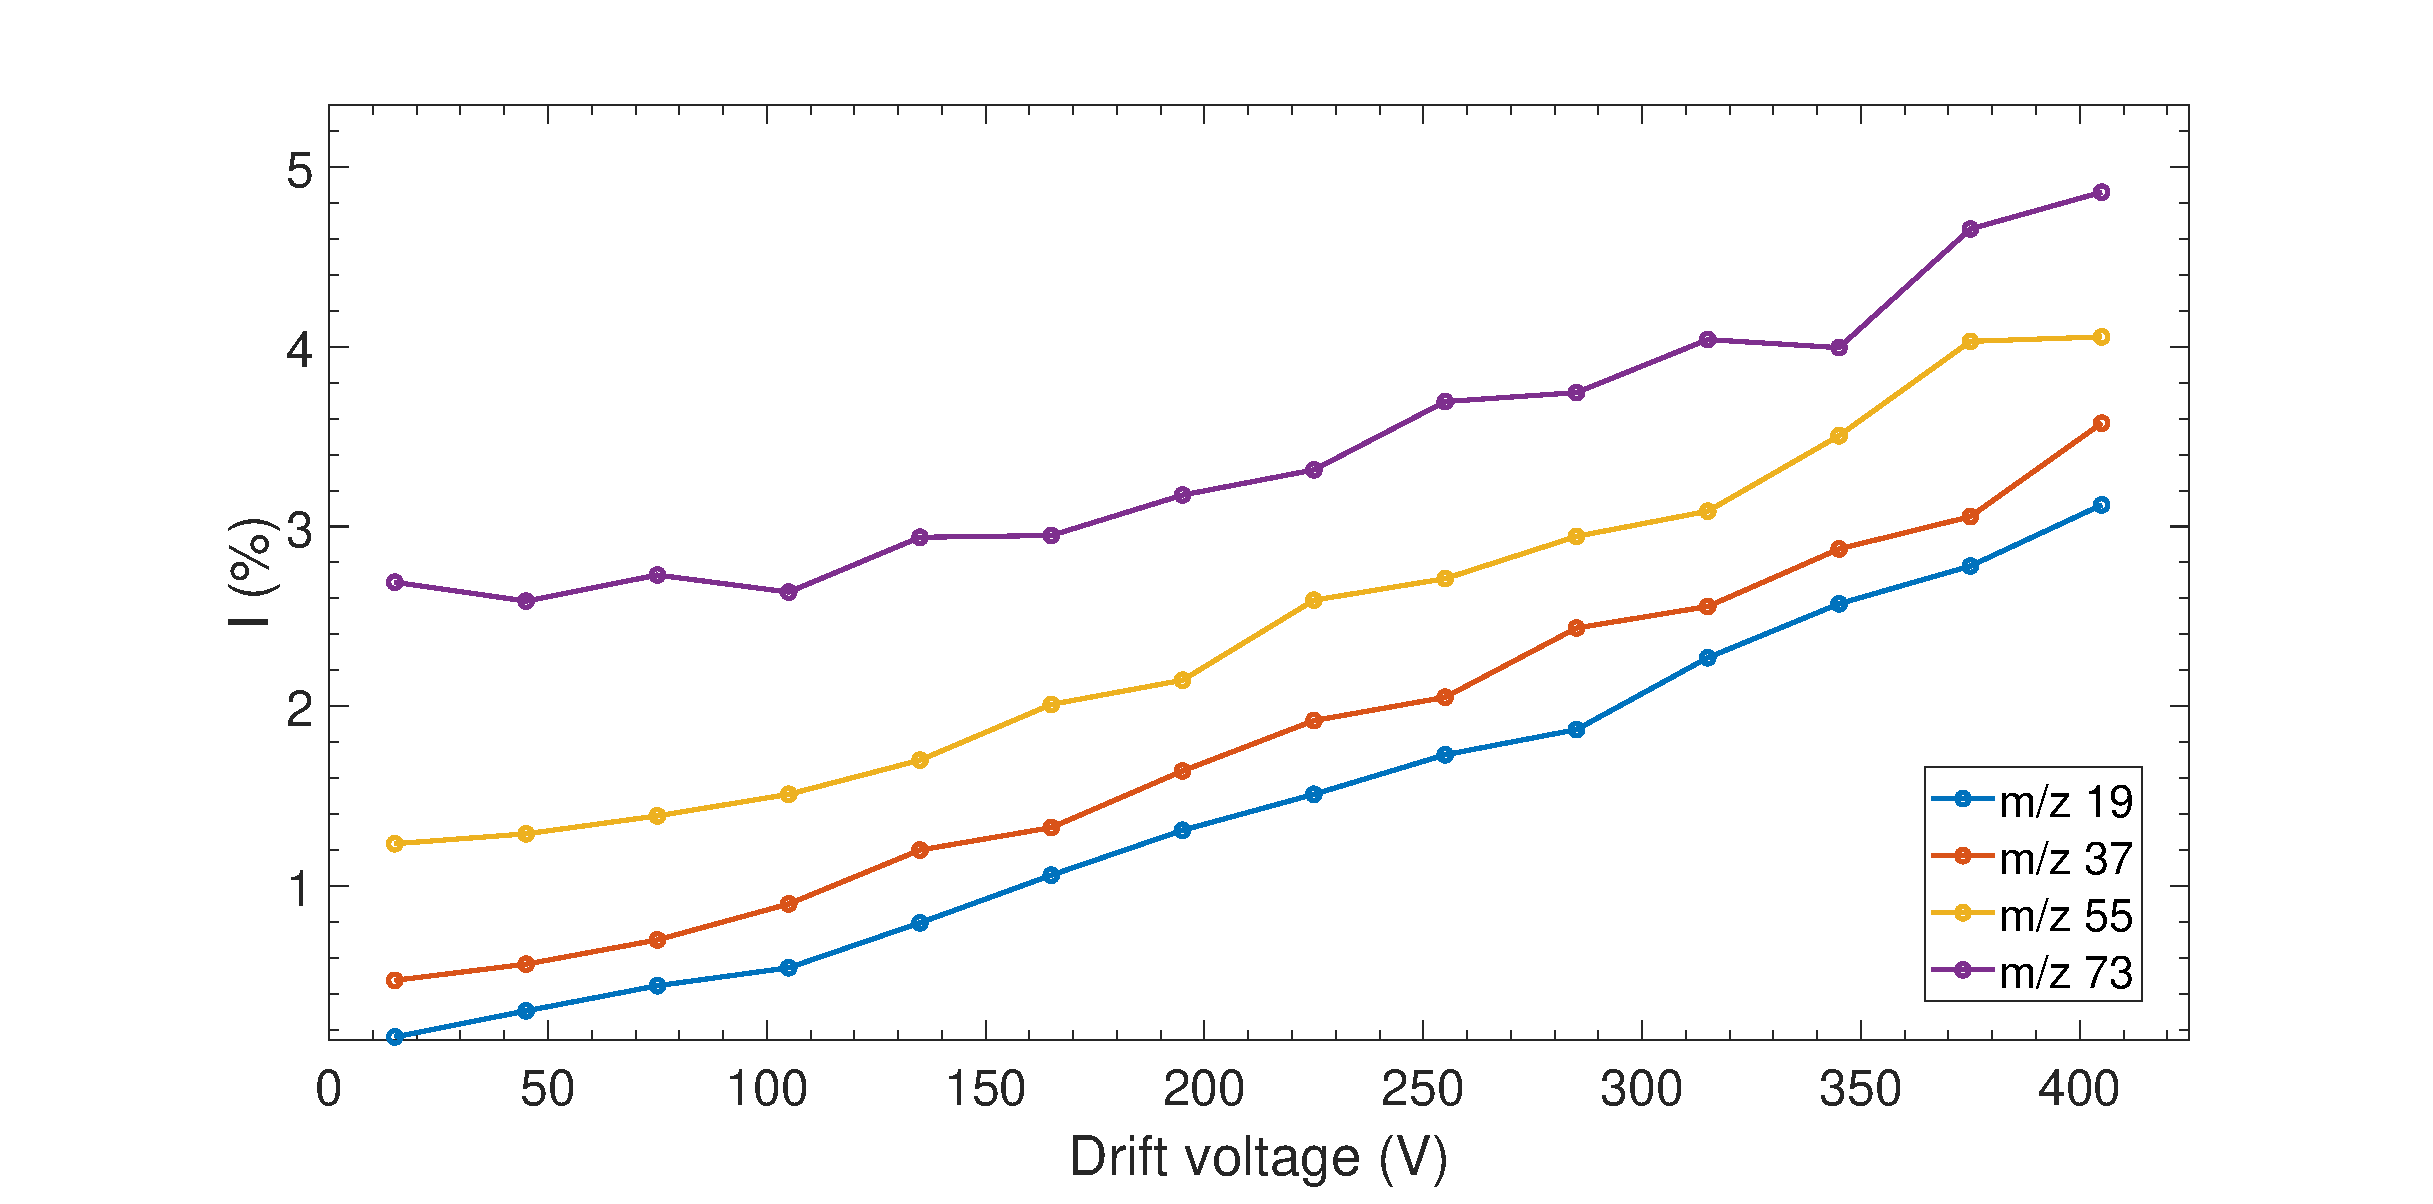
\includegraphics[width=0.8\linewidth]{pics/RF_HS1_20000ions.eps}\label{fig:sim_RF}}

\sidesubfloat[]{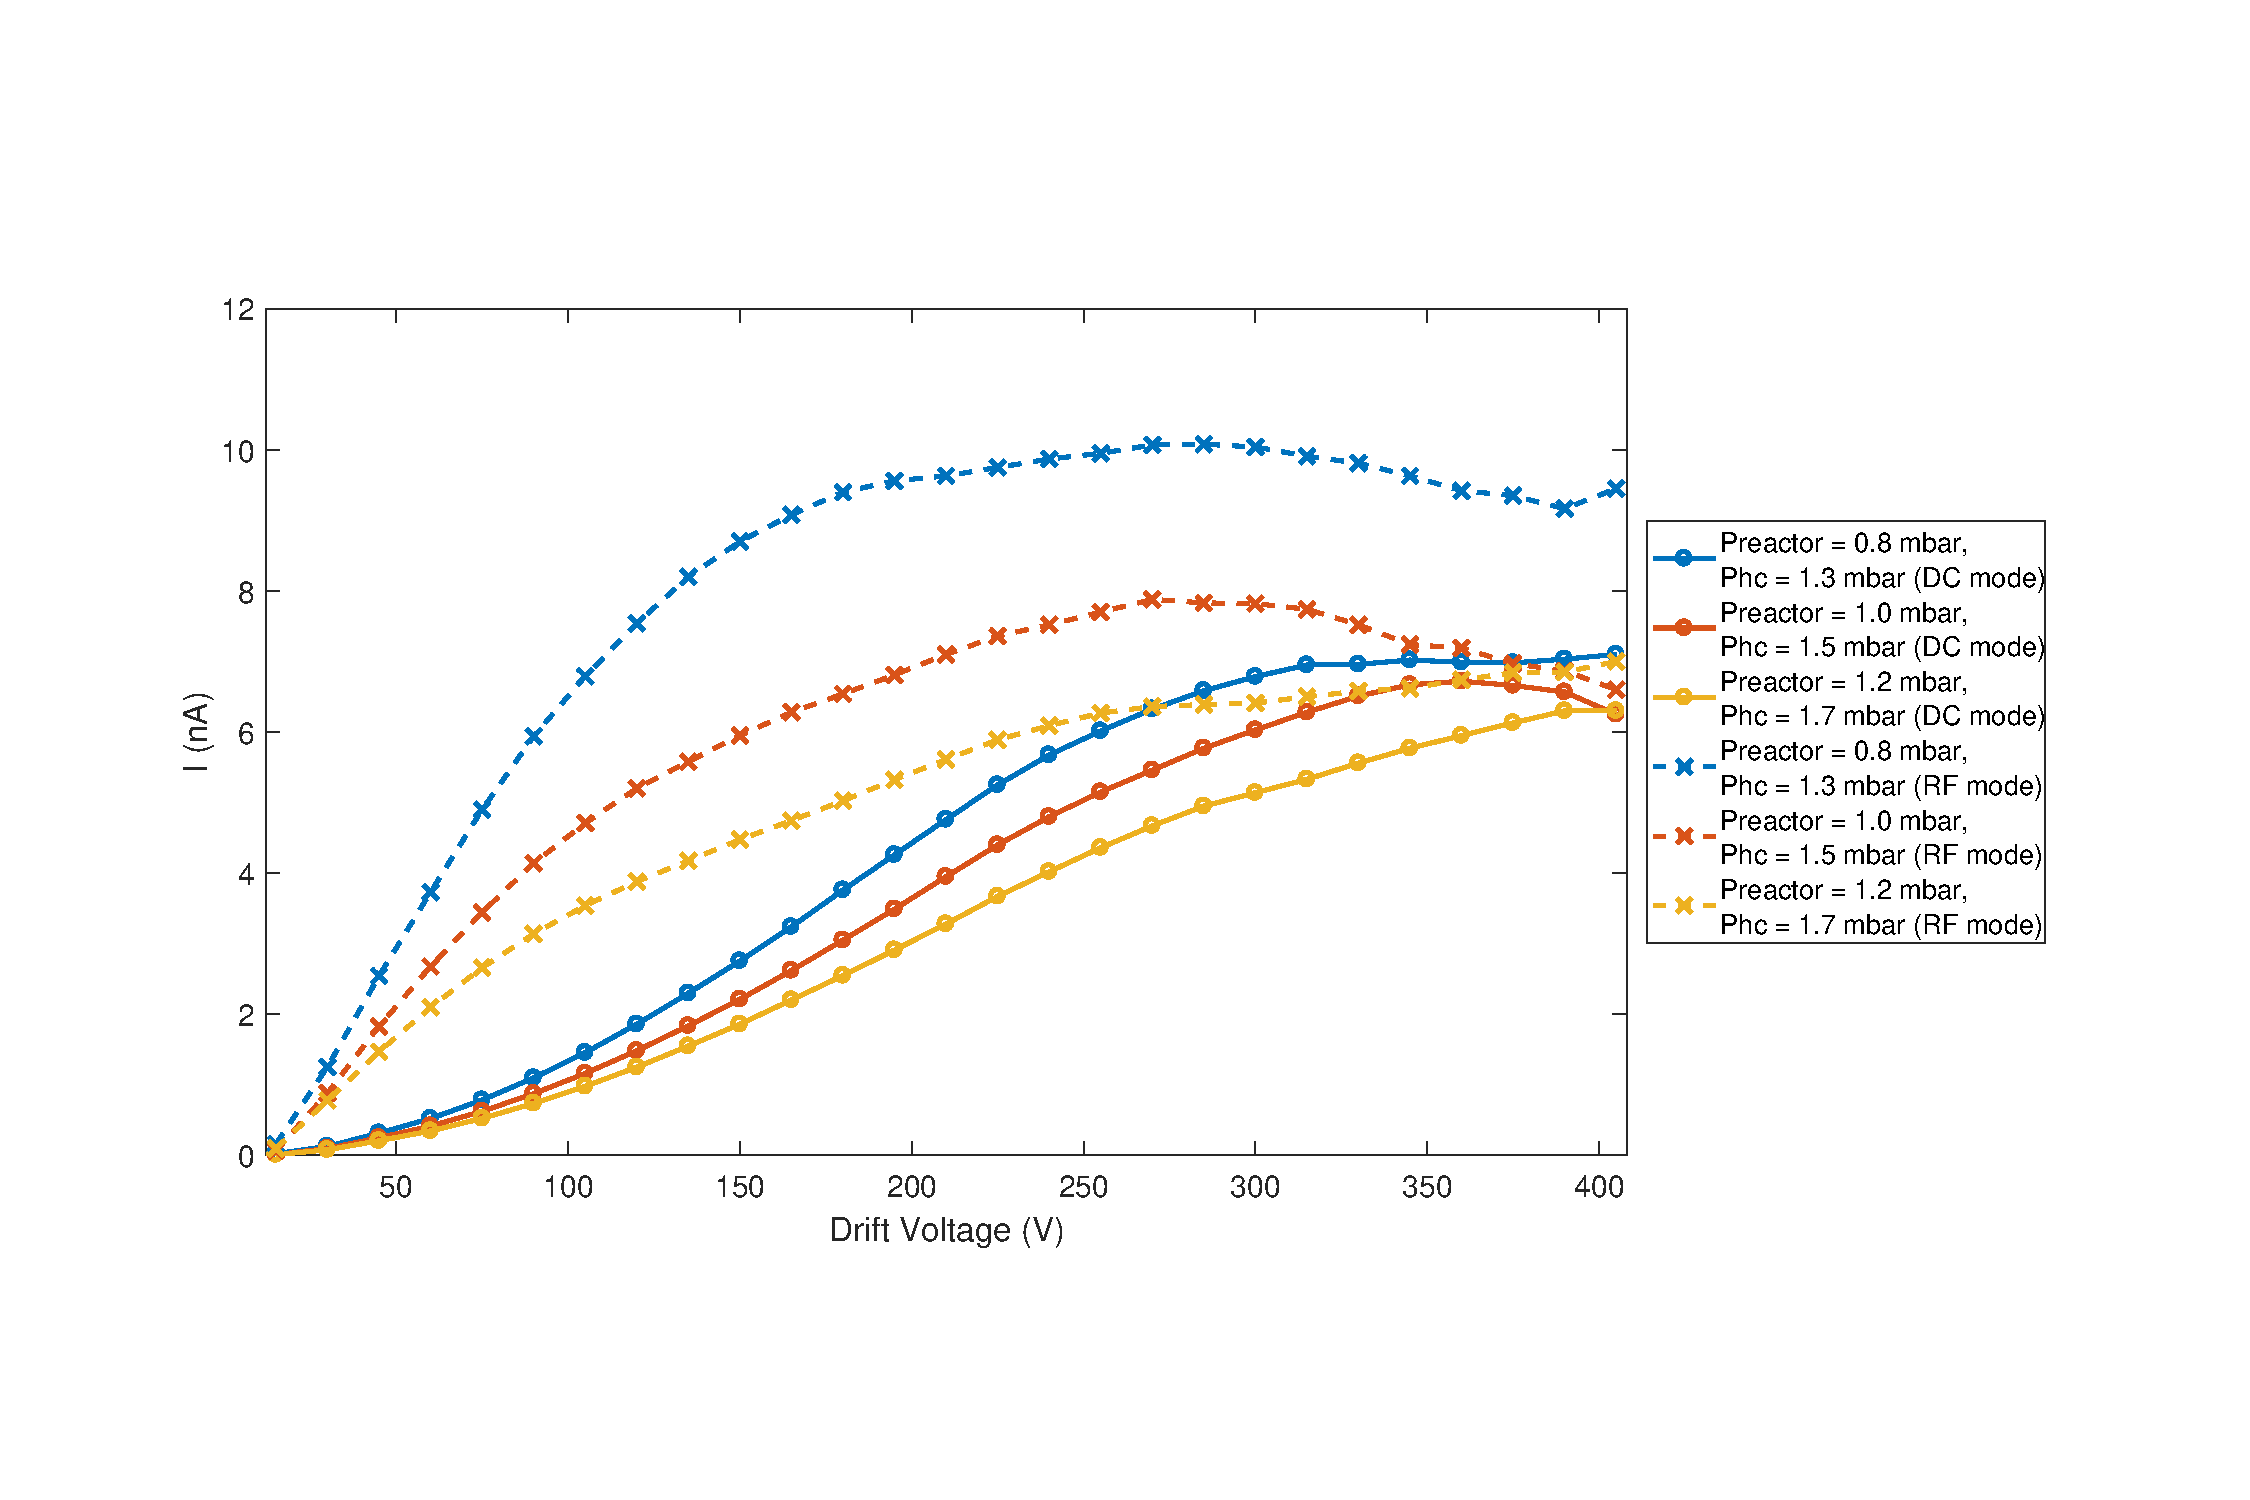
\includegraphics[width=0.8\linewidth]{pics/transmission_p.pdf}\label{fig:current_plot}}
\end{center}
\caption[Percentage of ions that reach exit plate as a function of the drift voltage for hydronium and the first water cluster ions]{Percentage of ions that reach exit plate as a function of the drift voltage for hydronium and the first water cluster ions. HS1 model, 1000 ions for DC mode and 20000 ions for RF mode.}\label{fig:sim}
\end{figure}








\section{Current density}
Can this be calculated in SIMION?

\newpage
\section{Comparison with SDS model}
See SDS User Program documentation

The statistical diffusion simulation model (SDS) is more time efficient than the hard sphere model HS1 as it employs collision statistics rather than simulate each individual collision \cite{APPELHANS20051}.




The SDS model needs the diameter (hard sphere) and/or reduced mobility of the ions before starting the simulation. %As we are interested mainly in (H$_2$O)$_n$H$_3$O$^+$, we need their reduced mobilities. 
For (H$_2$O)$_n$H$_3$O$^+$ (n=0, 1, 2) they can be found in \cite{Dotan}. SDS takes K$_0$ as constants, i.e. no E/N dependence, so an average over the E/N range provided in the literature will be used as approximation. This yields  2.9$\times$10$^{-4}$, 2.4$\times$10$^{-4}$ and 2.2$\times$10$^{-4}$ m$^2$ V$^{-1}$ s$^{-1}$ for H$_3$O$^+$, (H$_2$O)H$_3$O$^+$ and (H$_2$O)$_2$H$_3$O$^+$, respectively. However, if K$_0$ is not provided, it is automatically calculated. If the ion's diameter is not provided either, it is calculated from the empirical equation \ref{eq:sds1}, which assumes that the density is constant across the whole volume:
\begin{equation}
\label{eq:sds1}
d_{ion} = 0.120415405 \times \sqrt[3]{mass_{ion}}
\end{equation}
where d$_{ion}$ is in nm and mass$_{ion}$ in amu. Once d$_{ion}$ is known, K$_0$ is calculated from equation \ref{eq:sds2}:
\begin{equation}
\label{eq:sds2}
K_0 = 10^{-5} \times 10^A
\end{equation}
\begin{equation}
A = 4.9137 - 1.4491 (\log_{10} (d_{ion}) - 0.2772\log_{10} (d_{ion}))^2 + 0.0717 (\log_{10} (d_{ion}))^3
\end{equation}
where K$_{0}$ is in m$^2$ V$^{-1}$ s$^{-1}$. This approximation can be used for (H$_2$O)$_3$H$_3$O$^+$, whose reduced mobility in N$_2$ is not found in the literature, and it gives an estimated value of 2.11$\times$10$^{-4}$ m$^2$ V$^{-1}$ s$^{-1}$, which seems coherent with that for the other ions. 










\textbf{To include here:}
\begin{itemize}
\item Show with SDS diffusion = 0 that for RF parameter = 2 there are potential wells where small ions (m/z 19) can get trapped, while for RF parameter = 3 this doesn't happen. Explain that SDS diffusion is set to 0 to see the effect more clearly but it also happens with SDS diffusion = 1, or at least the residence time is much higher, until the diffusion takes the ion out of the stable trajectory.
\end{itemize}




\begin{figure}%[h]
\begin{center}
\sidesubfloat[]{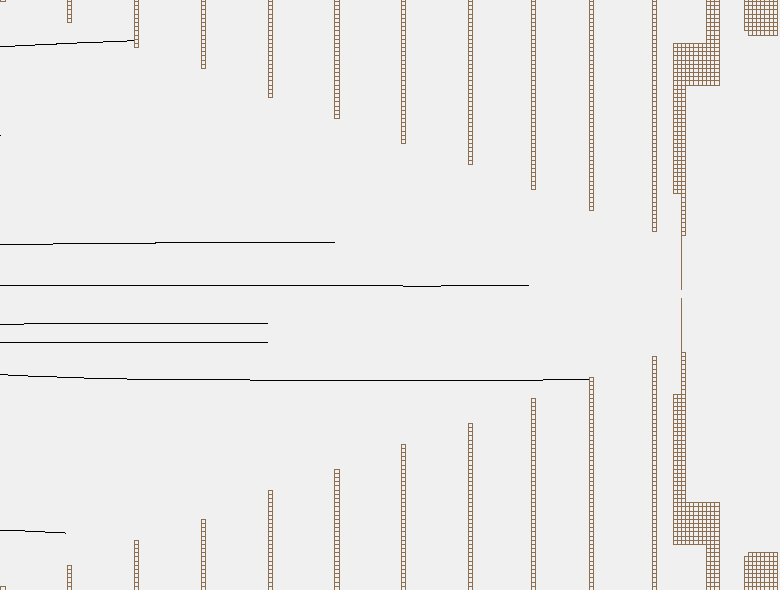
\includegraphics[width=0.35\linewidth]{pics/t01.png}}
\sidesubfloat[]{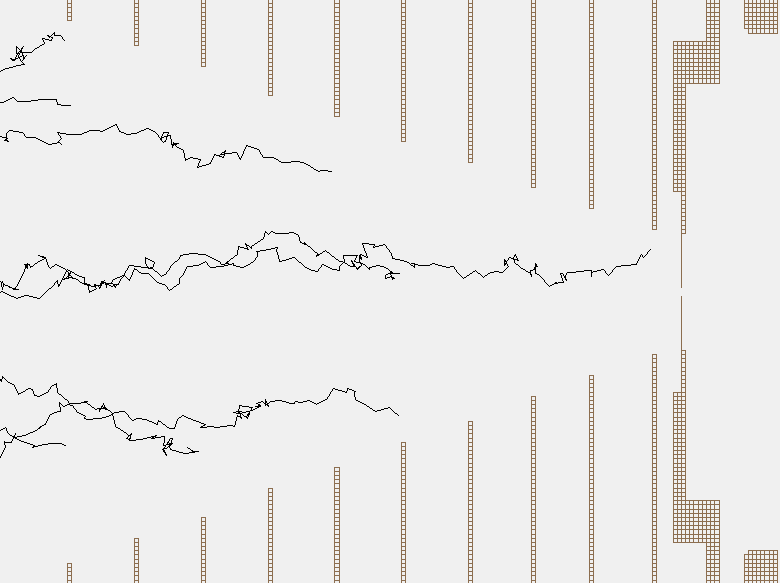
\includegraphics[width=0.35\linewidth]{pics/t11.png}}\\ \bigskip
\sidesubfloat[]{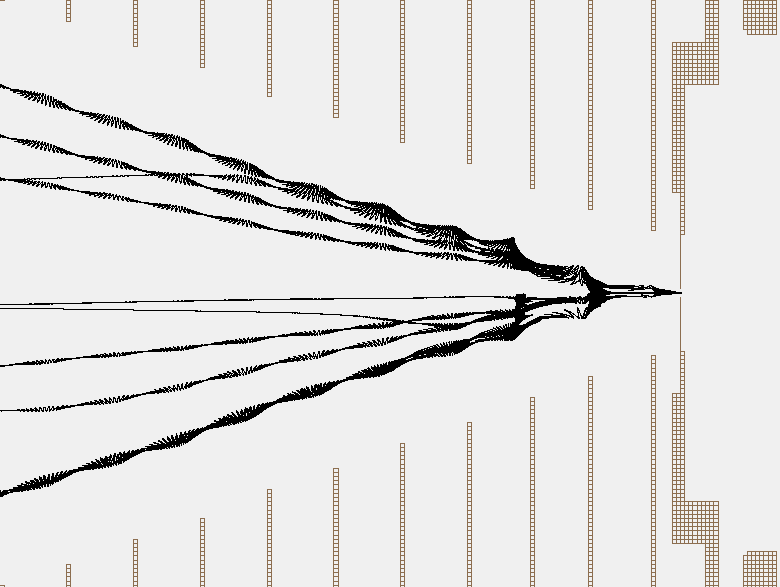
\includegraphics[width=0.35\linewidth]{pics/t02.png}}
\sidesubfloat[]{\includegraphics[width=0.35\linewidth]{pics/t12.png}}\\ \bigskip
\sidesubfloat[]{\includegraphics[width=0.35\linewidth]{pics/t03.png}}
\sidesubfloat[]{\includegraphics[width=0.35\linewidth]{pics/t13.png}}\\ \bigskip
\sidesubfloat[]{\includegraphics[width=0.35\linewidth]{pics/t04.png}}
\sidesubfloat[]{\includegraphics[width=0.35\linewidth]{pics/t14.png}}\\ \bigskip
\end{center}
\caption[Comparison of the trajectories of 10 ions of m/z 19 in different conditions]{Comparison of the trajectories of 10 ions of m/z 19 in different conditions. DC mode (a,b), RF mode: $\Delta \phi$ = 180$^{\circ}$ (c,d), $\Delta \phi$ = 120$^{\circ}$ (e,f) and $\Delta \phi$ = 90$^{\circ}$ (g,h). Note that for the images in the left column there was no diffusion enabled while for the right one the diffusion was enabled.
}\label{fig:traj}
\end{figure}


\subsection{Drift time}
Files:
\begin{itemize}
\item DC mode: \verb|David Olivenza sds model\excel\SDS_drift time_DC|
\item RF mode: \verb|David Olivenza sds model\excel\SDS_drift time_RF|
\end{itemize}

Assuming DC mode (no RF field) and motion in 1D, the forces on the ion:
\begin{equation}
m\frac{d^2x}{dt^2} = eE - k_1\frac{dx}{dt} + k_2 v_{buffer}
\end{equation}
The first term corresponds to the electrostatic force, the second one is the dampening effect due to the collisions with the buffer gas and the third one is the dragging effect due to the non-zero velocity of the buffer gas.
For a steady velocity, i.e. $\frac{d^2x}{dt^2} = 0$, yields
\begin{equation}
\frac{dx}{dt} = \frac{1}{k_1} \left( eE + k_2 v_{buffer} \right)
\end{equation}
So the drift time, i.e. $t_d = L/\frac{dx}{dt}$, is:
\begin{equation}
t_d = \frac{k_1 L}{eE +k_2 v_{buffer}} = \frac{k_1 L}{eV_d/L + k_2 v_{buffer}} = \frac{k_1 L^2/e}{V_d + k_2 L v_{buffer}/e}
\end{equation}
which can be written as:
\begin{equation}
t_d = \frac{C_1}{V_d + C_2}
\label{eq:sds_t}
\end{equation}


Note that:
\begin{equation}
t_d(V_d\rightarrow0) \rightarrow \frac{C_1}{C_2} \approx  t_{buffer}
\end{equation}
This drift time is purely coming from convection. If no electric field was applied to the drift tube, the drift time would be:
\begin{equation}
t_{buffer} = \frac{L}{v_{buffer}} = \frac{9.36\,cm}{100\,m/s} = 936\, \mu s
\end{equation}






\begin{figure}%[h]
\begin{center}
\sidesubfloat[]{\includegraphics[width=0.9\linewidth]{pics/td.eps}}\\
\bigskip
\sidesubfloat[]{\includegraphics[width=0.9\linewidth]{pics/td_RF.eps}}
\end{center}
\caption{SDS model: Plot of the drift time, t$_d$, as a function of drift voltage for (a) DC mode and (b) RF mode. }\label{fig:td_sds}
\end{figure}



\begin{table}[ht]
\centering
\caption{Coefficients of the fits for the drift time shown in figure \ref{fig:td_sds} using equation \ref{eq:sds_t}.}
\label{tb:tdfit}
\begin{tabular}{llccc}
\toprule
\textbf{Mode}&\textbf{Ion} &\textbf{C$_1$ (V $\mu$s)}	&\textbf{C$_2$   (V)} & \textbf{C$_1$/C$_2$ ($\mu$s)}\\ \midrule 
\ldelim\{{4}{20mm}[\parbox{20mm}{DC mode}]&H$_3$O$^+$&2.56$\times$10$^4$	&23.58&	1085.66		\\
&(H$_2$O)H$_3$O$^+$			&4.98$\times$10$^4$	&49.55&	1005.25		\\
&(H$_2$O)$_2$H$_3$O$^+$		&7.43$\times$10$^4$	&75.41&	985.28		\\
&(H$_2$O)$_3$H$_3$O$^+$		&9.66$\times$10$^4$	&96.00&	1005.73		\\
\bottomrule
\ldelim\{{4}{20mm}[\parbox{20mm}{RF mode}]&H$_3$O$^+$&2.33$\times$10$^4$	&14.67&	1589.64		\\
&(H$_2$O)H$_3$O$^+$			&4.80$\times$10$^4$	&43.13&	1112.45		\\
&(H$_2$O)$_2$H$_3$O$^+$		&7.13$\times$10$^4$	&66.17&	1077.07		\\
&(H$_2$O)$_3$H$_3$O$^+$		&9.49$\times$10$^4$	&91.20&	1041.01		\\
\bottomrule
\end{tabular}
\end{table}


\subsection{Buffer gas velocity}
A = 50 cm$^{2}$, flow = 120 sccm = 2 ssc/s (per second) at 1 mbar. mass flow (mdot) = 2000 scc  mbar/s:
\begin{equation}
v \times A \times P = 2000\, scc \, mbar / s
\end{equation}
v = 40 cm/s = 4$\times$10$^{-3}$ mm/$\mu$s = 0.4 m/s

\newpage
\section{Conclusions and further remarks}
From the results here presented it can be inferred that the higher protonation in RF mode at low drift voltage is a consequence of a long drift time (more time to react) together with the higher collisional energy delivered by the RF field.

Also the hydronium signal in RF mode at low drift voltage is of few tens of thousand counts per second (mz19, not 21; mz 21 is tens of counts). However, when the swab is inserted in the TDU and the analyte is desorbed the hydronium signal is not depleted. The simplest explanation for this is that there is enough hydronium to undergo all the proton transfer without being depleted, but it has a low transmission with this conditions in the reaction.


Further steps: implementation of a clustering/declustering process depending upon the collisional energy (after many collisions, change m/z). It could be something like this: at the beginning of the drift tube only clusters are injected and they dissociate with the collisions. 

Also, the newest version of SIMION allows to implement vectorial fields. This can be used to define a more accurate buffer gas velocity and account for turbulent effects after simulating them with computational flow dynamics (CFD) software.
























\chapter{OTHER STUFF}
\markboth{OTHER STUFF}{}




\section{Benzene standard}
Esto lo puedo poner en la descripcion del aparato, a modo de ilustracion




\begin{figure}
  \sidesubfloat[]{\scalebox{0.7}{\begin{tikzpicture}\chemfig{*6(-=-=(-[::-60,,,,white]\phantom{Cl})-=)}\end{tikzpicture}}
  \label{fig:bnz1}}
\qquad \qquad
  \sidesubfloat[]{\scalebox{0.7}{\begin{tikzpicture}\chemfig{
*6(-=(-[::-60]Cl)-=(-[::-60]Cl)-(-[::-60]Cl)=)}\end{tikzpicture}}
\label{fig:bnz2}}
  \caption{Structure of (a) benzene and (b) 1,2,4-trichlorobenzene.}
  \label{fig:bnz}
\end{figure}



\begin{figure}
\scalebox{0.7}{
%\schemedebug{true}
\begin{tikzpicture}
\schemestart
\chemfig[yshift=5em]{*6(-=-=(-[::-60,,,,white]\phantom{Cl})-=)}
\arrow{0}[,0]\+
\chemfig{H_3O^+}
\arrow
\chemfig[yshift=5em]{*6(-=-=(-[::-60]H^+)-=)}
\arrow{0}[,0]  %this arrow is to align
\+
\chemfig{H_2O}
\schemestop
\end{tikzpicture}
}
\label{fig:bnzr}
\caption{Benzene reaction example.}
\end{figure}



\section{DPM - humidity dependence}
\begin{figure}%[h]
\centering
\includegraphics[width=0.48\linewidth]{pics/DPM_clusters_littoral.pdf}
\includegraphics[width=0.48\linewidth]{pics/DPM_BR_lit.pdf}

\includegraphics[width=0.48\linewidth]{pics/DPM_clusters_lynx_humid.pdf}
\includegraphics[width=0.48\linewidth]{pics/DPM_humid_DC_lynx.pdf}

\includegraphics[width=0.48\linewidth]{pics/DPM_clusters_lynx_dry.pdf}
\includegraphics[width=0.48\linewidth]{pics/DPM_dry_DC_lynx.pdf}
\caption{DPM product ion distribution plots from  Littoral (top right) and Lynx in humid (middle right) and in dry (bottom right) conditions in DC mode.}
\label{dpm}
\end{figure}

\begin{figure}%[h]
\centering
\includegraphics[width=0.48\linewidth]{pics/DPM_clusters_humid_RF.pdf}
\includegraphics[width=0.48\linewidth]{pics/DPM_humid_RF.pdf}

\includegraphics[width=0.48\linewidth]{pics/DPM_clusters_dry_RF.pdf}
\includegraphics[width=0.48\linewidth]{pics/DPM_dry_RF.pdf}
\caption{DPM product ion distribution plots from Lynx in humid (top) and  dry (bottom) conditions in RF mode.}
\label{dpm2}
\end{figure}













\chapter{Conclusions and Further Remarks}
\markboth{Conclusions}{}




% from 21.3.19
%David – many thanks for your comments. Yes – I made a mistake in the summary – you are correct. 
%My interpretation of the data is that the BRs are humidity dependent but not the fragmentation pathways – the same ions are seen under dry and humid conditions. But we have already seen that we don’t understand the BRs even under a constant humidity so we cannot expect to understand the effects of changing the humidity – or for that matter changing E/N. 
%Changing the conditions of the hollow cathode – I have no idea – when I last spoke with Chris he suggested it might be worthwhile so you should ask him what he had in mind.
%A different topic. If we have these reactant ions with sufficient energy to fragment ISOF why do we propose more normal energy reactant ions when we study cocaine and the other compounds? My only suggestion is that the highly energetic ions cause massive fragmentation to small ions and are either lost in the noise or ignored or attributed to impurities. Can you have a look at some of the cocaine and analogues spectra and let me know? It’s a problem we have to address before we can publish parallel papers on cocaine and ISOF – and more importantly need to be addressed in your thesis.
%Best wishes - Peter






%\section{Chapter by chapter}
In chapter [] the results [] were presented. 
This concludes....
Further work is needed to elucidate..




























% \blindtext
% \blindtext
% \blindtext




%\nocite{*}
%next line changes bibliography name to references
\renewcommand{\bibname}{References}
\addcontentsline{toc}{chapter}{References}
\printbibliography
\newpage


%now enable appendix numbering format and include any appendices
\appendix

\fancyhead{}    % this cleans the header
\renewcommand{\headrulewidth}{0pt} %this deletes the horizontal line

\begin{appendices}
\chapter{Articles in peer-reviewed journals}\label{chapter:papers}
\markboth{Articles in peer-reviewed journals}{}
            
\section*{Published articles}


The published articles are attached in the following pages.

\begin{refsection}%
%\DeclareFieldFormat{labelnumberwidth}{}%#1}%
\nocite{*}
\printbibliography[keyword=publicado,heading=none] %
%\printbibliography[omitnumbers=true,keyword=publicado,heading=none] %
\end{refsection}%

%\section*{In preparation}

%\section*{Planned}


% tnt
\includepdf[pages=-]{appendix/acs_analchem_6b02982.pdf}
% ketones
\includepdf[pages=-]{appendix/fchem-07-00401.pdf}
% nitroanilines
\includepdf[pages=-]{appendix/nitroanilines.pdf}
% anaesthetics
\includepdf[pages=-]{appendix/ISOF_paper.pdf}
\chapter{Physical properties}


In this appendix some of the physical properties of the substances mentioned in this thesis are shown.






%PA at 300K (kJ/mol). The lowest PA for the molecule is given when more than one protonation site is available.

%Vapor pressure (bar)

%Gas basicity (kJ/mol)












\begin{landscape}
\begin{longtable}[c]{@{}lcccccc@{}}
\toprule
\textbf{Name}        & \textbf{Formula} & \textbf{MW (g/mol)} & \textbf{PA (kJ/mol)} & \textbf{GB (kJ/mol)} &  \textbf{VP (bar)}& \textbf{IE (eV)} \\* \midrule
\endfirsthead
%
\toprule
\textbf{Name}        & \textbf{Formula} & \textbf{MW (g/mol)} & \textbf{PA (kJ/mol)} & \textbf{GB (kJ/mol)} &  \textbf{VP (bar)}& \textbf{IE (eV)} \\* \midrule
\endhead
%
\bottomrule
\endfoot
%
\endlastfoot
%
Cocaine              &                  &                     &                              &                               &                          &                  \\
Benzoylecgonine      &                  &                     &                              &                               &                          &                  \\
Methylecgonine       &                  &                     &                              &                               &                          &                  \\
Ecstasy              &                  &                     &                              &                               &                          &                  \\
Codeine              &                  &                     &                              &                               &                          &                  \\
Morphine             &                  &                     &                              &                               &                          &                  \\
Heroin               &                  &                     &                              &                               &                          &                  \\
2-nitroaniline       &                  &                     &                              &                               &                          &                  \\
3-nitroaniline       &                  &                     &                              &                               &                          &                  \\
4-nitroaniline       &                  &                     &                              &                               &                          &                  \\
Benzoic acid         &                  &                     &                              &                               &                          &                  \\
Methyl benzoate      &                  &                     &                              &                               &                          &                  \\
Ethyl benzoate       &                  &                     &                              &                               &                          &                  \\
Isopropyl benzoate   &                  &                     &                              &                               &                          &                  \\
Benzoic anhydride    &                  &                     &                              &                               &                          &                  \\
Cocaethylene         &                  &                     &                              &                               &                          &                  \\
Methyl echonidine    &                  &                     &                              &                               &                          &                  \\
Diethylene glycol  diethyl ether  &                  &                     &                              &                               &                          &                  \\
Diethylene glycol  dimethyl ether  &                  &                     &                              &                               &                          &                  \\
HMTD                 &                  &                     &                              &                               &                          &                  \\
DPM                  &                  &                     &                              &                               &                          &                  \\
Isoflurane           &                  &                     &                              &                               &                          &                  \\
Sevoflurane          &                  &                     &                              &                               &                          &                  \\
2-Butanone           & C4H8O            & 72.107              & 827.3                        &                               &                          &                  \\
2-Pentanone          & C5H10O           & 86.134              & 832.7                        &                               &                          &                  \\
3-Pentanone          & C5H10O           & 86.134              & 836.8                        &                               & 807                      & 9.31             \\
2-Hexanone           & C6H12O           & 100.161             & -                            &                               &                          &                  \\
3-Hexanone           & C6H12O           & 100.161             & 843.2                        &                               &                          &                  \\
2-Heptanone          & C7H14O           & 114.188             &                              &                               &                          & 9.27             \\
3-Heptanone          & C7H14O           & 114.188             &                              &                               &                          &                  \\
4-Heptanone          & C7H14O           & 114.188             &                              &                               &                          &                  \\
3-Octanone           & C8H16O           & 128.215             &                              &                               &                          &                  \\
2-Nonanone           & C9H18O           & 142.242             &                              &                               &                          &                  \\
3-Nonanone           & C9H18O           & 142.242             &                              &                               &                          &                  \\
2-Decanone           & C10H20O          & 156.269             &                              &                               &                          &                  \\
3-Decanone           & C10H20O          & 156.269             &                              &                               &                          &                  \\
Cyclohexanone        & C6H10O           & 98.145              &                              &                               &                          &                  \\
3-Methyl-2-butanone  & C5H10O           & 86.134              &                              &                               &                          &                  \\
3-Methyl-2-pentanone & C6H12O           & 100.161             &                              &                               &                          &                  \\
2-Methyl-3-pentanone & C6H12O           & 100.161             &                              &                               &                          &                  \\
2-Methyl-3-hexanone  & C7H14O           & 114.188             &                              &                               &                          &                  \\
2-Methyl-3-heptanone & C8H16O           & 128.215             &                              &                               &                          &                  \\* \bottomrule
\end{longtable}
\end{landscape}




%\chapter{Software in Open Access repository}
\markboth{Software}{}
The latest version of the code I have written during my PhD for data analysis and simulations, mainly in Matlab and Lua (for SIMION\textsuperscript{\textregistered}), is available in the Open Source repository Zenodo (\textbf{add link})
\end{appendices}

\end{document}

